\documentclass[11pt]{article}
\usepackage[margin=1.1in]{geometry}
\usepackage{amsmath,amssymb,amsthm,mathtools}
\usepackage{microtype}
\usepackage{xurl}
\usepackage[hidelinks]{hyperref}
\hypersetup{pdftitle={Inflation for Classical Pair-Source Networks: Termination and Quantitative Obstructions},pdfauthor={William Blair}}
\usepackage{booktabs,array}
\usepackage{enumitem}
\usepackage[T1]{fontenc}
\usepackage{lmodern}
\usepackage{graphicx}
\usepackage{tikz}
\usetikzlibrary{arrows.meta,positioning,calc,backgrounds}
\usepackage[font=small,labelfont=bf]{caption}
\captionsetup[figure]{skip=10pt}
\captionsetup[table]{skip=8pt}
\setlength{\textfloatsep}{16pt plus 2pt minus 2pt}
\setlength{\intextsep}{16pt plus 2pt minus 2pt}
\setlength{\floatsep}{14pt plus 2pt minus 2pt}
\usepackage[section]{placeins}
\definecolor{inkblue}{HTML}{245577}
\definecolor{inkrust}{HTML}{A54F2A}
\definecolor{inkgreen}{HTML}{35705B}
\tikzset{observer/.style={circle,draw,fill=white,minimum size=6mm,inner sep=1pt,font=\small},source/.style={rectangle,draw,fill=black!7,minimum size=5mm,inner sep=2pt,font=\small},causal/.style={-{Latex[length=1.6mm]},thin},network/.style={line width=.8pt},every picture/.style={line cap=round}}
\setlength{\emergencystretch}{1.5em}
\setcounter{tocdepth}{1}

\theoremstyle{plain}
\newtheorem{theorem}{Theorem}[section]
\newtheorem{lemma}[theorem]{Lemma}
\newtheorem{proposition}[theorem]{Proposition}
\newtheorem{corollary}[theorem]{Corollary}
\theoremstyle{definition}
\newtheorem{definition}[theorem]{Definition}
\newtheorem{remark}[theorem]{Remark}
\newtheorem{question}[theorem]{Question}

\DeclareMathOperator{\Law}{Law}
\DeclareMathOperator{\Bern}{Bern}
\DeclareMathOperator{\dist}{dist}
\DeclareMathOperator{\TV}{TV}
\newcommand{\Ctri}{\mathcal C_{\triangle}}
\newcommand{\INW}{\mathcal I^{\mathrm{NW}}}
\newcommand{\IAI}{\mathcal I^{\mathrm{AI}}}
\newcommand{\Iexp}{\mathcal I^{\mathrm{exp}}}
\newcommand{\eps}{\varepsilon}
\newcommand{\E}{\mathbb E}
\newcommand{\R}{\mathbb R}
\newcommand{\one}{\mathbf 1}
\newcommand{\tmin}{t_{\min}}

\title{Inflation for Classical Pair-Source Networks:\\ Termination and Quantitative Obstructions}
\newcommand{\repourl}{https://github.com/williamjblair/inflation-termination}
\newcommand{\repo}{\url{\repourl}}

\author{William Blair\\[2pt]\small\texttt{willjblair1@gmail.com}}
\date{September 2026}

\begin{document}
\maketitle
\vspace{-1em}

\begin{abstract}
The classical inflation hierarchy converges to the set of distributions compatible with a correlation scenario, but convergence need not occur at a finite order. We classify finite termination for pair-source scenarios with binary observations: some finite order characterizes compatibility if and only if every connected component of the source graph is a tree of diameter at most three. In that case order two suffices. The classification holds for the Navascués--Wolfe hierarchy and its ancestral-independence and recursively expressible strengthenings; the latter two coincide on pair-source scenarios. The proof reconstructs a model on each double-star and constructs incompatible, strictly positive rational laws accepted at every prescribed order on cycles and the five-observer path. For the triangle and square, the largest total-variation distance of an accepted law from compatibility lies between $c/t$ and $C/\sqrt t$. The upper bound follows from a convex-order argument and depends only on the number of observed outcomes. A separate triangle construction gives a first rejecting order of $\Theta(d^{-1/3})$ along an explicit family at distance $d$ from compatibility, and yields a worst required order of $2^{\Theta(B)}$ for rational inputs of $B$ bits. Exact certificates accompany the finite computations. The classification for binary observations and finite latent alphabets, together with several triangle results, is formalized in Lean.
\end{abstract}

\begingroup
\footnotesize
\makeatletter
\renewcommand\l@section{\@dottedtocline{1}{0em}{1.8em}}
\makeatother
\tableofcontents
\endgroup
\clearpage

\section{Introduction}\label{sec:intro}

A correlation scenario has independent latent sources and observed variables that respond to the sources reaching them. Its compatible laws form a nonconvex set. Finite latent-cardinality bounds make this set semialgebraic, but an explicit characterization is unavailable even for the classical triangle with binary observations \cite{Fritz2012,RGW2018}. Inflation tests compatibility by copying each source $t$ times and asking for a joint law on the copied observations with prescribed marginals \cite{WSF2019}. Navascués and Wolfe proved asymptotic completeness of their hierarchy and asked whether, for a fixed scenario and fixed observed alphabets, some finite order already decides compatibility \cite{NW2020}. They identified the triangle as a possible counterexample.

We answer this question for pair-source scenarios, in which each source is shared by exactly two observers. Such a scenario is a finite simple graph $G$: observers are vertices and sources are edges. We then study the order needed to reject incompatible laws near the compatible set.

\subsection{Main results}

\paragraph{Termination classification.}
For binary observations, a pair-source scenario has a finite characterizing order if and only if every connected component is a tree of diameter at most three, or \emph{double-star}. In that case order two suffices. Otherwise, for every prescribed order there is an incompatible, strictly positive rational law accepted at that order (Theorem~\ref{thm:classification}). This classification holds for the Navascués--Wolfe (NW), ancestral-independence (AI) and recursively expressible tests. The last two coincide on pair-source scenarios.

The proof reconstructs a model on each double-star. Every other connected graph contains an induced cycle or a five-vertex path; explicit witnesses on these subgraphs extend to the ambient graph. Figure~\ref{fig:classification} shows the dividing line.

\begin{figure}[!htbp]
\centering
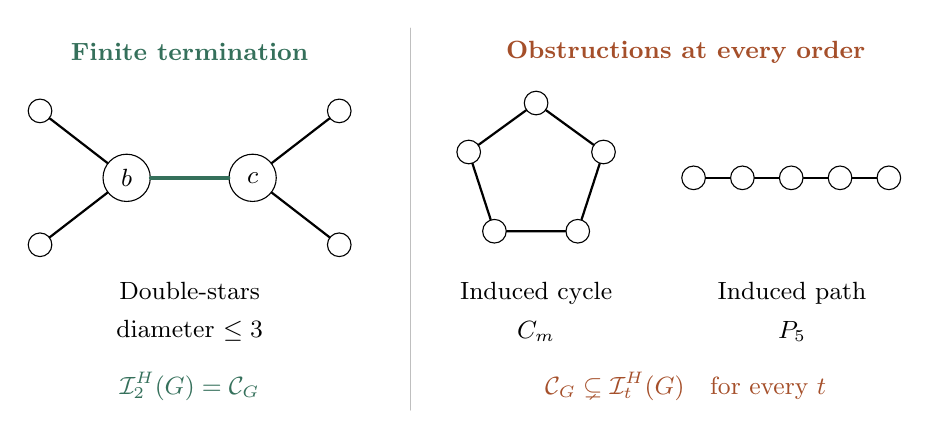
\begin{tikzpicture}[x=1cm,y=1cm]
\node[font=\small\bfseries,inkgreen] at (1.9,1.6) {Finite termination};
\node[observer] (b) at (1.1,0) {$b$}; \node[observer] (c) at (2.7,0) {$c$};
\draw[network,inkgreen,line width=1.4pt] (b)--(c);
\foreach \i/\x/\y in {1/0/0.85,2/0/-0.85,3/3.8/0.85,4/3.8/-0.85}{\node[observer,minimum size=3mm] (l\i) at (\x,\y) {};}
\draw[network] (l1)--(b)--(l2) (l3)--(c)--(l4);
\node[font=\small,align=center] at (1.9,-1.7) {Double-stars\\[3pt]diameter $\le3$};
\node[font=\small,inkgreen] at (1.9,-2.65) {$\mathcal I_2^H(G)=\mathcal C_G$};
\draw[black!25] (4.7,1.9)--(4.7,-2.95);
\node[font=\small\bfseries,inkrust] at (8.2,1.6) {Obstructions at every order};
\foreach \i/\a in {0/90,1/18,2/-54,3/-126,4/162}{\node[observer,minimum size=3mm] (v\i) at ($(6.3,0.05)+(\a:.9)$) {};}
\draw[network] (v0)--(v1)--(v2)--(v3)--(v4)--(v0);
\node[font=\small,align=center] at (6.3,-1.7) {Induced cycle\\[3pt]$C_m$};
\foreach \i in {0,...,4}{\node[observer,minimum size=3mm] (p\i) at (8.3+0.62*\i,0) {};}
\draw[network] (p0)--(p1)--(p2)--(p3)--(p4);
\node[font=\small,align=center] at (9.55,-1.7) {Induced path\\[3pt]$P_5$};
\node[font=\small,inkrust] at (8.2,-2.65) {$\mathcal C_G\subsetneq\mathcal I_t^H(G)\quad\text{for every }t$};
\end{tikzpicture}
\caption{The classification for binary pair-source scenarios. Vertices denote observers and edges independent pair sources. A graph terminates precisely when each component is a double-star. Every other component contains an induced cycle or $P_5$, from which an incompatible order-$t$ law extends to the whole graph. Here $H$ is NW, AI or exp.}\label{fig:classification}
\end{figure}


\paragraph{Quantitative convergence.}
Let $H_t^H(G)$ be the largest total-variation distance from compatibility among laws accepted at order $t$ by hierarchy $H$. For the triangle and square we prove
\[
\frac{c_G}{t}\le H_t^H(G)\le\frac{C_G}{\sqrt t},
\]
with explicit positive constants (Corollary~\ref{cor:brackets}). The lower bounds use parity laws and corrected Fourier densities. The upper bound follows from a convex-order comparison and applies to any correlation scenario with $K$ joint outcomes, with $C_G=\sqrt{K-1}/2$ (Theorem~\ref{thm:convexorder}). On the square, increasing the NW order by a factor at most $3/2$ enforces all AI prescriptions (Theorem~\ref{thm:orderconversion}). Finite certificates also separate these tests at specified orders.

\paragraph{Rejecting orders near the boundary.}
A second triangle construction places independent defects in a cube of copy indices. It gives passing witnesses for
\[
Q(\eps,r)=\eps\,\delta_{000}+(1-\eps)\Bern(r)^{\otimes3},
\qquad r\le(1-\eps)^{t-1},
\]
where $\Bern(r)(1)=r$. For $P_\eps=Q(\eps,1-\tfrac12\eps^{2/3})$, a fan inequality gives a matching rejecting-order exponent:
\[
\tmin^H(P_\eps)=\Theta(\eps^{-1/3})
=\Theta\bigl(d_{\TV}(P_\eps,\Ctri)^{-1/3}\bigr).
\]
We compute the leading distance constant and bound the rejecting-order constants (Proposition~\ref{prop:family}, Theorem~\ref{thm:distance}). This exponent describes this family; the worst-case bounds above concern all accepted laws. For rational binary-triangle inputs of at most $B$ bits, the largest first rejecting order is $2^{\Theta(B)}$ (Proposition~\ref{prop:bits}). A promised distance $\delta>0$ gives the bound $\lfloor(K-1)/(4\delta^2)\rfloor+1$ for any fixed correlation scenario.

\subsection{Relation to prior work}\label{sec:prior}

\paragraph{Finite termination.}
Navascués and Wolfe prove order-two termination for stars and exhibit triangle-incompatible laws that pass order two \cite[Section 4.1]{NW2020}. Our reconstruction extends their source-disjointness argument to double-stars, including their four-on-line example; the cycle and five-path witnesses complete the classification. Henson, Lal and Pusey~\cite{HensonLalPusey2014} ask which causal structures are characterized by observed conditional independences. Their criterion differs already on the four-on-line scenario, which fails that criterion but terminates at order two. The strict gap between expressible and AI prescriptions exhibited by Wolfe, Spekkens and Fritz~\cite{WSF2019} uses an observed node with observed children. Lemma~\ref{lem:rootsink} rules out that gap for the root-sink graphs considered here. The finite nonattainment example for polynomial optimization in~\cite{NW2020} concerns a scenario in which every law is compatible; our obstruction is to finite compatibility testing itself.

\paragraph{Inequalities and witnesses.}
The defect construction violates Finner's inequality \cite{Finner1992,Renou2019}. The five-path obstruction uses the bilocal square-root inequality of Branciard, Rosset, Gisin and Pironio~\cite{BranciardRossetGisinPironio2012}, with the endpoint observers serving as settings. Cycle incompatibility uses parity rigidity, developed for the triangle by Boreiri et al.\ \cite{BoreiriEtAl2023,BoreiriEtAl2025}; Renou and Beigi~\cite{RenouBeigi2022PRA} prove token-counting rigidity on rings. We give the needed classical parity proofs for arbitrary latent spaces and stochastic responses. Our symmetric triangle parity family is among the families studied by da Silva, Pozas-Kerstjens and Parisio~\cite{daSilvaPozasKerstjensParisio2025}. Inflation has also certified nonlocality along continuous families \cite{PozasKerstjensGisinRenou2023}; here the quantitative question is how the rejecting order grows as an incompatible law approaches the classical set.

The fan inequality follows the marginal-polytope method of~\cite[Section IV.D]{WSF2019}, also used for the wagon-wheel and web inequalities of Fraser and Wolfe~\cite{FraserWolfe2018}. We derive a formula indexed by the order and a second-moment bound. The witness densities and count-moment reductions use Fourier characters and Krawtchouk polynomials, standard tools in coding theory~\cite{MacWilliamsSloane1977}.

\paragraph{Convergence and effectivity.}
The convex-order estimate removes the source-count factor from the finite-sampling bound of~\cite{NW2020}. Related convergence results for postselected inflation~\cite{Gitton2022} and the combinatorial hierarchy~\cite{Fraser2020} also depend on source parameters. The sampling comparison is related to Hoeffding's convex-order inequality~\cite[Theorem 4]{Hoeffding1963}. The input-size upper bound combines our distance estimate with finite latent cardinality~\cite{RGW2018}, real quantifier elimination~\cite{BasuPollackRoy2006} and a polynomial root bound. Quantum inflation and its convergent variants~\cite{WolfeEtAl2021QuantumInflation,LigthartGachechiladzeGross2023} concern different compatible sets; their finite-termination questions remain outside the classification here.\par


\paragraph{Organization.}
Section~\ref{sec:setup} defines the scenarios and tests, with the triangle as an example. Section~\ref{sec:classification} proves the classification. Sections~\ref{sec:cyclequant} and~\ref{sec:main} give the convergence bounds and the defect-family analysis; Section~\ref{sec:input} derives the distance and input-size consequences. Open problems and verification scope follow in Sections~\ref{sec:open} and~\ref{sec:repro}. The appendices contain the root-sink proof, order-conversion and threshold details, certificate formats and supplementary inequalities.

\section{Pair-source scenarios and inflation}\label{sec:pairsource}\label{sec:setup}

\providecommand{\Cscen}[1]{\mathcal C_{#1}}
\providecommand{\supp}{\operatorname{supp}}

\subsection{Scenarios}

\begin{definition}[Pair-source scenario]\label{def:pairsource}
Let $G=(V,E)$ be a finite simple graph without isolated vertices. The associated scenario has one latent source $S_e$ for each edge $e\in E$, taking values in an arbitrary measurable space, and one observed variable $O_v$ with a finite alphabet $\mathcal O_v$ for each vertex $v\in V$. The sources are mutually independent, and
\[
O_v\sim\kappa_v\bigl(\cdot\mid(S_e)_{e\ni v}\bigr),
\]
conditionally independently across $v$ given the sources. Write $\Cscen{G}$ for the set of joint laws of $(O_v)_{v\in V}$ obtained in this way. Unless stated otherwise every $\mathcal O_v$ is $\{0,1\}$, and we call these the binary observations.
\end{definition}

Each source is read by exactly the two endpoints of its edge. We write $C_m$ for the cycle on $m$ vertices, $P_n$ for the path on $n$ vertices, and $\Ctri=\Cscen{C_3}$.

Sources shared by three or more observers, and latent variables with latent parents, are outside this definition; see Remark~\ref{rem:hypergraph}.

Assign each vertex $v$ an independent random seed and append it to the source of one edge at $v$, to be ignored by the other endpoint. The graph is unchanged and the seed makes the response at $v$ deterministic, so stochastic and deterministic responses generate the same set $\Cscen{G}$ \cite{WSF2019}. The assumption that no vertex is isolated ensures an incident edge is available.

\subsection{Inflation at order \texorpdfstring{$t$}{t}}

\begin{definition}[Order-$t$ inflation]\label{def:ginflation}
Fix $t\ge1$ and write $E(v)=\{e\in E:v\in e\}$ for the edges at $v$ and $E(W)=\bigcup_{v\in W}E(v)$ for a vertex set $W$. The order-$t$ inflation of $G$ has independent copies $S_e^1,\dots,S_e^t$ of each source, and for every vertex $v$ and every index tuple $i\in[t]^{E(v)}$ one copied observation
\[
O_v^{\,i}\sim\kappa_v\bigl(\cdot\mid(S_e^{\,i_e})_{e\in E(v)}\bigr),
\]
all conditionally independent given the source copies. Writing $r$ also for the constant tuple with value $r$, the \emph{row} $r\in[t]$ is the family $(O_v^{\,r})_{v\in V}$, and the $t$ rows form the diagonal.
\end{definition}

A vertex of degree $d$ has $t^d$ copies, so the inflation carries $\sum_v t^{\deg v}$ observed variables. The group $\prod_{e\in E}S_t$ acts on the copy labels: $\sigma=(\sigma_e)_{e\in E}$ sends the label $i$ to $\sigma(i)$ with $\sigma(i)_e=\sigma_e(i_e)$, and hence sends $O_v^{\,i}$ to $O_v^{\,\sigma(i)}$. Each $\sigma$ maps rows to rows when all its components are equal, and otherwise mixes them.

Call a probability law on $\prod_{v\in V}\bigl(\mathcal O_v\bigr)^{[t]^{E(v)}}$ a \emph{table} of order $t$. Each of the three tests asks for a table with prescribed marginals.

\begin{definition}[Navascués--Wolfe feasible set]\label{def:gNW}\label{def:NW}
$P\in\INW_t(G)$ if there is a table $\Gamma_t$ of order $t$ such that
\begin{enumerate}[label=(\roman*),nosep]
\item $\Gamma_t$ is invariant under $\prod_{e\in E}S_t$; and
\item its diagonal law is a tensor power,
\[
\Law_{\Gamma_t}\bigl((O_v^{\,r})_{v\in V}\ :\ r=1,\dots,t\bigr)=P^{\otimes t}.
\]
\end{enumerate}
\end{definition}

\begin{definition}[Injectable sets and the AI feasible set]\label{def:gAI}\label{def:AI}
A set $S$ of copied observations is \emph{injectable} if the map $\pi$ that erases copy indices is injective on $S$ and any two members of $S$ whose vertices share an edge carry the same index on that edge \cite[Definition~4]{WSF2019}. Equivalently, $S$ is injectable if and only if there are a vertex set $W\subseteq V$ and an assignment $\iota:E(W)\to[t]$ with
\[
S=\bigl\{O_v^{\,\iota|_{E(v)}}\ :\ v\in W\bigr\},
\]
in which case $\pi(S)=W$. Two sets of copied observations are \emph{ancestrally independent} if the sets of source copies they read are disjoint. $P\in\IAI_t(G)$ if $P\in\INW_t(G)$ with a witness $\Gamma_t$ under which every injectable set $S$ has marginal $P_{\pi(S)}$ and every union of pairwise ancestrally independent injectable sets has the product of the corresponding marginals.
\end{definition}

For the equivalence in Definition~\ref{def:gAI}, given $S$ injectable, let $W=\pi(S)$ and let $\iota(e)$ be the common index carried on $e$ by the members of $S$ at the endpoints of $e$ that lie in $W$, which is well defined by the agreement requirement; conversely every set of the displayed form is injectable. For the triangle this reproduces the description in Appendix~\ref{app:injectable}: the injectable sets are the subsets of the copied triangles.

\begin{definition}[Recursively expressible feasible set]\label{def:gexp}\label{def:exp}
Expressible sets of copied observations are generated from injectable sets by the two rules of \cite[Definition~7]{WSF2019}, read in the inflated causal graph of Definition~\ref{def:ginflation}: if $X$ and $Y$ are $d$-separated by $Z$ and the laws on $X\cup Z$ and on $Y\cup Z$ are prescribed, then
\[
p(x,y,z)=\frac{p(x,z)\,p(y,z)}{p(z)}\quad\text{where }p(z)>0,\qquad p(x,y,z)=0\quad\text{where }p(z)=0,
\]
is prescribed on $X\cup Y\cup Z$; and every marginal of a prescribed set is prescribed. $P\in\Iexp_t(G)$ if $P\in\IAI_t(G)$ with a witness satisfying every prescription so generated.
\end{definition}

\begin{proposition}[Soundness]\label{prop:gsound}
For every pair-source scenario $G$ and every $t\ge1$,
\begin{equation}\label{eq:nested}
\Cscen{G}\subseteq\Iexp_t(G)\subseteq\IAI_t(G)\subseteq\INW_t(G).
\end{equation}
\end{proposition}

\begin{proof}
The two inclusions on the right hold because each test adds prescriptions to the previous one. For the first, realize $P$ by a model, run the model on the inflated source family of Definition~\ref{def:ginflation}, and let $\Gamma_t$ be the law of the copied observations. Permuting the copies of one source permutes independent identically distributed variables, so $\Gamma_t$ is invariant. Distinct rows read disjoint source copies and each row has law $P$, so the diagonal law is $P^{\otimes t}$. An injectable set $S$ reads, for each $v\in\pi(S)$, the copies indexed by a single global assignment $\iota$, so the joint law of $S$ is that of $(O_v)_{v\in\pi(S)}$ in the original model, namely $P_{\pi(S)}$. Ancestrally independent sets read disjoint source copies, hence are independent. The inflated model is a causal model for the inflated graph, so all conditional independences read off that graph hold, and the expressible prescriptions follow by induction on their generation.
\end{proof}


For fixed $P$, each prescription fixes a marginal of the table, so all three tests are linear feasibility problems. Restricting a table to fewer copy indices preserves the conditions; thus the feasible sets decrease with $t$. The Navascués--Wolfe hierarchy is asymptotically complete, $\INW_t(G)\downarrow\Cscen{G}$ \cite{NW2020}. Consequently, for an incompatible law and $H\in\{\mathrm{NW},\mathrm{AI},\mathrm{exp}\}$, the first rejecting order
\[
\tmin^H(P)=\min\{t\ge1:P\notin\mathcal I_t^H(G)\}
\]
is finite. We use total variation $d_{\TV}(P,Q)=\tfrac12\sum_x|P(x)-Q(x)|$ and the distances
\[
d_{\TV}(P,\mathcal C)=\inf_{Q\in\mathcal C}d_{\TV}(P,Q),\qquad
d_2(P,\mathcal C)=\inf_{Q\in\mathcal C}\|P-Q\|_2.
\]
The finite latent-cardinality theorem of Rosset, Gisin and Wolfe~\cite{RGW2018} makes $\Cscen{G}$ compact and semialgebraic for fixed finite observed alphabets.

\subsection{The triangle as a worked example}\label{sec:triangle}

The triangle has independent sources $X,Y,Z$ and observations
\[
A\sim\kappa_A(\cdot\mid X,Z),\qquad
B\sim\kappa_B(\cdot\mid X,Y),\qquad
C\sim\kappa_C(\cdot\mid Z,Y).
\]
Its order-$t$ inflation carries $3t^2$ observations, indexed as
\[
A^{ij}=A(X_i,Z_j),\qquad B^{ik}=B(X_i,Y_k),\qquad C^{jk}=C(Z_j,Y_k),\qquad i,j,k\in[t].
\]
This notation allows stochastic responses as in Definition~\ref{def:ginflation}. A copied triangle is $\Delta_{ijk}=\{A^{ij},B^{ik},C^{jk}\}$, with source copies $X_i,Z_j,Y_k$; the diagonal triangles are $\Delta_{\ell\ell\ell}$ for $\ell\in[t]$.

\begin{figure}[!htbp]
\centering
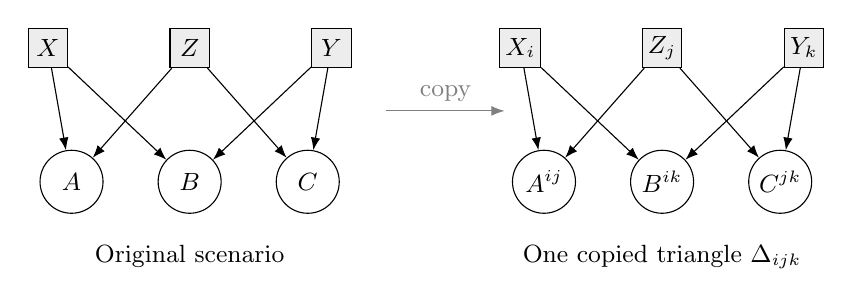
\begin{tikzpicture}[x=1cm,y=1cm]
\foreach \off/\suffix in {0/a,6/b}{
\node[source] (X\suffix) at (\off,1.2) {\ifnum\off=0 $X$\else $X_i$\fi};
\node[source] (Z\suffix) at (\off+1.8,1.2) {\ifnum\off=0 $Z$\else $Z_j$\fi};
\node[source] (Y\suffix) at (\off+3.6,1.2) {\ifnum\off=0 $Y$\else $Y_k$\fi};
\node[observer,minimum size=8mm] (A\suffix) at (\off+0.3,-.5) {\ifnum\off=0 $A$\else $A^{ij}$\fi};
\node[observer,minimum size=8mm] (B\suffix) at (\off+1.8,-.5) {\ifnum\off=0 $B$\else $B^{ik}$\fi};
\node[observer,minimum size=8mm] (C\suffix) at (\off+3.3,-.5) {\ifnum\off=0 $C$\else $C^{jk}$\fi};
\draw[causal] (X\suffix)--(A\suffix); \draw[causal] (X\suffix)--(B\suffix);
\draw[causal] (Z\suffix)--(A\suffix); \draw[causal] (Z\suffix)--(C\suffix);
\draw[causal] (Y\suffix)--(B\suffix); \draw[causal] (Y\suffix)--(C\suffix);
}
\node[font=\small] at (1.8,-1.45) {Original scenario};
\node[font=\small] at (7.8,-1.45) {One copied triangle $\Delta_{ijk}$};
\draw[-{Latex},black!50] (4.3,.4)--node[above,font=\small] {copy}(5.8,.4);
\end{tikzpicture}
\caption{Sources (squares) and observations (circles) in the triangle. Each copied observation carries the indices of its two source parents. Diagonal triangles $\Delta_{\ell\ell\ell}$ use disjoint source copies; the NW test requires their joint law to be $P^{\otimes t}$. The full order-$t$ table includes all $3t^2$ copied observations.}\label{fig:triangle}
\end{figure}


We omit the graph argument from $\INW_t$, $\IAI_t$ and $\Iexp_t$ when discussing the triangle. Definition~\ref{def:NW} is the full-table symmetric formulation of \cite[equations (16)--(19)]{NW2020}; its lower-degree diagonal conditions follow by marginalization. Their cyclic indexing and ours describe the same copied variables. The injectable sets are precisely the subsets of copied triangles (Appendix~\ref{app:injectable}). The AI conditions additionally prescribe products for sets with disjoint copied ancestors, for example
\[
\Law(A^{12},B^{21},C^{12})=P_A\otimes P_B\otimes P_C.
\]
The NW test does not impose this relation at order two.

For later use, every compatible triangle law satisfies the event form of Finner's inequality,
\begin{equation}\label{eq:finner}
P(000)^2\le P_A(0)P_B(0)P_C(0).
\end{equation}
Lemma~\ref{lem:finner} proves it for arbitrary latent spaces and stochastic responses \cite{Finner1992,Renou2019}.


\section{The termination classification}\label{sec:classification}

\providecommand{\Cscen}[1]{\mathcal C_{#1}}


\begin{definition}[Double-star]\label{def:doublestar}
A \emph{double-star} is a graph with a distinguished edge $\{b,c\}$, the \emph{central edge}, such that every other vertex is adjacent to exactly one of $b$ and $c$ and to nothing else. Equivalently, a double-star is a tree of diameter at most three. Single edges and stars are double-stars.
\end{definition}

\begin{theorem}[Termination classification]\label{thm:classification}\label{thm:classification-intro}
Let $G$ be a finite simple graph without isolated vertices, with binary observations. The following are equivalent.
\begin{enumerate}[label=(\alph*),nosep]
\item $\INW_t(G)=\Cscen{G}$ for some finite $t$.
\item $\IAI_t(G)=\Cscen{G}$ for some finite $t$.
\item $\Iexp_t(G)=\Cscen{G}$ for some finite $t$.
\item Every connected component of $G$ is a double-star.
\end{enumerate}
When they hold,
\[
\INW_2(G)=\IAI_2(G)=\Iexp_2(G)=\Cscen{G}.
\]
When they fail, for every $t\ge1$ there is a strictly positive rational law
\[
P\in\Iexp_t(G)\setminus\Cscen{G}\subseteq\IAI_t(G)\setminus\Cscen{G}\subseteq\INW_t(G)\setminus\Cscen{G}.
\]
\end{theorem}

The graph and the alphabets stay fixed as $t$ grows; only the law $P$ varies. The proof combines Theorem~\ref{thm:doublestar} with Theorems~\ref{thm:cycle} and \ref{thm:fivepath} through the exhaustion lemma below.

\subsection{Structural lemmas}

In the inflated graph every source copy is a root and every copied observation is a sink. This structure makes the AI and expressible prescriptions coincide; Appendix~\ref{app:rootsink} proves the equivalence.

\begin{definition}[Shared-parent graph and AI sets]\label{def:sharedparent}
For a set $W$ of copied observations, the \emph{shared-parent graph} on $W$ joins two members when they read a common source copy. Call $W$ an \emph{AI set} if it is a union of pairwise ancestrally independent injectable sets.
\end{definition}

\begin{lemma}[Root-sink lemma]\label{lem:rootsink}
Let $G$ be a pair-source scenario and $t\ge1$.
\begin{enumerate}[label=(\roman*),nosep]
\item A set $W$ of copied observations is an AI set if and only if every connected component of its shared-parent graph is injectable.
\item A table satisfies every expressible prescription of Definition~\ref{def:gexp} if and only if it satisfies the injectable and ancestral-independence prescriptions of Definition~\ref{def:gAI}.
\end{enumerate}
In particular $\Iexp_t(G)=\IAI_t(G)$ for every $t$.
\end{lemma}


Lemma~\ref{lem:rootsink} identifies the two stronger tests but says nothing about the Navascués--Wolfe test, and imposes no causal model on the table as a whole.

\paragraph{Source-disjoint blocks.}

\begin{lemma}[Source-disjoint independence]\label{lem:sourcedisjoint}
Let $t\ge2$ and $P\in\INW_t(G)$. If $U,W\subseteq V$ satisfy $E(U)\cap E(W)=\varnothing$, then
\[
P_{U\cup W}=P_U\otimes P_W.
\]
\end{lemma}

\begin{proof}
Let $\Gamma$ be a witness. Let $\sigma$ be the element of $\prod_eS_t$ that transposes the copy indices $1$ and $2$ on every edge of $E(W)$ and fixes all other indices. For $u\in U$ every edge at $u$ lies outside $E(W)$, so $\sigma$ fixes $O_u^{\,1}$; for $w\in W$ every edge at $w$ lies in $E(W)$, so $\sigma$ sends $O_w^{\,1}$ to $O_w^{\,2}$. Invariance of $\Gamma$ gives
\[
\Law\bigl((O_u^{\,1})_{u\in U},(O_w^{\,1})_{w\in W}\bigr)=\Law\bigl((O_u^{\,1})_{u\in U},(O_w^{\,2})_{w\in W}\bigr).
\]
The left side is the marginal of row $1$, namely $P_{U\cup W}$. The right side reads $U$-coordinates from row $1$ and $W$-coordinates from row $2$, and the two rows are independent with law $P$ each, so it is $P_U\otimes P_W$.
\end{proof}

Two vertices joined by an edge have that edge in both incidence sets, so the hypothesis says exactly that $U$ and $W$ are disjoint and no edge joins them. Iterating the lemma with $U$ a single block and $W$ the union of the others gives mutual independence of any family of pairwise source-disjoint blocks. In particular the observed law of a disconnected graph factors over its components from order two on.

\paragraph{Induced subgraphs.}

\begin{lemma}[Induced-subgraph transport]\label{lem:transport}
Let $H$ be an induced subgraph of $G$ in which no vertex is isolated, and let $\mathcal J\in\{\INW,\IAI,\Iexp\}$.
\begin{enumerate}[label=(\roman*),nosep]
\item If $Q\in\Cscen{G}$ then $Q_{V(H)}\in\Cscen{H}$.
\item If $P_H\in\mathcal J_t(H)$ then $P:=P_H\otimes\Bern(1/2)^{\otimes(V\setminus V(H))}\in\mathcal J_t(G)$.
\item $d_{\TV}(P,\Cscen{G})\ge d_{\TV}(P_H,\Cscen{H})$. In particular, if $P_H\notin\Cscen{H}$ then $P\notin\Cscen{G}$.
\end{enumerate}
\end{lemma}

For restriction, sources crossing the subgraph boundary can be absorbed into incident retained sources. For extension, the copied observations in $H$ ignore all boundary indices, and the remaining observations are independent fair bits. Marginalization then gives the distance bound. Appendix~\ref{app:transport} gives the full proof.

Part (ii) preserves strict positivity and rationality of the target, since the appended factor is the fair-bit law.

\subsection{Reduction to cycles and paths}

\begin{lemma}[Exhaustion]\label{lem:exhaustion}
Let $K$ be a finite connected graph that has at least one edge and is not a double-star. Then $K$ has an induced subgraph isomorphic to a cycle $C_m$ with $m\ge3$ or to the path $P_5$.
\end{lemma}

\begin{proof}
Suppose first that $K$ contains a cycle, and let $C$ be one of minimum length. A chord of $C$ would split it into two shorter cycles, so $C$ has no chords and is induced. Its length is at least $3$.

Suppose next that $K$ is a tree. We claim that a tree of diameter at most three is a double-star. If the diameter is $1$ then $K$ is a single edge. If it is $2$ then $K$ is a star. Let the diameter be $3$ and fix a geodesic $u_0u_1u_2u_3$. Let $w$ be a vertex other than $u_1$ and $u_2$, and consider the unique path from $w$ to $u_1$. If it avoids $u_2$, then it also avoids $u_3$, since the path from $u_3$ to $u_1$ passes through $u_2$; so concatenating with $u_1u_2u_3$ gives a path and $d(w,u_3)=d(w,u_1)+2\le3$, whence $d(w,u_1)=1$. If it contains $u_2$, then the path from $w$ to $u_2$ avoids $u_1$ and hence $u_0$, and the same argument with $u_0$ gives $d(w,u_2)=1$. Every vertex is therefore adjacent to $u_1$ or $u_2$, and $K$ is a double-star with central edge $u_1u_2$.

So a tree that is not a double-star has diameter at least $4$. Take a geodesic of length at least $4$ and let $v_0,\dots,v_4$ be five consecutive vertices on it. Any edge of $K$ among them other than the four geodesic edges would create a cycle in a tree, so the induced subgraph on $\{v_0,\dots,v_4\}$ is $P_5$.
\end{proof}

\begin{proof}[Proof of Theorem~\ref{thm:classification}]
Assume (d). Each component is a double-star with binary observations, so Theorem~\ref{thm:doublestar} and Corollary~\ref{cor:disjointunions} give $\INW_2(G)=\Cscen{G}$. With Proposition~\ref{prop:gsound},
\[
\Cscen{G}\subseteq\Iexp_2(G)\subseteq\IAI_2(G)\subseteq\INW_2(G)=\Cscen{G},
\]
so all four sets coincide and (a), (b), (c) hold at $t=2$.

Assume (d) fails, and fix $t\ge1$. Some component $K$ of $G$ is not a double-star, and $K$ has an edge because $G$ has no isolated vertices. By Lemma~\ref{lem:exhaustion}, $K$ has an induced subgraph $H$ isomorphic to $C_m$ for some $m\ge3$ or to $P_5$; since $K$ is induced in $G$, so is $H$, and $H$ has no isolated vertices. Theorem~\ref{thm:cycle} in the first case and Theorem~\ref{thm:fivepath} in the second supply a strictly positive rational law
\[
P_H\in\Iexp_t(H)\setminus\Cscen{H}.
\]
Let $P=P_H\otimes\Bern(1/2)^{\otimes(V\setminus V(H))}$. By Lemma~\ref{lem:transport}(ii), $P\in\Iexp_t(G)$, and by Lemma~\ref{lem:transport}(iii), $P\notin\Cscen{G}$. It is strictly positive and rational because $P_H$ is. By Proposition~\ref{prop:gsound} the same law lies in $\IAI_t(G)$ and in $\INW_t(G)$, so none of the three tests equals $\Cscen{G}$ at order $t$. As $t$ was arbitrary, (a), (b) and (c) all fail.

This proves the equivalence and both quantitative assertions.
\end{proof}

For $m=3$ the witness of Theorem~\ref{thm:cycle} is a second nonterminating family for the triangle, alongside the defect construction of Theorem~\ref{thm:main}.

\begin{remark}[Larger observed alphabets]\label{rem:alphabets}
Fix finite alphabets $\mathcal O_v$ with $|\mathcal O_v|\ge2$. The classification is unchanged, with a different order in the terminating case. If some component is not a double-star, regard the binary law $P$ of Theorem~\ref{thm:classification} as a law on $\prod_v\mathcal O_v$ supported on $\{0,1\}^V$. A compatible realization of such a law has responses that leave $\{0,1\}$ with probability zero, hence is a binary realization, so the law remains incompatible; and its witness, read in the larger alphabets, satisfies the same prescriptions. The transferred law is supported on the binary sub-alphabet, so the strict positivity in Theorem~\ref{thm:classification} is a statement about binary observations. If every component is a double-star, Theorem~\ref{thm:doublestar} gives termination at
\[
T=\max\bigl(\{2\}\cup\{|\mathcal O_v|:v\text{ a leaf}\}\bigr),
\]
the leaves being taken with respect to a choice of central edge in each component; the bound does not involve the alphabets at the central vertices.
\end{remark}

\begin{remark}[Scenarios that are not pair-source]\label{rem:hypergraph}
Let three observers read one common source. That source can carry a sample of the whole observed triple, so every law on the three outcomes is compatible and the order-one test already characterizes the compatible set, while the observed adjacency graph of this scenario is the triangle, which does not terminate at any order. The adjacency graph alone therefore carries no classification once source hyperedges are allowed.
\end{remark}

\subsection{Finite reconstruction on double-stars}\label{sec:doublestar}

\providecommand{\Cscen}[1]{\mathcal C_{#1}}
\providecommand{\supp}{\operatorname{supp}}

Fix a double-star $G$ in the sense of Definition~\ref{def:doublestar}: two central vertices $b,c$ joined by the central edge $y=\{b,c\}$, left leaves $\ell_1,\dots,\ell_p$ joined to $b$ by edges $e_1,\dots,e_p$, and right leaves $r_1,\dots,r_q$ joined to $c$ by edges $f_1,\dots,f_q$. Observed alphabets $\mathcal O_v$ are finite and arbitrary. Put
\[
T=\max\bigl(\{2\}\cup\{|\mathcal O_{\ell_s}|\}_{s\le p}\cup\{|\mathcal O_{r_j}|\}_{j\le q}\bigr).
\]

In the order-$T$ inflation the leaves have one index each, and the centres have one index per incident edge. Write
\[
L_s^{\,m}=O_{\ell_s}^{\,m},\qquad R_j^{\,m}=O_{r_j}^{\,m},\qquad
B^{\,\mathbf i,n}=O_b^{\,(\mathbf i,n)},\qquad C^{\,n,\mathbf k}=O_c^{\,(n,\mathbf k)},
\]
where $m,n\in[T]$, $\mathbf i\in[T]^p$ records the index on each $e_s$, and $\mathbf k\in[T]^q$ the index on each $f_j$. Row $m$ consists of $L_s^{\,m}$, $R_j^{\,m}$, $B^{\,m,m}$ and $C^{\,m,m}$, with $\mathbf i$ and $\mathbf k$ constant equal to $m$.

For a law $P$ on $\prod_v\mathcal O_v$ write $P(\beta,\gamma,\xi,\zeta)$ for the probability that $O_b=\beta$, $O_c=\gamma$, $O_{\ell_s}=\xi_s$ for all $s$ and $O_{r_j}=\zeta_j$ for all $j$.

\begin{theorem}[Double-star reconstruction]\label{thm:doublestar}
For every double-star $G$ with finite observed alphabets,
\[
\INW_T(G)=\Cscen{G}.
\]
\end{theorem}

\begin{proof}
The inclusion $\Cscen{G}\subseteq\INW_T(G)$ is Proposition~\ref{prop:gsound}. Let $P\in\INW_T(G)$ and let $\Gamma$ be a witness at order $T$. We recover a model for $P$ in four steps.

\medskip
\emph{(i) The leaves and all their copies are independent.}
Distinct leaves have disjoint incidence sets, each consisting of a single edge, so Lemma~\ref{lem:sourcedisjoint}, available because $T\ge2$, applies to one leaf against the union of the others and, iterated, gives
\begin{equation}\label{eq:leafprod}
P_{\mathrm{leaf}}(\xi,\zeta):=P\bigl(O_{\ell_s}=\xi_s\ \forall s,\ O_{r_j}=\zeta_j\ \forall j\bigr)=\prod_{s}P_{\ell_s}(\xi_s)\prod_{j}P_{r_j}(\zeta_j).
\end{equation}
Under $\Gamma$ the $T$ rows are independent with law $P$ each, and the leaf entries of a single row are independent by \eqref{eq:leafprod}. Every copied leaf observation occurs in exactly one row, so the whole family $\{L_s^{\,m},R_j^{\,m}\}$ is independent under $\Gamma$, with $L_s^{\,m}\sim P_{\ell_s}$ and $R_j^{\,m}\sim P_{r_j}$.

\medskip
\emph{(ii) A positive conditioning event.}
For each left leaf choose $x_s^{\,1},\dots,x_s^{\,T}\in\mathcal O_{\ell_s}$ so that every symbol of $\supp P_{\ell_s}$ occurs in the list, which is possible because $T\ge|\mathcal O_{\ell_s}|$; fill the remaining positions with repetitions of a supported symbol. Choose $z_j^{\,1},\dots,z_j^{\,T}$ for each right leaf in the same way. Let
\[
E=\bigl\{L_s^{\,m}=x_s^{\,m}\ \forall s,m\bigr\}\cap\bigl\{R_j^{\,m}=z_j^{\,m}\ \forall j,m\bigr\}.
\]
By (i),
\begin{equation}\label{eq:QE}
\Gamma(E)=\prod_{s,m}P_{\ell_s}(x_s^{\,m})\prod_{j,m}P_{r_j}(z_j^{\,m})>0.
\end{equation}

\medskip
\emph{(iii) The conditional marginal of the two centres.}
Fix $\mathbf i\in[T]^p$ and $\mathbf k\in[T]^q$. Choose permutations $\sigma_s\in S_T$ of the copy indices of $e_s$ with $\sigma_s(1)=i_s$, permutations $\tau_j\in S_T$ of those of $f_j$ with $\tau_j(1)=k_j$, and the identity on the central edge $y$. The resulting element of the symmetry group carries row $m$ to
\[
\Bigl(B^{\,(\sigma_s(m))_s,\,m},\ C^{\,m,(\tau_j(m))_j},\ \bigl(L_s^{\,\sigma_s(m)}\bigr)_s,\ \bigl(R_j^{\,\tau_j(m)}\bigr)_j\Bigr),
\]
which for $m=1$ is $\bigl(B^{\,\mathbf i,1},C^{\,1,\mathbf k},(L_s^{\,i_s})_s,(R_j^{\,k_j})_j\bigr)$. By invariance the joint law of these $T$ images equals the joint law of the $T$ rows, namely $P^{\otimes T}$. As $m$ runs over $[T]$ the index $\sigma_s(m)$ runs over $[T]$, so every copied leaf observation occurs exactly once among the images and the event $E$ is determined by them. Marginalizing the images of rows $2,\dots,T$ over their two centre entries and using \eqref{eq:leafprod},
\[
\Gamma\bigl(B^{\,\mathbf i,1}=\beta,\ C^{\,1,\mathbf k}=\gamma,\ E\bigr)
=P\bigl(\beta,\gamma,x^{\mathbf i},z^{\mathbf k}\bigr)
\prod_s\prod_{m\ne i_s}P_{\ell_s}(x_s^{\,m})\prod_j\prod_{m\ne k_j}P_{r_j}(z_j^{\,m}),
\]
where $x^{\mathbf i}=(x_s^{\,i_s})_s$ and $z^{\mathbf k}=(z_j^{\,k_j})_j$. Dividing by \eqref{eq:QE} and using \eqref{eq:leafprod} once more,
\begin{equation}\label{eq:condmarg}
\Gamma\bigl(B^{\,\mathbf i,1}=\beta,\ C^{\,1,\mathbf k}=\gamma\mid E\bigr)
=P\bigl(O_b=\beta,\ O_c=\gamma\ \bigm|\ O_{\ell_s}=x_s^{\,i_s}\ \forall s,\ O_{r_j}=z_j^{\,k_j}\ \forall j\bigr),
\end{equation}
the conditioning event on the right having positive probability whenever every $x_s^{\,i_s}$ and $z_j^{\,k_j}$ is supported. This identity is the finite-order step, a statement about the witness derived from symmetry and the diagonal law alone.

\medskip
\emph{(iv) Two response tables and fresh sources.}
For $\xi\in\prod_s\supp P_{\ell_s}$ pick positions $\mathbf i(\xi)$ with $x_s^{\,i_s(\xi)}=\xi_s$, and for $\zeta\in\prod_j\supp P_{r_j}$ pick $\mathbf k(\zeta)$ with $z_j^{\,k_j(\zeta)}=\zeta_j$. Under the conditional law $\Gamma(\cdot\mid E)$ define the random maps
\[
F(\xi)=B^{\,\mathbf i(\xi),1},\qquad G(\zeta)=C^{\,1,\mathbf k(\zeta)},
\]
with arbitrary fixed values on unsupported arguments. Both are functions of the same table, so the pair $(F,G)$ has a joint law $\mu$, and \eqref{eq:condmarg} reads
\begin{equation}\label{eq:mutable}
\mu\bigl(F(\xi)=\beta,\ G(\zeta)=\gamma\bigr)=P\bigl(O_b=\beta,O_c=\gamma\mid\xi,\zeta\bigr)
\end{equation}
for all supported $\xi,\zeta$.

Now take fresh independent sources: let the central source be $Y^*=(F,G)\sim\mu$, let the source of $e_s$ be $X_s^*\sim P_{\ell_s}$ and the source of $f_j$ be $Z_j^*\sim P_{r_j}$, all mutually independent. Respond by
\[
O_{\ell_s}=X_s^*,\qquad O_{r_j}=Z_j^*,\qquad O_b=F(X_1^*,\dots,X_p^*),\qquad O_c=G(Z_1^*,\dots,Z_q^*).
\]
Each response reads only the sources of its incident edges: $b$ reads $X_1^*,\dots,X_p^*$ and $Y^*$, and $c$ reads $Y^*$ and $Z_1^*,\dots,Z_q^*$. This is a model for the scenario $G$, and by \eqref{eq:mutable} and \eqref{eq:leafprod} its observed law is
\[
\prod_sP_{\ell_s}(\xi_s)\prod_jP_{r_j}(\zeta_j)\,\mu\bigl(F(\xi)=\beta,G(\zeta)=\gamma\bigr)
=P_{\mathrm{leaf}}(\xi,\zeta)\,P(\beta,\gamma\mid\xi,\zeta)=P(\beta,\gamma,\xi,\zeta).
\]
Unsupported leaf values are never sampled, so the arbitrary choices there do not matter. Hence $P\in\Cscen{G}$.
\end{proof}

The conditional law supplies the distribution of the central response tables. The model then samples this central source independently of fresh leaf sources, as required by the graph. A central source with
\(
|\mathcal O_b|^{\prod_s|\supp P_{\ell_s}|}\,|\mathcal O_c|^{\prod_j|\supp P_{r_j}|}
\)
values suffices: a left response table is a map on the product of the left leaf supports, and likewise on the right. Empty products equal one.

\begin{corollary}[Binary observations]\label{cor:doublestarbinary}
For a double-star with binary observations, $\INW_2(G)=\Cscen{G}$.
\end{corollary}

\begin{proof}
All leaf alphabets have two elements, so $T=2$.
\end{proof}

\begin{corollary}[Four-observer path]\label{cor:path}
Consider $A(X)$, $B(X,Y)$, $C(Y,Z)$, $D(Z)$, the path $P_4$ with $A$ and $D$ at the ends. Then $\INW_T(P_4)=\Cscen{P_4}$ with $T=\max\{2,|\mathcal O_A|,|\mathcal O_D|\}$. For binary endpoints $T=2$, whatever the finite alphabets of $B$ and $C$.
\end{corollary}

\begin{proof}
$P_4$ is the double-star with central edge $\{B,C\}$, one left leaf $A$ and one right leaf $D$; apply Theorem~\ref{thm:doublestar}, whose bound involves only the leaf alphabets.
\end{proof}
This is the four-on-line scenario of \cite[Figure~8]{NW2020}. Navascu\'es and Wolfe list it with the triangle among the scenarios whose compatible set is cut out by inequality constraints, show that order two does not suffice for the triangle, and leave the four-on-line case open. The corollary settles it at order two for binary endpoints.

\begin{corollary}[Disjoint unions]\label{cor:disjointunions}
Let $G$ be a disjoint union of double-stars $G_1,\dots,G_n$ with orders $T_1,\dots,T_n$ as above, and let $T=\max\{2,T_1,\dots,T_n\}$. Then $\INW_T(G)=\Cscen{G}$.
\end{corollary}

\begin{proof}
Let $P\in\INW_T(G)$ with witness $\Gamma$. Distinct components are source-disjoint, so Lemma~\ref{lem:sourcedisjoint}, iterated, gives $P=\bigotimes_aP_{V(G_a)}$. The restriction of $\Gamma$ to the copied observations at the vertices of $G_a$ is a table for the order-$T$ inflation of $G_a$: it is invariant under permutations of the copy indices of the edges of $G_a$, and its diagonal law is the corresponding marginal of $P^{\otimes T}$, namely $\bigl(P_{V(G_a)}\bigr)^{\otimes T}$. Hence $P_{V(G_a)}\in\INW_T(G_a)\subseteq\INW_{T_a}(G_a)$, the inclusion because discarding the copy indices outside $[T_a]$ leaves a witness at order $T_a$. Theorem~\ref{thm:doublestar} now gives $P_{V(G_a)}\in\Cscen{G_a}$. Realize each component by its own model on its own independent source family; the joint observed law is the product, which is $P$.
\end{proof}

A star is the case $q=0$, with $c$ one of its leaves. There the bound of Theorem~\ref{thm:doublestar} is not sharp: order two suffices with arbitrary finite alphabets \cite[Section 4.1]{NW2020}, by taking independent sources equal to the leaf values and letting the centre respond with its conditional law given them. Theorem~\ref{thm:doublestar} adds the central edge, where the two centres share a source and the leaf values on the two sides must be assembled into one pair of response tables.

\providecommand{\Cscen}[1]{\mathcal C_{#1}}
\providecommand{\Csq}{\mathcal C_{\square}}
\providecommand{\Ccyc}{\mathcal C_{C_m}}
\providecommand{\Real}{\operatorname{Re}}
\providecommand{\sgn}{\operatorname{sgn}}

\subsection{Cycles}\label{sec:cycles}

Section~\ref{sec:pairsource} writes the three finite tests for an arbitrary pair-source scenario. For every cycle and every order we construct a strictly positive law that the strongest of them accepts and that no model produces, with a quantitative separation from compatibility. Section~\ref{sec:cyclequant} refines the distance bound for the triangle and square.

Throughout, the $m$-cycle $C_m$, $m\ge3$, has observed variables $O_0,\dots,O_{m-1}$ and sources $S_0,\dots,S_{m-1}$, indices read modulo $m$, with $O_v$ a child of $S_{v-1}$ and $S_v$; the copied observations of Definition~\ref{def:ginflation} are written $O_v^{ij}$, children of $S_{v-1,i}$ and $S_{v,j}$. The triangle is $C_3$, with $\Ctri=\Cscen{C_3}$, read as $A=O_0$, $B=O_1$, $C=O_2$ and $X=S_0$, $Y=S_1$, $Z=S_2$; the square is $C_4$, written $\square$, read as $A(X,W)$, $B(X,Y)$, $C(Y,Z)$, $D(Z,W)$ with $X=S_0$, $Y=S_1$, $Z=S_2$, $W=S_3$.

\subsubsection{Parity witnesses on every cycle}\label{sec:cycleparity}

\begin{lemma}[Auxiliary parity density]\label{lem:parityaux}
For $N\ge1$ and $q\ge0$ let
\begin{equation}\label{eq:Hdensity}
H_{N,q}(s)=2^{-N}\sum_{\substack{S\subseteq[N]\\|S|\text{ even}}}(-q)^{|S|/2}\prod_{w\in S}s_w,
\qquad s\in\{-1,1\}^N .
\end{equation}
Then $H_{N,q}$ is normalized, its characters are
\begin{equation}\label{eq:Hmoments}
\E_{H_{N,q}}\Bigl[\prod_{w\in S}s_w\Bigr]=
\begin{cases}
0,&|S|\text{ odd},\\
(-q)^{|S|/2},&|S|\text{ even},
\end{cases}
\end{equation}
and if $N^2q\le1/4$ then $H_{N,q}(s)\ge\tfrac23\,2^{-N}>0$ for every $s$.
\end{lemma}

\begin{proof}
Normalization and \eqref{eq:Hmoments} are orthogonality of the characters of $\{-1,1\}^N$ under the uniform measure. For positivity, $\binom N{2j}\le N^{2j}$, so
\[
\bigl|2^NH_{N,q}(s)-1\bigr|\le\sum_{j\ge1}\binom N{2j}q^j\le\sum_{j\ge1}(N^2q)^j\le\sum_{j\ge1}4^{-j}=\tfrac13 . \qedhere
\]
\end{proof}

For $F\subseteq\{0,\dots,m-1\}$ let $\partial F=\{w:|F\cap\{w,w+1\}|=1\}$ be the set of edges of $C_m$ incident to an odd number of vertices of $F$. Every vertex meets two edges, so $|\partial F|$ is even.

\begin{definition}[Cycle parity family]\label{def:cycletarget}
For $m\ge3$ and $q\ge0$ let $P_{m,q}$ be the signed measure on $\{-1,1\}^m$ with density $2^{-m}\sum_F(-q)^{|\partial F|/2}\prod_{v\in F}o_v$ against the counting measure, so that it has total mass $1$ and
\begin{equation}\label{eq:cycletarget}
\E_{P_{m,q}}\Bigl[\prod_{v\in F}O_v\Bigr]=(-q)^{|\partial F|/2}\qquad\text{for every }F .
\end{equation}
\end{definition}

If $m^2q\le1/4$ then $P_{m,q}$ is a probability law, being the law of $(\sigma_{v-1}\sigma_v)_{v=0}^{m-1}$ for $\sigma\sim H_{m,q}$. The exact ranges in the two cases we use are wider.

Taking $F$ the whole vertex set gives $\E[\prod_vO_v]=1$, so wherever $P_{m,q}$ is a probability law the product of all $m$ signs is $1$ almost surely; taking $F$ a contiguous arc gives mean $-q$. For $m=3$ the family is the parity-even law with observed means $x,y,z$,
\begin{equation}\label{eq:paritylaw}
\Pi(x,y,z)(\alpha,\beta,\gamma)=\tfrac14\bigl(1+x\alpha+y\beta+z\gamma\bigr)\ \text{ on }\alpha\beta\gamma=1,\qquad P_{3,q}=\Pi(-q,-q,-q),
\end{equation}
which is a probability law exactly for $0\le q\le1/3$; and for $m=4$ it is the square parity family $P_q:=P_{4,q}$ with atoms
\begin{equation}\label{eq:squaretarget}
\tfrac18(1-6q+q^2)\ \text{ at }0000,\qquad
\tfrac18(1-q^2)\ \text{ at }0011,0110,1001,1100,\qquad
\tfrac18(1+q)^2\ \text{ at }0101,1010,1111,
\end{equation}
zero on odd parity, in the convention $0\leftrightarrow+1$. It is a law exactly for $0\le q\le3-2\sqrt2$.

Fix $t\ge1$, put $N=mt$ and draw auxiliary signs $s=(s_{v,i})_{v\in\{0,\dots,m-1\},\,i\in[t]}$ from $H_{N,q}$. Define every copied observation by
\begin{equation}\label{eq:cyclewitness}
O_v^{ij}=s_{v-1,i}\,s_{v,j}.
\end{equation}
For a set $F$ of copied observations let $\partial F$ denote the set of copied sources occurring an odd number of times in $\prod_{O\in F}O$; each copied observation contributes two incidences, so $|\partial F|$ is even, and \eqref{eq:Hmoments} gives
\begin{equation}\label{eq:masterchar}
\E\Bigl[\prod_{O\in F}O\Bigr]=(-q)^{|\partial F|/2}.
\end{equation}

\begin{lemma}[Boundaries of prescribed characters]\label{lem:boundary}
Let $F_1,\dots,F_r$ be pairwise ancestrally independent injectable sets of copied observations of $C_m$ and let $U_i\subseteq F_i$. Then each $\partial U_i$ has even cardinality and contains at most one copy of each source, so it is empty or meets at least two source families; the sets $\partial U_1,\dots,\partial U_r$ are pairwise disjoint; and $\partial(U_1\cup\dots\cup U_r)=\bigsqcup_i\partial U_i$, which again is empty or meets at least two source families. Moreover $\partial U_i$ is the image, under erasure of copy indices, of the boundary of the corresponding original observed set.
\end{lemma}

\begin{proof}
An injectable set contains at most one copied observation over each original vertex and its ancestry contains at most one copy of each original source, so $\partial U_i$ contains at most one coordinate from each family; being of even cardinality it is empty or has at least two elements in distinct families. Erasing copy indices carries the incidence count of $U_i$ to that of its image, which gives the last claim. Ancestrally independent sets have disjoint ancestries, hence disjoint coordinate sets and disjoint boundaries, and the boundary of a union of sets with disjoint ancestries is the disjoint union of the boundaries. If that union is nonempty then some $\partial U_i$ is nonempty and already meets two families.
\end{proof}

\begin{lemma}[The parity witness passes every prescription]\label{lem:cyclewitness}
Let $m\ge3$, $t\ge1$ and $0<q\le1/(4m^2t^2)$. The auxiliary density is strictly positive, and the law of \eqref{eq:cyclewitness} is a witness placing $P_{m,q}$ in $\IAI_t(C_m)=\Iexp_t(C_m)$.
\end{lemma}

\begin{proof}
Positivity of $H_{N,q}$ holds since $N^2q=m^2t^2q\le1/4$. The density \eqref{eq:Hdensity} is symmetric in the $N$ coordinates, so the witness is invariant under independent permutations of the copy indices of each source. By Lemma~\ref{lem:boundary} an injectable set $F$ has $\partial F$ equal to the boundary of its image, so \eqref{eq:masterchar} and \eqref{eq:cycletarget} give it the prescribed marginal of $P_{m,q}$. For pairwise ancestrally independent injectable $F_1,\dots,F_r$ and any $U_i\subseteq F_i$, Lemma~\ref{lem:boundary} and \eqref{eq:masterchar} give
\[
\E\Bigl[\prod_i\prod_{O\in U_i}O\Bigr]=(-q)^{\frac12\sum_i|\partial U_i|}=\prod_i\E\Bigl[\prod_{O\in U_i}O\Bigr],
\]
and characters determine a law on a finite sign cube, so the blocks are independent with the prescribed marginals. The diagonal rows are pairwise ancestrally independent injectable copied cycles, so the diagonal law is $P_{m,q}^{\otimes t}$. Lemma~\ref{lem:rootsink} supplies the recursive prescriptions.
\end{proof}

The witness is a law on the copied observations, not the output of an inflated model: under $H_{N,q}$ the auxiliary signs are correlated across families.

\begin{lemma}[Exact parity rigidity]\label{lem:parityrigidity}
Let $R\in\Ctri$ with $ABC=1$ almost surely. Then there are $\sigma,\tau,\upsilon\in[-1,1]$ with $(\E A,\E B,\E C)=(\sigma\tau,\sigma\upsilon,\tau\upsilon)$. In particular $\E A\cdot\E B\cdot\E C\ge0$.
\end{lemma}

\begin{proof}
Absorb the response seeds into incident sources, so that $A=A(X,Z)$, $B=B(X,Y)$, $C=C(Z,Y)$ are deterministic signs. For $\mu_Y$-almost every $y$ the identity $A(X,Z)B(X,y)C(Z,y)=1$ holds for $\mu_X\otimes\mu_Z$-almost every $(X,Z)$; fix such a $y_0$ and put $S(X)=B(X,y_0)$, $T(Z)=C(Z,y_0)$, so that $A=ST$ almost surely. Substituting in $ABC=1$ gives $\bigl(S(X)B(X,Y)\bigr)\bigl(T(Z)C(Z,Y)\bigr)=1$ almost surely. Write $B'=SB$ and $C'=TC$. Conditionally on $Y$ these are independent signs, and they agree almost surely, so each equals a function $U(Y)$ almost surely. Hence $A=ST$, $B=SU$, $C=TU$ almost surely, and independence of the three sources gives the means with $\sigma=\E S$, $\tau=\E T$, $\upsilon=\E U$. Their product is $(\sigma\tau\upsilon)^2$.
\end{proof}

Rigidity of the parity-perfect (parity token-counting) triangle correlations is prior work: the exact statement is due to Boreiri, Girardin, Ulu, Lipka-Bartosik, Brunner and Sekatski \cite{BoreiriEtAl2023}, and Boreiri, Ulu, Brunner and Sekatski \cite{BoreiriEtAl2025} give a noise-robust form (a compatible law with parity error $\epsilon$ is within $3\epsilon$ of a parity-perfect compatible law); Lemma~\ref{lem:quantrigidity} is a moment form of that robustness. Renou and Beigi \cite{RenouBeigi2022PRA,RenouBeigi2022PRL} prove rigidity of token-counting distributions on every ring scenario with bipartite sources; their statements concern integer token counts rather than parity, so they do not contain the lemma below, but they are the prior rigidity results on cycles. We give the two proofs because we need the statements for arbitrary latent alphabets and stochastic responses, and because the constant of Lemma~\ref{lem:quantrigidity} enters the distance bounds below.

\begin{lemma}[Quantitative parity rigidity]\label{lem:quantrigidity}
Let $R\in\Ctri$ and $W=\E_R[ABC]$. Then
\[
\max\{\E_RA,\ \E_RB,\ \E_RC\}\ \ge\ -4(1-W).
\]
\end{lemma}

\begin{proof}
Let $a(x,z)$, $b(x,y)$, $c(z,y)$ be the conditional means of $A$, $B$, $C$ given the sources; they take values in $[-1,1]$, and since the three responses use independent private randomness, $W=\E[abc]$ and $\E_RA=\E[a]$, with the expectations over the independent sources $X,Y,Z$. We use two inequalities: for $p,r\in[-1,1]$,
\begin{equation}\label{eq:pr}
|p-r|\le1-pr,
\end{equation}
since for $p\ge r$ the difference $(1-pr)-(p-r)=(1-p)(1+r)$ is nonnegative, and for $u,w\in[-1,1]$,
\begin{equation}\label{eq:uw}
|u+w|\ge2uw,
\end{equation}
since for $uw\le0$ the right side is nonpositive and for $u,w$ of the same sign $|u|+|w|-2|u||w|=|u|(1-|w|)+|w|(1-|u|)\ge0$.

Choose $y_0$ with $\E_{X,Z}[1-a(X,Z)b(X,y_0)c(Z,y_0)]\le1-W$; it exists because the average over $Y$ of the left side is $1-W$. Put $S(X)=b(X,y_0)$ and $T(Z)=c(Z,y_0)$. By \eqref{eq:pr} with $p=a$, $r=ST$,
\[
\E|a-ST|\le\E[1-aST]\le1-W,\qquad\text{so}\qquad |\E[a]-\E[S]\,\E[T]|\le1-W,
\]
using the independence of $X$ and $Z$. Next let $u(y)=\E_X[S(X)b(X,y)]$ and $w(y)=\E_Z[T(Z)c(Z,y)]$, both in $[-1,1]$, and $\upsilon(y)=\sgn(u(y)+w(y))$. By \eqref{eq:uw},
\begin{multline*}
\E_Y[1-\upsilon u]+\E_Y[1-\upsilon w]=\E_Y[2-|u+w|]\le2-2\E_Y[uw]\\
=2-2\E[STbc]\le2-2\bigl(W-\E|a-ST|\bigr)\le4(1-W),
\end{multline*}
where $\E_Y[uw]=\E[S(X)T(Z)b(X,Y)c(Z,Y)]$ by independence of the sources and $\E[STbc]\ge\E[abc]-\E|ST-a|$ because $|bc|\le1$. Hence $\E_Y[1-\upsilon u]\le4(1-W)$ and $\E_Y[1-\upsilon w]\le4(1-W)$. By \eqref{eq:pr} with $p=b(X,Y)$ and $r=S(X)\upsilon(Y)$,
\[
\E|b-S\upsilon|\le\E[1-bS\upsilon]=\E_Y[1-\upsilon u]\le4(1-W),\qquad\text{so}\qquad|\E[b]-\E[S]\,\E[\upsilon]|\le4(1-W),
\]
and likewise $|\E[c]-\E[T]\,\E[\upsilon]|\le4(1-W)$. Write $\sigma=\E[S]$, $\tau=\E[T]$, $\nu=\E[\upsilon]$. If all three means were below $-4(1-W)$, then $\sigma\tau\le\E[a]+(1-W)<0$, $\sigma\nu<0$ and $\tau\nu<0$, whose product $(\sigma\tau\nu)^2$ is nonnegative, a contradiction.
\end{proof}
For $W=1$ the lemma recovers the consequence of Lemma~\ref{lem:parityrigidity} that at least one mean is nonnegative. A compatible law at total-variation distance $\delta$ from a parity-perfect law has $1-W\le2\delta$, so the lemma also replaces the repair step of \cite{BoreiriEtAl2025}: we construct no repaired model, and the bound holds for arbitrary latent alphabets and stochastic responses.

\begin{lemma}[Distance of the cycle family]\label{lem:cycledistance}
Let $m\ge3$ and let $q>0$ be such that $P_{m,q}$ is a probability law. Then $d_{\TV}(P_{m,q},\Ccyc)\ge q/10$; in particular $P_{m,q}\notin\Ccyc$.
\end{lemma}

\begin{proof}
As illustrated in Figure~\ref{fig:cycle-reduction}, partition $\{0,\dots,m-1\}$ into three nonempty contiguous arcs $\Lambda_1,\Lambda_2,\Lambda_3$ and let $\varphi(o)=(V_1,V_2,V_3)$ with $V_r=\prod_{v\in\Lambda_r}o_v$. If $R\in\Ccyc$, then $\varphi_*R\in\Ctri$: the three sources on the arc boundaries are independent, each arc product is a function of the two boundary sources adjacent to its arc together with the sources internal to that arc, and those internal sources can be absorbed as private randomness of the arc. Each $\partial\Lambda_r$ has two elements, and $\partial(\Lambda_1\cup\Lambda_2)=\partial\Lambda_3$, so \eqref{eq:cycletarget} gives
\[
\varphi_*P_{m,q}=\Pi(-q,-q,-q).
\]

Let $R\in\Ccyc$ and $\delta=d_{\TV}(P_{m,q},R)$. Total variation does not increase under $\varphi$, so $Q=\varphi_*R\in\Ctri$ satisfies $d_{\TV}(\Pi(-q,-q,-q),Q)\le\delta$. Since $|\E_Pf-\E_Qf|\le2d_{\TV}(P,Q)$ for $|f|\le1$, the parity $W=\E_Q[V_1V_2V_3]$ satisfies $1-W\le2\delta$ and each mean $\E_QV_r$ is at most $-q+2\delta$. Lemma~\ref{lem:quantrigidity} gives $-q+2\delta\ge-4(1-W)\ge-8\delta$, that is $\delta\ge q/10$.
\end{proof}

\begin{figure}[!htbp]
\centering
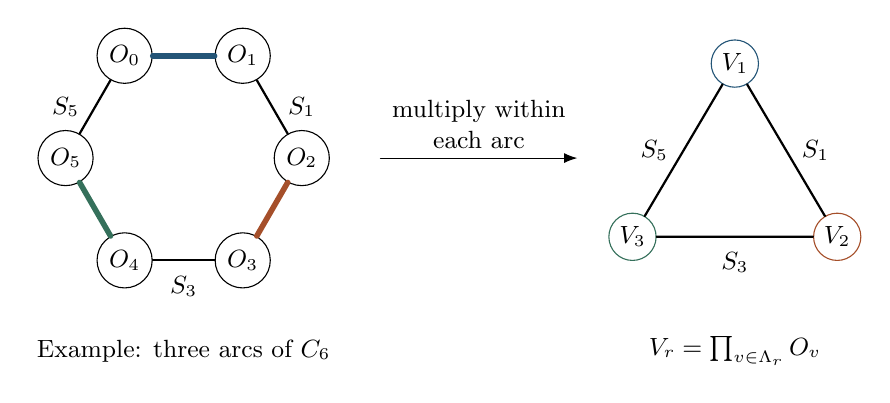
\begin{tikzpicture}[x=1cm,y=1cm]
\foreach \i/\a in {0/120,1/60,2/0,3/-60,4/-120,5/180}{\node[observer,minimum size=7mm] (o\i) at (\a:1.5) {$O_\i$};}
\draw[network,inkblue,line width=2pt] (o0)--(o1);
\draw[network,inkrust,line width=2pt] (o2)--(o3);
\draw[network,inkgreen,line width=2pt] (o4)--(o5);
\draw[network] (o1)--node[right=2pt,font=\small] {$S_1$}(o2);
\draw[network] (o3)--node[below=2pt,font=\small] {$S_3$}(o4);
\draw[network] (o5)--node[left=2pt,font=\small] {$S_5$}(o0);
\draw[-{Latex}] (2.5,0)--node[above,align=center,font=\small] {multiply within\\each arc}(5,0);
\node[observer,draw=inkblue] (v1) at (7,1.2) {$V_1$};
\node[observer,draw=inkrust] (v2) at (8.3,-1) {$V_2$};
\node[observer,draw=inkgreen] (v3) at (5.7,-1) {$V_3$};
\draw[network] (v1)--node[right=2pt,font=\small] {$S_1$}(v2)--node[below=2pt,font=\small] {$S_3$}(v3)--node[left=2pt,font=\small] {$S_5$}(v1);
\node[font=\small] at (0,-2.45) {Example: three arcs of $C_6$};
\node[font=\small] at (7,-2.45) {$V_r=\prod_{v\in\Lambda_r}O_v$};
\end{tikzpicture}
\caption{Reducing cycle incompatibility to triangle parity rigidity. Partition any cycle into three nonempty contiguous arcs and multiply the observations within each arc. The three boundary sources form a triangle; internal sources become private randomness. The target reduces to $\Pi(-q,-q,-q)$, and total variation cannot increase under this map.}\label{fig:cycle-reduction}
\end{figure}


\begin{theorem}[Cycles at every order]\label{thm:cycle}
Let $m\ge3$ and $t\ge1$, put
\[
q=\frac1{4m^2t^2},\qquad \eta=\frac q{32m},
\]
and let $\widetilde P_{m,q}=T_\eta^{\otimes m}P_{m,q}$, where $T_\eta$ flips a sign with probability $\eta$. Then $\widetilde P_{m,q}$ is a strictly positive rational law with
\[
\widetilde P_{m,q}\in\Iexp_t(C_m)=\IAI_t(C_m),\qquad
d_{\TV}(\widetilde P_{m,q},\Ccyc)\ \ge\ \frac{11q}{160}=\frac{11}{640\,m^2t^2}>0 .
\]
Consequently no finite order of any of the three hierarchies characterizes $\Ccyc$.
\end{theorem}

\begin{proof}
Apply $T_\eta$ independently to every copied observation of the witness of Lemma~\ref{lem:cyclewitness}. The resulting law is strictly positive, still invariant under the copy-index permutations, and its characters are those of \eqref{eq:masterchar} multiplied by $(1-2\eta)^{|F|}$. The same factor multiplies the target characters, and $|F|$ adds over disjoint blocks, so every injectable marginal and every ancestrally independent product of Lemma~\ref{lem:cyclewitness} persists with $\widetilde P_{m,q}$ in place of $P_{m,q}$, as does the diagonal law. Lemma~\ref{lem:rootsink} again supplies the recursive prescriptions.

For the distance, $d_{\TV}(\widetilde P_{m,q},P_{m,q})\le m\eta=q/32$ by a union bound over the flipped coordinates, and Lemma~\ref{lem:cycledistance} gives $d_{\TV}(\widetilde P_{m,q},\Ccyc)\ge q/10-q/32=11q/160$. Since $t$ was arbitrary and $\widetilde P_{m,q}\notin\Ccyc$, the feasible set at order $t$ is strictly larger than $\Ccyc$ for every $t$.
\end{proof}

For each fixed cycle this gives a lower bound of order $t^{-2}$ on the worst-case distance. Section~\ref{sec:cyclequant} improves the lower bound to order $t^{-1}$ for the triangle and square.

\providecommand{\Cpath}{\mathcal C_{P_5}}
\providecommand{\Real}{\operatorname{Re}}

\subsection{The five-observer path}\label{sec:fivepath}

A path is a tree, and trees carry no parity obstruction of the kind used in Section~\ref{sec:cycles}. The scenario, in the language of Section~\ref{sec:pairsource}, is
\[
A(X),\qquad B(X,L),\qquad C(L,R),\qquad D(R,Z),\qquad E(Z),
\]
with $X,L,R,Z$ mutually independent (Figure~\ref{fig:path}). We write $\Cpath$ for its compatible set, record the endpoint observations $A,E$ as bits $x,z$ and the middle observations $B,C,D$ as signs. The order-$t$ inflation of Definition~\ref{def:ginflation} has copies $X_a,L_i,R_j,Z_e$, $a,i,j,e\in[t]$, and the $3t^2+2t$ copied observations
\[
A^a,\qquad B^{ai},\qquad C^{ij},\qquad D^{je},\qquad E^e .
\]

\begin{figure}[!htbp]
\centering
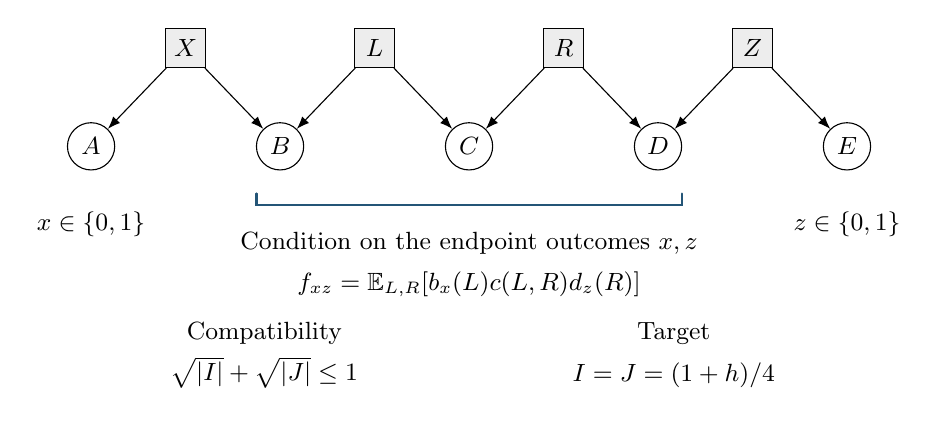
\begin{tikzpicture}[x=1cm,y=1cm]
\foreach \v/\x in {A/0,B/2.4,C/4.8,D/7.2,E/9.6}{\node[observer] (\v) at (\x,0) {$\v$};}
\foreach \s/\x/\a/\b in {X/1.2/A/B,L/3.6/B/C,R/6/C/D,Z/8.4/D/E}{
\node[source] (\s) at (\x,1.25) {$\s$};
\draw[causal] (\s)--(\a);\draw[causal] (\s)--(\b);
}
\node[font=\small,below=4mm of A] {$x\in\{0,1\}$};
\node[font=\small,below=4mm of E] {$z\in\{0,1\}$};
\draw[inkblue,line width=.8pt] (2.1,-.6)--(2.1,-.75)--(7.5,-.75)--(7.5,-.6);
\node[font=\small,align=center] at (4.8,-1.5) {Condition on the endpoint outcomes $x,z$\\[4pt]$f_{xz}=\mathbb E_{L,R}[b_x(L)c(L,R)d_z(R)]$};
\node[font=\small,align=center] at (2.2,-2.65) {Compatibility\\[4pt]$\sqrt{|I|}+\sqrt{|J|}\le1$};
\node[font=\small,align=center] at (7.4,-2.65) {Target\\[4pt]$I=J=(1+h)/4$};
\end{tikzpicture}
\caption{The five-observer path. Conditioning on $A=x$ and $E=z$ changes only the outer sources $X,Z$; the inner sources $L,R$ remain independent. This gives the bilocal inequality. The target violates it by $\sqrt{1+h}-1$ while retaining full support.}\label{fig:path}
\end{figure}


\subsubsection{The target}\label{sec:pathtarget}

\begin{definition}[Path target]\label{def:pathtarget}
For $0<h<1$ define the law $P_h$ by
\begin{equation}\label{eq:pathtarget}
P_h(x,b,c,d,z)=\frac1{32}\Bigl[1+bcd\,\frac{1+h}4\bigl(1+(-1)^{x+z}\bigr)\Bigr],
\qquad x,z\in\{0,1\},\ b,c,d\in\{-1,1\}.
\end{equation}
\end{definition}
\FloatBarrier

\begin{lemma}[Properties of $P_h$]\label{lem:pathtarget}
$P_h$ is a probability law, every atom is at least $(1-h)/64$, the pair $(A,E)$ consists of independent fair bits, every proper nonempty moment of $(B,C,D)$ conditional on $(A,E)$ vanishes, and
\begin{equation}\label{eq:fxz}
f_{xz}:=\E\bigl[BCD\mid A=x,E=z\bigr]=\frac{1+h}4\bigl(1+(-1)^{x+z}\bigr)
=\begin{cases}(1+h)/2,&x=z,\\0,&x\ne z.\end{cases}
\end{equation}
\end{lemma}

\begin{proof}
The bracket in \eqref{eq:pathtarget} lies between $1-(1+h)/2=(1-h)/2$ and $1+(1+h)/2$, so every atom lies in $[(1-h)/64,\,(3+h)/64]$ and in particular is positive. Summing $bcd$ over $\{-1,1\}^3$ gives zero, so the atoms sum to $32\cdot\frac1{32}=1$ and the $(A,E)$ marginal is uniform on four cells. Given $(x,z)$, the conditional density of $(b,c,d)$ is $\frac18\bigl[1+bcd\,f_{xz}\bigr]$, whose only nonvanishing nontrivial character is $bcd$, with value $f_{xz}$; that is \eqref{eq:fxz} and the vanishing of the proper moments.
\end{proof}

\subsubsection{A bilocal obstruction}\label{sec:bilocal}

\begin{lemma}[Bilocal inequality on the path]\label{lem:bilocal}
Let $R\in\Cpath$ with $R(A=x,E=z)>0$ for all four $(x,z)$, put $f_{xz}=\E_R[BCD\mid A=x,E=z]$ and
\[
I=\frac14\sum_{x,z}f_{xz},\qquad J=\frac14\sum_{x,z}(-1)^{x+z}f_{xz}.
\]
Then $\sqrt{|I|}+\sqrt{|J|}\le1$.
\end{lemma}

\begin{proof}
Absorb the response seeds into incident sources. Conditioning on $\{A=x\}$ reweights the law of $X$ alone, and conditioning on $\{E=z\}$ reweights the law of $Z$ alone, so under the conditional law $X,L,R,Z$ are still mutually independent, and $L,R$ keep their original laws. Writing
\[
b_x(\ell)=\E\bigl[B\mid L=\ell,\ A=x\bigr],\qquad
d_z(\rho)=\E\bigl[D\mid R=\rho,\ E=z\bigr],
\]
\[
c(\ell,\rho)=\E\bigl[C\mid L=\ell,\ R=\rho\bigr],
\]
all with values in $[-1,1]$, conditional independence of the three responses given the sources gives
\[
f_{xz}=\E_{L,R}\bigl[b_x(L)\,c(L,R)\,d_z(R)\bigr].
\]
Put $\beta_\pm=\tfrac12(b_0\pm b_1)$ and $\delta_\pm=\tfrac12(d_0\pm d_1)$. Then
\[
I=\E_{L,R}\bigl[\beta_+(L)\,c(L,R)\,\delta_+(R)\bigr],\qquad
J=\E_{L,R}\bigl[\beta_-(L)\,c(L,R)\,\delta_-(R)\bigr],
\]
so, using $|c|\le1$ and the independence of $L$ and $R$,
\[
|I|\le p_+r_+,\qquad |J|\le p_-r_-,\qquad
p_\pm=\E_L|\beta_\pm|,\quad r_\pm=\E_R|\delta_\pm| .
\]
For real $u,v$ with $|u|,|v|\le1$,
$\bigl|\tfrac{u+v}2\bigr|+\bigl|\tfrac{u-v}2\bigr|=\max(|u|,|v|)\le1$,
so $p_++p_-\le1$ and $r_++r_-\le1$. Cauchy--Schwarz gives
\[
\sqrt{|I|}+\sqrt{|J|}\le\sqrt{p_+r_+}+\sqrt{p_-r_-}\le\sqrt{p_++p_-}\,\sqrt{r_++r_-}\le1 . \qedhere
\]
\end{proof}

Inequalities of this shape originate with Branciard, Rosset, Gisin and Pironio \cite{BranciardRossetGisinPironio2012} for the bilocal scenario with measurement inputs; Lemma~\ref{lem:bilocal} is the specialization to a single fixed setting, one binary central output and two binary endpoint observations, proved here for arbitrary latent alphabets and stochastic responses.

\begin{corollary}[Quantitative incompatibility]\label{cor:pathdistance}
For every $0<h<1$,
\[
P_h\notin\Cpath\qquad\text{and}\qquad d_{\TV}(P_h,\Cpath)\ \ge\ \frac h{96}.
\]
\end{corollary}

\begin{proof}
By \eqref{eq:fxz}, $I=J=(1+h)/4$ for $P_h$, so $\sqrt I+\sqrt J=\sqrt{1+h}>1$ and Lemma~\ref{lem:bilocal} rules out compatibility.

Let $R\in\Cpath$ and $d=d_{\TV}(P_h,R)$. If $d\ge1/8$ then $d>1/96>h/96$, so assume $d<1/8$. Each endpoint cell satisfies $|R(x,z)-\tfrac14|\le d$, hence $R(x,z)\ge\tfrac14-d>\tfrac18>0$ and Lemma~\ref{lem:bilocal} applies to $R$. Write $N_R(x,z)=\E_R\bigl[BCD\,\one\{A=x,E=z\}\bigr]$ and $N_P$ for the same quantity under $P_h$, so $f^R_{xz}=N_R(x,z)/R(x,z)$ and likewise for $P_h$. The eight atoms of one endpoint cell contribute at most $2d$ to $\sum|R-P_h|$, so $|N_R-N_P|\le2d$, while $|R(x,z)-P_h(x,z)|\le d$. Since $|N_P|\le P_h(x,z)=\tfrac14$,
\[
\bigl|f^R_{xz}-f^P_{xz}\bigr|
\le\frac{|N_R-N_P|}{R(x,z)}+\frac{|N_P|\,\bigl|P_h(x,z)-R(x,z)\bigr|}{R(x,z)P_h(x,z)}
\le\frac{2d+d}{R(x,z)}\le24d .
\]
Averaging, $|I_R-I_P|\le24d$ and $|J_R-J_P|\le24d$. If $24d<h/4$ then
$I_R,J_R>\tfrac{1+h}4-\tfrac h4=\tfrac14$, so $\sqrt{|I_R|}+\sqrt{|J_R|}>1$, contradicting Lemma~\ref{lem:bilocal}. Hence $24d\ge h/4$.
\end{proof}

\subsubsection{The witness at every order}\label{sec:pathwitness}

\begin{theorem}[The path at every order]\label{thm:fivepath}
For every $t\ge1$ put $\gamma=1/(4t)$ and $h_t=\gamma^2=1/(16t^2)$. Then
\[
P_{h_t}\in\Iexp_t(P_5)=\IAI_t(P_5),\qquad P_{h_t}\notin\Cpath ,
\]
with a strictly positive rational target and a rational witness. Consequently $\tmin^H(P_{h_t})>t$ for $H\in\{\mathrm{NW},\mathrm{AI},\mathrm{exp}\}$, no finite order of any of the three hierarchies characterizes $\Cpath$, and
\[
d_{\TV}(P_{h_t},\Cpath)\ \ge\ \frac1{1536\,t^2}.
\]
\end{theorem}

\begin{proof}
\emph{The auxiliary law.} On signs $u=(u_1,\dots,u_t)$ and $v=(v_1,\dots,v_t)$ set
\begin{equation}\label{eq:Ht}
H_t(u,v)=2^{-2t}\,\Real\Bigl[\prod_{i=1}^t(1+i\gamma u_i)\prod_{j=1}^t(1-i\gamma v_j)\Bigr].
\end{equation}
Writing $\sigma=(u_1,\dots,u_t,-v_1,\dots,-v_t)\in\{-1,1\}^{2t}$, the bracket is $\prod_{k=1}^{2t}(1+i\gamma\sigma_k)$, whose real part keeps the even characters with coefficient $(i\gamma)^{|S|}=(-h_t)^{|S|/2}$, so
\[
H_t=2^{-2t}\sum_{\substack{S\subseteq[2t]\\|S|\text{ even}}}(-h_t)^{|S|/2}\prod_{k\in S}\sigma_k .
\]
This is $H_{2t,h_t}$ of Lemma~\ref{lem:parityaux} read in the coordinates $\sigma$, and $(2t)^2h_t=1/4$, so $H_t$ is a probability law with
\begin{equation}\label{eq:Htpos}
H_t(u,v)\ \ge\ \tfrac23\,2^{-2t}\ >\ 0 .
\end{equation}
All its values are rational.

\emph{The witness.} Draw $(u,v)\sim H_t$; independently draw fair bits $X_a$ and $Z_e$, fair signs $r_i$ and $s_j$, and fair signs $\nu_{ij}$, all mutually independent, $a,i,j,e\in[t]$. With $u^0=1$ and $u^1=u$, define every copied observation by
\begin{equation}\label{eq:pathwitness}
A^a=X_a,\qquad
B^{ai}=r_i\,u_i^{X_a},\qquad
C^{ij}=\begin{cases}r_is_j,&u_i=v_j,\\ r_is_j\nu_{ij},&u_i\ne v_j,\end{cases}\qquad
D^{je}=s_j\,v_j^{Z_e},\qquad
E^e=Z_e .
\end{equation}
Each copied observation is a function of the data attached to its copied parents together with its own private sign: $r_i$ and $u_i$ belong to $L_i$, and $s_j$ and $v_j$ to $R_j$. Call the resulting law $\Gamma_t$. It is a nonnegative rational probability law; the auxiliary density is strictly positive, while the observed table can have zero entries. As in Section~\ref{sec:construction}, $\Gamma_t$ is a law on the copied observations and not the output of an inflated model: under $H_t$ the families $u$ and $v$ are correlated.

\emph{Formal weights.} Give each $u_i$ the complex weight $(1+i\gamma u_i)/2$ and each $v_j$ the weight $(1-i\gamma v_j)/2$, and keep the actual probabilities of $X,Z,r,s,\nu$. Write $\E_\ast$ for the resulting formal expectation, a product functional on the $6t+t^2$ auxiliary coordinates, with $\E_\ast u_i=i\gamma$ and $\E_\ast v_j=-i\gamma$. Since the weights of the auxiliary coordinates multiply to a complex number whose real part is $H_t$, and the other coordinates carry real weights,
\begin{equation}\label{eq:realpart}
\E_{\Gamma_t}[F]=\Real\,\E_\ast[F]\qquad\text{for every real-valued }F .
\end{equation}

\emph{Every copied path has law $P_h$.} Fix $(a,i,j,e)$ and condition on $X_a=x$, $Z_e=z$, which are fair and independent and reproduce the $(A,E)$ marginal of $P_h$. The masks $r_i$ and $s_j$ are fair signs independent of everything else and each occurs in exactly one of $B^{ai}$, $D^{je}$ and in $C^{ij}$, so every product of a proper nonempty subset of $\{B^{ai},C^{ij},D^{je}\}$ carries $r_i$ or $s_j$ to an odd power and has formal expectation zero. In the triple product the masks cancel:
\[
B^{ai}C^{ij}D^{je}=u_i^{\,x}\,v_j^{\,z}\cdot\bigl(\one\{u_i=v_j\}+\nu_{ij}\one\{u_i\ne v_j\}\bigr),
\]
and $\E_\ast\nu_{ij}=0$, so $\E_\ast\bigl[B^{ai}C^{ij}D^{je}\bigr]=\E_\ast\bigl[u_i^{\,x}v_j^{\,z}\one\{u_i=v_j\}\bigr]$. The formal weight of $(u_i,v_j)=(+1,+1)$ is $\frac{1+i\gamma}2\cdot\frac{1-i\gamma}2=\frac{1+h}4$, and the weight of $(-1,-1)$ is the same real number, so
\[
\E_\ast\bigl[u_i^{\,x}v_j^{\,z}\one\{u_i=v_j\}\bigr]=\frac{1+h}4\bigl(1+(-1)^{x+z}\bigr)=f_{xz},
\]
which is real. Every character of the copied path is thus one of: a character of the fair bits $X_a,Z_e$ alone; a character carrying a proper nonempty subset of $\{B^{ai},C^{ij},D^{je}\}$, with formal expectation zero; or a character carrying all three, with formal expectation $\frac14\sum_{x,z}\chi(x,z)f_{xz}$. All of these are real and all agree with the corresponding characters of $P_h$ in Lemma~\ref{lem:pathtarget}, so by \eqref{eq:realpart}
\[
\Law_{\Gamma_t}\bigl(A^a,B^{ai},C^{ij},D^{je},E^e\bigr)=P_h,
\]
and $\E_\ast[G]$ is real for every function $G$ of a copied path.

\emph{Injectable marginals.} An injectable set of the path contains at most one copied observation over each of $A,B,C,D,E$ and its copy indices agree on shared sources, so it lies in a copied path $(a,i,j,e)$ with consistent indices, after completing unused indices arbitrarily. Its marginal is therefore the corresponding marginal of $P_h$, and $\E_\ast[G]$ is real for every function $G$ of it.

\emph{Ancestral products and the diagonal law.} Let $F_1,\dots,F_r$ be pairwise ancestrally independent injectable sets. Distinct copied sources carry distinct auxiliary coordinates and distinct masks, and distinct copied observations carry distinct private signs, so the $F_k$ depend on disjoint coordinate families and $\E_\ast\bigl[\prod_k G_k\bigr]=\prod_k\E_\ast[G_k]$ for functions $G_k$ of $F_k$. Each factor is real by the previous paragraph, hence so is the product, and \eqref{eq:realpart} gives
\[
\E_{\Gamma_t}\Bigl[\prod_kG_k\Bigr]=\prod_k\E_\ast[G_k]=\prod_k\E_{\Gamma_t}[G_k].
\]
Taking the $G_k$ to be indicators of atoms shows the blocks are independent with the prescribed marginals. The diagonal rows $(A^\ell,B^{\ell\ell},C^{\ell\ell},D^{\ell\ell},E^\ell)$, $\ell\in[t]$, are pairwise ancestrally independent injectable copied paths, so the diagonal law is $P_h^{\otimes t}$.

\emph{Symmetry.} The density \eqref{eq:Ht} is symmetric in $u_1,\dots,u_t$ and in $v_1,\dots,v_t$ separately, the families $(X_a)$, $(Z_e)$, $(r_i)$, $(s_j)$ and $(\nu_{ij})$ are i.i.d., and \eqref{eq:pathwitness} is equivariant, so $\Gamma_t$ is invariant under independent permutations of the four copy-index families. Together with the previous two paragraphs this places $P_{h_t}$ in $\IAI_t(P_5)$, and Lemma~\ref{lem:rootsink} gives $\Iexp_t(P_5)=\IAI_t(P_5)$.

\emph{Conclusion.} Corollary~\ref{cor:pathdistance} gives $P_{h_t}\notin\Cpath$ and
$d_{\TV}(P_{h_t},\Cpath)\ge h_t/96=1/(1536t^2)$. Membership at order $t$ forces $\tmin^H(P_{h_t})>t$ for each of the three hierarchies, by Proposition~\ref{prop:gsound}.
\end{proof}

Along this family the first rejecting order grows without bound while the target stays uniformly inside the simplex: since $h_t\le1/16$, Lemma~\ref{lem:pathtarget} gives
\[
P_{h_t}(x,b,c,d,z)\ \ge\ \frac{1-h_t}{64}\ \ge\ \frac{15}{1024}
\]
for every $t$ and every atom. The obstruction therefore does not come from vanishing probabilities. The theorem supplies a distance lower bound of order $t^{-2}$; it does not determine this family's distance asymptotics. The general upper bound is $O(t^{-1/2})$. Whether the path admits accepted laws at distance $\Omega(t^{-1})$, as the triangle and square do, remains open.


\section{Quantitative convergence on the triangle and square}\label{sec:cyclequant}

Section~\ref{sec:classification} proves the classification. We now measure the gap between finite-order feasibility and compatibility on the triangle and square. The parity witness of Section~\ref{sec:cycles} gives an initial lower bound; a modification of its unconstrained Fourier coefficients improves it to $\Omega(1/t)$. A convex-order argument supplies the upper bound, and the final two subsections compare the hierarchy orders and finite thresholds.

\subsection{A corrected density and a linear lower bound}\label{sec:corrected}

The density \eqref{eq:Hdensity} fixes every auxiliary character, including characters that no prescription refers to. Changing those characters restores positivity at a larger $q$.

\begin{lemma}[Phase telescoping]\label{lem:telescope}
For real $\theta_1,\dots,\theta_m$,
\[
1-\cos\Bigl(\sum_{g=1}^m\theta_g\Bigr)\ \le\ m\sum_{g=1}^m\bigl(1-\cos\theta_g\bigr).
\]
\end{lemma}

\begin{proof}
$1-\cos\phi=\tfrac12|1-e^{i\phi}|^2$, and
$1-\prod_ge^{i\theta_g}=\sum_g\bigl(\prod_{g'<g}e^{i\theta_{g'}}\bigr)(1-e^{i\theta_g})$,
so $|1-\prod_ge^{i\theta_g}|\le\sum_g|1-e^{i\theta_g}|$. Cauchy--Schwarz gives $\bigl(\sum_g a_g\bigr)^2\le m\sum_ga_g^2$.
\end{proof}

\begin{lemma}[Corrected density]\label{lem:corrected}
Fix $m\in\{3,4\}$, $t\ge1$ and $0<q\le1/(16t)$, and set $c=4$ for $m=3$ and $c=5$ for $m=4$. On $m$ families of $t$ signs $s_{g,i}$ put
\begin{equation}\label{eq:Wdensity}
f_g=\prod_{i=1}^t\bigl(1+\mathrm{i}\sqrt q\,s_{g,i}\bigr),\qquad R=(1+q)^{t/2},\qquad
W(s)=\Real\prod_{g=1}^mf_g+c\sum_{g=1}^m\bigl(1-\Real f_g\bigr).
\end{equation}
Then $W$ is a real polynomial in $q$ with rational coefficients, $W\ge3/5$ for $m=3$ and $W\ge1/3$ for $m=4$, the law $\rho=2^{-mt}W$ is a probability law, and its characters are
\begin{equation}\label{eq:Wmoments}
\E_\rho\Bigl[\prod_{w\in S}s_w\Bigr]=
\begin{cases}
0,&|S|\text{ odd},\\
(1-c)(-q)^{|S|/2},&S\ne\varnothing\text{ even, inside one family},\\
(-q)^{|S|/2},&|S|\text{ even, meeting at least two families}.
\end{cases}
\end{equation}
\end{lemma}

\begin{proof}
Here $\mathrm{i}^2=-1$. Taking real parts keeps only even powers of $\mathrm{i}\sqrt q$, so $W$ is a real polynomial in $q$. Since $|1+i\sqrt q\,s|=(1+q)^{1/2}$ we may write $f_g=Re^{i\theta_g}$, and then
\[
\begin{aligned}
W&=R^m\cos\Bigl(\sum_g\theta_g\Bigr)+c\sum_g\bigl(1-R\cos\theta_g\bigr)\\
&=R^m-cm(R-1)-R^m\Bigl(1-\cos\sum_g\theta_g\Bigr)+cR\sum_g\bigl(1-\cos\theta_g\bigr).
\end{aligned}
\]
Lemma~\ref{lem:telescope} gives
\[
W\ \ge\ R^m-cm(R-1)+\bigl(cR-mR^m\bigr)\sum_g\bigl(1-\cos\theta_g\bigr).
\]
From $tq\le1/16$ we get $R^2=(1+q)^t\le\sum_{j\ge0}(tq)^j\le16/15$ and $R-1=(R^2-1)/(R+1)\le1/30$. For $m=3$, $c=4$: $3R^3\le4R$ because $3R^2\le16/5\le4$, and $W\ge1-12/30=3/5$. For $m=4$, $c=5$: $4R^4\le5R$ because $4R^3\le4(16/15)^{3/2}<5$, and $W\ge1-20/30=1/3$.

For the characters, work under the uniform law on the sign cube, where the families are independent and $\E f_g=1$. For $S$ with parts $S_g$ in the families,
\[
\E\Bigl[\prod_gf_g\prod_{w\in S}s_w\Bigr]=\prod_g\E\Bigl[f_g\prod_{w\in S_g}s_w\Bigr]=(i\sqrt q)^{|S|},
\]
whose real part is $0$ for odd $|S|$ and $(-q)^{|S|/2}$ for even $|S|$. Also $\E[(1-\Real f_g)\prod_{w\in S}s_w]$ vanishes unless $S$ is a nonempty subset of family $g$, in which case it equals $-\Real(i\sqrt q)^{|S|}$. Adding the contributions gives \eqref{eq:Wmoments}; the case $S=\varnothing$ gives $\E_\rho1=1$.
\end{proof}

\begin{theorem}[The square at $q=\Theta(1/t)$]\label{thm:squarelinear}
For every $t\ge1$ and every $0<q\le1/(16t)$, the square parity law $P_q$ of \eqref{eq:squaretarget} lies in $\IAI_t(\square)=\Iexp_t(\square)$.
\end{theorem}

\begin{proof}
Take $m=4$ and $c=5$ in Lemma~\ref{lem:corrected}, name the four families $x,y,z,w$ after the sources $X,Y,Z,W$, and define every copied observation by
\[
A^{il}=x_iw_l,\qquad B^{ij}=x_iy_j,\qquad C^{jk}=y_jz_k,\qquad D^{kl}=z_kw_l,
\]
that is by \eqref{eq:cyclewitness} for $m=4$. The density \eqref{eq:Wdensity} is symmetric within each family, so the law is invariant under independent permutations of the copy indices of each source. By Lemma~\ref{lem:boundary} every boundary occurring in an AI prescription, and every boundary of a subset of one of its blocks, is empty or meets at least two families; by \eqref{eq:Wmoments} such characters take the value $(-q)^{|\partial\cdot|/2}$, unchanged from \eqref{eq:masterchar}. The computation of Lemma~\ref{lem:cyclewitness} therefore applies verbatim: every injectable set has the marginal of $P_{4,q}=P_q$, ancestrally independent injectable blocks are independent, and the diagonal law is $P_q^{\otimes t}$. The moments that Lemma~\ref{lem:corrected} changed are the nonempty even characters inside a single family, and no prescription refers to one. Lemma~\ref{lem:rootsink} gives the recursive prescriptions.
\end{proof}

\begin{theorem}[The triangle at $q=\Theta(1/t)$]\label{thm:trianglelinear}
For every $t\ge1$ and every $0<q\le1/(16t)$, the parity-even law $\Pi(-q,-q,-q)$ of \eqref{eq:paritylaw} lies in $\IAI_t(\triangle)=\Iexp_t(\triangle)$.
\end{theorem}

\begin{proof}
Take $m=3$ and $c=4$ in Lemma~\ref{lem:corrected}, name the three families $x,y,z$ after the sources $X,Y,Z$, and define
\[
A^{ij}=x_iz_j,\qquad B^{ik}=x_iy_k,\qquad C^{jk}=z_jy_k,
\]
which is \eqref{eq:cyclewitness} for $m=3$ in the index convention of Section~\ref{sec:triangle}. Positivity and normalization are Lemma~\ref{lem:corrected} with $W\ge3/5$. Symmetry within each family is again immediate. By Lemma~\ref{lem:boundary} every character prescribed by an injectable marginal, by an ancestrally independent product, or by the diagonal law has boundary empty or meeting at least two families, so \eqref{eq:Wmoments} returns $(-q)^{|\partial\cdot|/2}$ and the argument of Lemma~\ref{lem:cyclewitness} applies unchanged. The original copied triangle has $\E A=\E[x_iz_j]=-q$ and likewise $\E B=\E C=-q$, while $ABC=x_iz_jx_iy_kz_jy_k=1$, so its law is $\Pi(-q,-q,-q)=P_{3,q}$. Lemma~\ref{lem:rootsink} gives the recursive prescriptions.
\end{proof}
\subsection{Distance and the worst-case profile}\label{sec:worstcase}

For $H\in\{\mathrm{NW},\mathrm{AI},\mathrm{exp}\}$ and a pair-source scenario $G$ set
\begin{equation}\label{eq:Hprofile}
H^H_t(G)=\sup_{P\in\mathcal I^H_t(G)}d_{\TV}(P,\Cscen{G}),
\end{equation}
the worst-case total-variation distance from compatibility of a law the order-$t$ test accepts, with $d_{\TV}$ half the $\ell^1$ distance as in Section~\ref{sec:setup}.

\begin{lemma}[Max-moment inequality for the square]\label{lem:maxmoment}
Every $P\in\Csq$ in sign notation satisfies
\[
\max\{\E A,\ \E B,\ \E[AB]\}+4\,P(ABCD=-1)\ \ge\ 0 .
\]
\end{lemma}

\begin{proof}
Absorb the response seeds into incident sources, so $A=A(X,W)$, $B=B(X,Y)$, $C=C(Y,Z)$, $D=D(Z,W)$ are deterministic signs and $X,Y,Z,W$ are independent. Fix $z$ and write $g_z(Y)=C(Y,z)$, $h_z(W)=D(z,W)$ and
\[
\delta_z=\Pr\bigl(A(X,W)B(X,Y)\ne g_z(Y)h_z(W)\bigr),
\]
so that $\E_Z\delta_Z=P(ABCD=-1)=:\delta$. Put
\[
u_z(x)=\E_W\bigl[A(x,W)h_z(W)\bigr],\qquad v_z(x)=\E_Y\bigl[B(x,Y)g_z(Y)\bigr].
\]
Since $Y$ and $W$ are independent, $\E[ABg_zh_z\mid X=x]=u_z(x)v_z(x)$, and as $ABg_zh_z$ is a sign, $\E_X[1-u_zv_z]=2\delta_z$.

Let $f_z(x)=\sgn(u_z(x)+v_z(x))$, with $\sgn0=1$, and compare $A$ and $B$ with $A'_z=f_z(X)h_z(W)$ and $B'_z=f_z(X)g_z(Y)$. Then
\[
e_z:=\Pr(A\ne A'_z)+\Pr(B\ne B'_z)=\E_X\Bigl[1-\tfrac12|u_z+v_z|\Bigr]\le\E_X\bigl[1-u_zv_z\bigr]=2\delta_z,
\]
using $|u+v|\ge2uv$ on $[-1,1]^2$. Independence of $X,Y,W$ gives
\[
(\E A'_z)(\E B'_z)(\E[A'_zB'_z])=(\E f_z)^2(\E g_z)^2(\E h_z)^2\ \ge\ 0,
\]
so at least one of the three comparison moments is nonnegative. Each differs from the corresponding moment of $P$ by at most $2e_z$, since $|\E U-\E V|\le2\Pr(U\ne V)$ for signs and $\Pr(AB\ne A'_zB'_z)\le\Pr(A\ne A'_z)+\Pr(B\ne B'_z)$. Hence
\[
\max\{\E A,\E B,\E[AB]\}\ \ge\ -2e_z\ \ge\ -4\delta_z .
\]
The left side does not depend on $z$; averaging over $z$ finishes the proof.
\end{proof}

\begin{corollary}[Full-support survivors on the square]\label{cor:squaredistance}
$d_{\TV}(P_q,\Csq)\ge q/6$ for $0<q\le3-2\sqrt2$. With flip probability $\eta=q/64$ applied to each of the four bits and to every copied observation, $\widetilde P_q=T_\eta^{\otimes4}P_q$ is strictly positive, lies in $\IAI_t(\square)=\Iexp_t(\square)$ for $q\le1/(16t)$, and satisfies $d_{\TV}(\widetilde P_q,\Csq)\ge5q/48$. At $q_t=1/(16t)$,
\[
H^{\mathrm{exp}}_t(\square)=H^{\mathrm{AI}}_t(\square)\ \ge\ \frac5{768\,t}.
\]
\end{corollary}

\begin{proof}
If $R\in\Csq$ and $d=d_{\TV}(P_q,R)$, each of $\E_RA$, $\E_RB$, $\E_R[AB]$ is at most $-q+2d$ and the parity error of $R$ is at most $d$, since $P_q$ has none. Lemma~\ref{lem:maxmoment} gives $0\le-q+2d+4d$, so $d\ge q/6$. The noise argument of Theorem~\ref{thm:cycle} applies to the witness of Theorem~\ref{thm:squarelinear}, and $d_{\TV}(\widetilde P_q,P_q)\le4\eta=q/16$, so $d_{\TV}(\widetilde P_q,\Csq)\ge q/6-q/16=5q/48$. Substituting $q_t=1/(16t)$ gives $5/(768t)$, and Lemma~\ref{lem:rootsink} identifies the two suprema.
\end{proof}

\begin{corollary}[Full-support survivors on the triangle]\label{cor:triangledistance}
$d_{\TV}(\Pi(-q,-q,-q),\Ctri)\ge q/10$ for $0<q\le1/3$. With flip probability $\eta=q/192$ on each of the three bits and on every copied observation, the noisy target is strictly positive, lies in $\IAI_t(\triangle)=\Iexp_t(\triangle)$ for $q\le1/(16t)$, and is at distance at least $27q/320$ from $\Ctri$. At $q_t=1/(16t)$,
\[
H^{\mathrm{exp}}_t(\triangle)=H^{\mathrm{AI}}_t(\triangle)\ \ge\ \frac{27}{5120\,t}.
\]
\end{corollary}

\begin{proof}
The distance bound is Lemma~\ref{lem:cycledistance} for $m=3$, whose proof uses only Lemma~\ref{lem:quantrigidity} on the triangle itself. The three flips cost at most $3\eta=q/64$ in total variation, and $q/10-q/64=27q/320$. Feasibility is Theorem~\ref{thm:trianglelinear} with the noise argument of Theorem~\ref{thm:cycle}. Substituting $q_t=1/(16t)$ gives $27/(5120t)$.
\end{proof}

\subsection{A convex-order upper bound}\label{sec:convexorder}

Figure~\ref{fig:convex-order} summarizes the two ways of sampling a table used in the proof.

\begin{theorem}[Convex order along the diagonal]\label{thm:convexorder}
Let $G$ be a correlation scenario, that is, finitely many independent latent sources and observed variables with finite alphabets, each a stochastic function of the sources it reads, with $K$ joint outcomes; the order-$n$ inflation and the set $\INW_n(G)$ are defined as in Section~\ref{sec:pairsource} with sources in place of edges. Let $P\in\INW_n(G)$ with witness $\Gamma$. For a deterministic table $\omega$ of copied observations let $q_\omega$ be the observed law obtained by sampling one copy index uniformly and independently for each source and reading $\omega$ at those indices. Then $q_\omega\in\Cscen{G}$ for every $\omega$, and for every convex $\Phi$ on the observed simplex
\begin{equation}\label{eq:convexorder}
\E_\Gamma\,\Phi(q_\omega)\ \le\ \E\,\Phi(\widehat P_n),
\end{equation}
where $\widehat P_n$ is the empirical law of $n$ independent draws from $P$. In particular
\begin{equation}\label{eq:convexl2}
\E_\Gamma\|q_\omega-P\|_2^2\ \le\ \frac{1-\|P\|_2^2}{n},
\qquad
H^{\mathrm{NW}}_n(G)\ \le\ \min\Bigl\{1,\ \frac{\sqrt{K-1}}{2\sqrt n}\Bigr\}.
\end{equation}
\end{theorem}

\begin{proof}
Fix $\omega$. Sampling an index $I_e\in[n]$ uniformly and independently for each source $e$ and letting each observed variable $v$ output $\omega_v\bigl((I_e)_{e\ni v}\bigr)$, where $e\ni v$ ranges over the sources $v$ reads, is a model of $G$ with independent sources $I_e$ and deterministic responses, so $q_\omega\in\Cscen{G}$.

Draw one uniform permutation $\pi_e$ of $[n]$ for each source, independently of each other and of $\omega\sim\Gamma$, and set
\[
T_\ell=\Bigl(\omega_v\bigl((\pi_e(\ell))_{e\ni v}\bigr)\Bigr)_{v},\qquad \ell\in[n],
\qquad \widehat P=\frac1n\sum_{\ell=1}^n\delta_{T_\ell}.
\]
For each fixed choice of permutations, the symmetry of $\Gamma$ carries $(T_1,\dots,T_n)$ to the diagonal rows, so $(T_1,\dots,T_n)\sim P^{\otimes n}$; this remains true after averaging over the permutations, so $\widehat P$ has the law of $\widehat P_n$. Conditionally on $\omega$ and on a fixed $\ell$, the indices $(\pi_e(\ell))_e$ are independent and uniform on $[n]$, so $\E[\delta_{T_\ell}\mid\omega]=q_\omega$ and hence $\E[\widehat P\mid\omega]=q_\omega$. Conditional Jensen gives $\Phi(q_\omega)\le\E[\Phi(\widehat P)\mid\omega]$, and averaging over $\omega$ gives \eqref{eq:convexorder}.

Take $\Phi(\mu)=\|\mu-P\|_2^2$. Then $\E\|\widehat P_n-P\|_2^2=\frac1n\sum_xP(x)(1-P(x))=(1-\|P\|_2^2)/n$, which is the first part of \eqref{eq:convexl2}. Some $\omega$ attains at most the mean, and its $q_\omega$ is compatible, so
\[
d_{\TV}(P,\Cscen{G})\le\tfrac12\|P-q_\omega\|_1\le\frac{\sqrt K}2\|P-q_\omega\|_2\le\frac{\sqrt K}2\sqrt{\frac{1-\|P\|_2^2}n}\le\frac{\sqrt{K-1}}{2\sqrt n},
\]
using $\|P\|_2^2\ge1/K$. Total variation never exceeds $1$.
\end{proof}

\begin{figure}[!htbp]
\centering
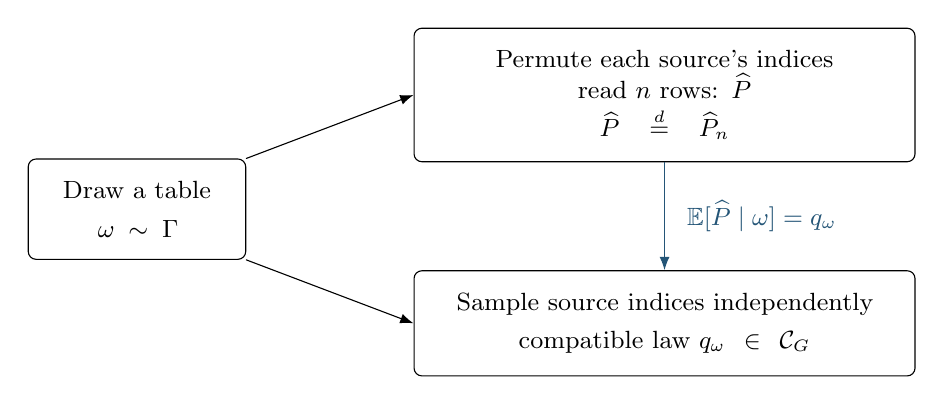
\begin{tikzpicture}[box/.style={draw,rounded corners=1mm,align=center,font=\small,inner sep=8pt,text width=5.8cm}]
\node[box,text width=2.2cm] (table) at (0,0) {Draw a table\\[3pt]$\omega\sim\Gamma$};
\node[box] (emp) at (6.7,1.45) {Permute each source's indices\\read $n$ rows: $\widehat P$\\[3pt]$\widehat P\overset{d}{=}\widehat P_n$};
\node[box] (comp) at (6.7,-1.45) {Sample source indices independently\\[3pt]compatible law $q_\omega\in\mathcal C_G$};
\draw[-{Latex}] (table.north east)--(emp.west);
\draw[-{Latex}] (table.south east)--(comp.west);
\draw[-{Latex},inkblue] (emp.south)--node[right=5pt,font=\small,fill=white,inner sep=3pt] {$\mathbb E[\widehat P\mid\omega]=q_\omega$}(comp.north);
\end{tikzpicture}
\caption{The conditional expectation behind the convex-order bound. The same table yields an empirical distribution through permuted diagonal rows and a compatible law through independent source indices. Conditional Jensen compares their convex functionals. Squared Euclidean distance then gives the source-count-independent bound.}\label{fig:convex-order}
\end{figure}


The sampling mechanism is that of the finite de Finetti estimate of \cite[Section 4.2 and eq.~(A7)]{NW2020}, which bounds the same quantity by $L(1-\|P\|_2^2)/n$ for $L$ sources through the collision probability of two index samples. Using the full diagonal law through a conditional expectation, rather than its first two degrees, removes the factor $L$. Section~\ref{sec:general} draws the rejecting-order consequence.

\FloatBarrier
\begin{corollary}[Brackets for the square and the triangle]\label{cor:brackets}\label{thm:brackets-intro}
For every $t\ge1$,
\[
\frac5{768\,t}\ \le\ H^{\mathrm{exp}}_t(\square)=H^{\mathrm{AI}}_t(\square)\ \le\ H^{\mathrm{NW}}_t(\square)\ \le\ \min\Bigl\{1,\frac{\sqrt{15}}{2\sqrt t}\Bigr\},
\]
\[
\frac{27}{5120\,t}\ \le\ H^{\mathrm{exp}}_t(\triangle)=H^{\mathrm{AI}}_t(\triangle)\ \le\ H^{\mathrm{NW}}_t(\triangle)\ \le\ \frac{\sqrt7}{2\sqrt t}.
\]
\end{corollary}

\begin{proof}
Combine Corollaries~\ref{cor:squaredistance} and~\ref{cor:triangledistance} with Theorem~\ref{thm:convexorder} at $K=16$ and $K=8$, and with Proposition~\ref{prop:gsound}.
\end{proof}

The gap between $t^{-1}$ and $t^{-1/2}$ remains open for both scenarios (Question~\ref{q:hausdorff}).

\subsection{Order conversion on the square}\label{sec:conversion}

\begin{theorem}[NW and AI differ by a bounded change of order]\label{thm:orderconversion}
For every $t\ge2$,
\[
\INW_{\lfloor3t/2\rfloor}(\square)\ \subseteq\ \IAI_t(\square)=\Iexp_t(\square)\ \subseteq\ \INW_t(\square).
\]
\end{theorem}

The proof in Appendix~\ref{app:conversion} places the components of an AI set on at most $\lfloor3t/2\rfloor$ diagonal rows.

Hence $H^{\mathrm{NW}}_{\lfloor3t/2\rfloor}(\square)\le H^{\mathrm{AI}}_t(\square)\le H^{\mathrm{NW}}_t(\square)$, so the two hierarchies have the same polynomial decay exponent if either has one.

\subsection{Finite-order separation}\label{sec:lowthresholds}

For the square parity family $P_q$ and the triangle family $\Pi(-q,-q,-q)$, the accepted parameters at order $t$ form an interval $[0,q_t^H]$ (Lemma~\ref{lem:paritymonotone}). Rational certificates bracket the endpoints through order ten and separate the tests at the following orders.

\begin{proposition}[The parity thresholds at orders up to ten]\label{prop:paritythresholds}
For the square and the triangle, the thresholds $q^{\mathrm{AI}}_t=q^{\mathrm{exp}}_t$ and $q^{\mathrm{NW}}_t$ satisfy Table~\ref{tab:thresholds} for $1\le t\le10$. In particular:
\begin{enumerate}[label=(\roman*),nosep]
\item $q^{\mathrm{AI}}_t<q^{\mathrm{NW}}_t$ at every even $t\le10$, so $\IAI_t\subsetneq\INW_t$ at those orders on both scenarios;
\item the certified brackets agree at every odd $t\le9$; agreement of brackets does not establish equality of thresholds;
\item $q^{\mathrm{NW}}_{t+1}<q^{\mathrm{AI}}_t$ for $2\le t\le9$, $t\ne3$, on both scenarios, whereas the brackets at orders three (AI) and four (NW) agree;
\item on the square, $P_{3/20}\in\INW_2\setminus\IAI_2$ and $P_{1/10}\in\IAI_2\setminus\INW_3$.
\end{enumerate}
Consequently $\INW_3(\square)\subsetneq\IAI_2(\square)=\Iexp_2(\square)\subsetneq\INW_2(\square)$.
\end{proposition}

The proof is in Appendix~\ref{app:quantitative}. Figure~\ref{fig:thresholds} plots $tq_t^H$.

\begin{figure}[!htbp]
\centering
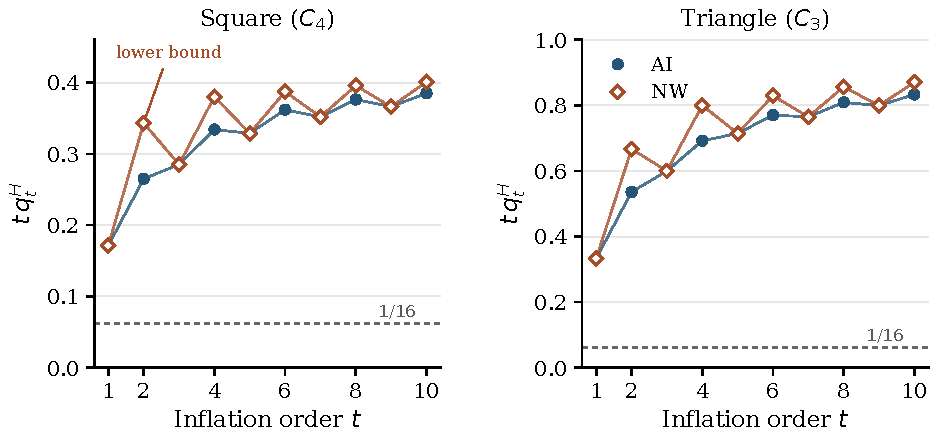
\includegraphics[width=.94\linewidth]{figures/thresholds.pdf}
\caption{Certified parity thresholds through order ten, rescaled by $t$. Markers show lower endpoints; two-sided brackets have width $4\cdot10^{-9}$ before rescaling. The square NW order-two point is a lower bound only. Dashed: the all-order guarantee $q=1/(16t)$ from Theorems~\ref{thm:squarelinear} and~\ref{thm:trianglelinear}. Panels use different vertical scales; connecting segments guide the eye.}\label{fig:thresholds}
\end{figure}


\section{The defect family and rejecting-order growth}\label{sec:main}

The parity laws of Sections~\ref{sec:cycles} and~\ref{sec:cyclequant} establish nontermination and worst-case lower bounds. We now study a second triangle family for which passing and rejecting bounds yield the same exponent, and the distance to compatibility can be computed to leading order.

For $0<\eps<1$ and $0\le r\le1$ define the three-bit law
\begin{equation}\label{eq:Q}
Q(\eps,r)=\eps\,\delta_{000}+(1-\eps)\,\Bern(r)^{\otimes3},
\end{equation}
a point mass at $000$ with weight $\eps$ mixed with three independent bits that equal $1$ with probability $r$. Throughout, $\Bern(r)$ denotes the law on $\{0,1\}$ with $\Bern(r)(1)=r$.

\begin{theorem}[Membership at every finite order]\label{thm:membership}
Let $t\ge1$, $0<\eps<1$ and $0\le r\le(1-\eps)^{t-1}$. Then
\[
Q(\eps,r)\in\Iexp_t\subseteq\IAI_t\subseteq\INW_t.
\]
\end{theorem}

\begin{theorem}[No finite characterizing order]\label{thm:main}\label{thm:main-intro}
For every integer $t\ge1$, with $\eps_t=1/(2t^3)$ and $r_t=(1-\eps_t)^{t-1}$, the law $P_t=Q(\eps_t,r_t)$ satisfies
\[
P_t\in\Iexp_t\subseteq\IAI_t\subseteq\INW_t
\qquad\text{and}\qquad
P_t(000)^2-P_{t,A}(0)P_{t,B}(0)P_{t,C}(0)\ \ge\ \frac{\eps_t^2}{2}\ >0,
\]
so $P_t\notin\Ctri$. Hence none of the three finite-order tests characterizes $\Ctri$ at any finite order.
\end{theorem}

Theorem~\ref{thm:main} includes $t=1$, where $P_1=\tfrac12(\delta_{000}+\delta_{111})$, the perfectly correlated three-bit law, which is the standard example of a triangle-incompatible distribution and passes the trivial order-one test.

\begin{corollary}[Larger alphabets]\label{cor:alphabets}
For the triangle with observed alphabets of any sizes $n_A,n_B,n_C\ge2$, no finite order of the Navascués--Wolfe hierarchy characterizes the compatible set.
\end{corollary}
\begin{proof}
The binary-support transfer in Remark~\ref{rem:alphabets} applies to $P_t$ and its inflation witness.
\end{proof}


\subsection{The defect cube}\label{sec:construction}

Fix $t\ge1$, $0<\eps<1$ and $0\le r\le(1-\eps)^{t-1}$. The witness is a joint law $\Gamma_t$ on the $3t^2$ copied observations built from independent bits indexed by the cells of the cube $[t]^3$.

\paragraph{Roots.}
Let $D_{ijk}\sim\Bern(\eps)$, $(i,j,k)\in[t]^3$, be mutually independent \emph{defect} bits, and let $N_v\sim\Bern(s)$, one for each copied observation $v$, be mutually independent \emph{private} bits, independent of the defects, with
\begin{equation}\label{eq:s}
s=1-\frac{r}{(1-\eps)^{t-1}}\in[0,1].
\end{equation}
The endpoint $r=0$ uses $s=1$; the endpoint $r=(1-\eps)^{t-1}$ uses $s=0$, in which case the private bits play no role.

\paragraph{Outputs.}
Define
\begin{equation}\label{eq:outputs}
\begin{aligned}
A^{ij}&=\one\bigl\{N_{A^{ij}}=0\text{ and }D_{ijk}=0\ \forall k\bigr\},\\
B^{ik}&=\one\bigl\{N_{B^{ik}}=0\text{ and }D_{ijk}=0\ \forall j\bigr\},\\
C^{jk}&=\one\bigl\{N_{C^{jk}}=0\text{ and }D_{ijk}=0\ \forall i\bigr\}.
\end{aligned}
\end{equation}
Figure~\ref{fig:defect-cube} shows the line geometry: $A^{ij}$ reads the line of cells $\Lambda(A^{ij})=\{(i,j,k):k\in[t]\}$, $B^{ik}$ the line $\Lambda(B^{ik})=\{(i,j,k):j\in[t]\}$, and $C^{jk}$ the line $\Lambda(C^{jk})=\{(i,j,k):i\in[t]\}$; each output equals $1$ exactly when its private bit and every defect on its line are $0$. Let $\Gamma_t$ be the joint law of the outputs. For $s=0$ its entries are
\begin{equation}\label{eq:table}
\Gamma_t(w)=\sum_{d\in\{0,1\}^{[t]^3}:\,F_t(d)=w}\eps^{|d|}(1-\eps)^{t^3-|d|}.
\end{equation}
For rational $\eps$, these entries are rational. Here $F_t$ is the map \eqref{eq:outputs} from defect configurations to observed assignments. The entries are nonnegative and sum to $(\eps+1-\eps)^{t^3}=1$.

$\Gamma_t$ does not come from running an inflated triangle model; it is a probability law on the copied observations, which is what a finite inflation test asks for.

\begin{figure}[!htbp]
\centering
\begin{minipage}[c]{.48\linewidth}
\centering
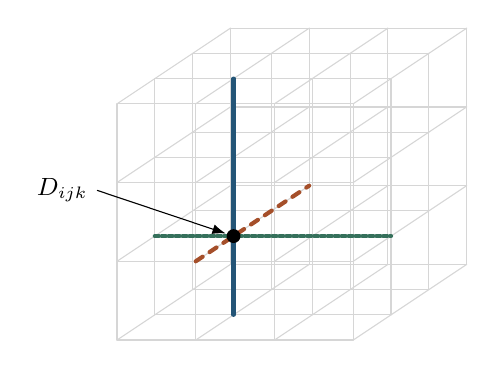
\begin{tikzpicture}[x={(1cm,0cm)},y={(.48cm,.32cm)},z={(0cm,1cm)}]
\foreach \x in {0,...,3}{\foreach \y in {0,...,3}{\draw[black!16,thin] (\x,\y,0)--(\x,\y,3);}}
\foreach \x in {0,...,3}{\foreach \z in {0,...,3}{\draw[black!16,thin] (\x,0,\z)--(\x,3,\z);}}
\foreach \y in {0,...,3}{\foreach \z in {0,...,3}{\draw[black!16,thin] (0,\y,\z)--(3,\y,\z);}}
\draw[inkblue,line width=1.5pt] (1,1,0)--(1,1,3);
\draw[inkrust,line width=1.5pt,dashed] (1,0,1)--(1,3,1);
\draw[inkgreen,line width=1.5pt,densely dotted] (0,1,1)--(3,1,1);
\fill (1,1,1) circle (2.5pt);
\node[anchor=east,font=\small] (d) at (-.25,0,1.9) {$D_{ijk}$};
\draw[-{Latex},shorten >=3pt] (d.east)--(1,1,1);
\end{tikzpicture}
\end{minipage}\hfill
\begin{minipage}[c]{.47\linewidth}
\small\raggedright
\begin{tabular}{@{}ll@{}}
\textcolor{inkblue}{\rule[2pt]{16pt}{1pt}} & $A^{ij}$: vary $k$ (solid)\\[4pt]
\textcolor{inkrust}{\tikz\draw[dashed,line width=1pt] (0,0)--(.56,0);} & $B^{ik}$: vary $j$ (dashed)\\[4pt]
\textcolor{inkgreen}{\tikz\draw[densely dotted,line width=1pt] (0,0)--(.56,0);} & $C^{jk}$: vary $i$ (dotted)
\end{tabular}
\par\medskip
The three lines share one cell.\par\smallskip
$D_{ijk}=1$: all three outputs are zero.\par\smallskip
$D_{ijk}=0$: the remaining inputs are disjoint, giving three independent $\Bern(r)$ outputs.\par\smallskip
$\Law(\Delta_{ijk})=Q(\eps,r)$.
\end{minipage}
\caption{The defect-cube construction, shown for four indices per axis. A copied observation outputs one precisely when all defects on its line and its private bit are zero. The shared cell supplies the $\eps\delta_{000}$ component; disjoint residual lines supply the product component. These defects construct an inflation witness, not independent pair sources for the target.}\label{fig:defect-cube}
\end{figure}


\begin{lemma}[Disjoint ancestry gives disjoint inputs]\label{lem:disjoint}
If two sets of copied observations have disjoint copied latent ancestry in the order-$t$ inflation, then their defect lines and their private bits are disjoint, and the two sets of outputs are independent under $\Gamma_t$.
\end{lemma}
\begin{proof}
Two lines through the cube intersect only if they share the index that corresponds to a common source type: $\Lambda(A^{ij})\cap\Lambda(B^{i'k})\ne\emptyset$ forces $i=i'$, and then $X_i$ is a common ancestor; similarly $\Lambda(A^{ij})\cap\Lambda(C^{j'k})\ne\emptyset$ forces $j=j'$ and $\Lambda(B^{ik})\cap\Lambda(C^{jk'})\ne\emptyset$ forces $k=k'$; two lines of the same type are disjoint unless the observations coincide. Taking unions, disjoint ancestry implies disjoint defect supports. Distinct observations have distinct private bits. Outputs that are functions of disjoint families of independent bits are independent.
\end{proof}

\begin{lemma}[Law of a copied triangle]\label{lem:triangle-law}
For every $(i,j,k)\in[t]^3$, $\Law_{\Gamma_t}(A^{ij},B^{ik},C^{jk})=Q(\eps,r)$.
\end{lemma}
\begin{proof}
The three lines of $\Delta_{ijk}$ meet pairwise exactly at the cell $(i,j,k)$. Condition on $D_{ijk}$. If $D_{ijk}=1$, all three outputs are $0$. If $D_{ijk}=0$, each output depends on its own private bit and on the $t-1$ remaining cells of its line; these three families are pairwise disjoint, so the outputs are conditionally independent, each equal to $1$ with probability $(1-s)(1-\eps)^{t-1}=r$ by \eqref{eq:s}. Averaging over $D_{ijk}$ gives \eqref{eq:Q}.
\end{proof}

\begin{lemma}[Symmetry]\label{lem:symmetry}
$\Gamma_t$ is invariant under independent permutations of the $X$-, $Z$- and $Y$-copy indices.
\end{lemma}
\begin{proof}
A permutation $\sigma$ of the $X$-indices sends $D_{ijk}\mapsto D_{\sigma(i)jk}$, $N_{A^{ij}}\mapsto N_{A^{\sigma(i)j}}$, and so on; it permutes the two families of i.i.d.\ bits and carries \eqref{eq:outputs} to itself. The same holds for the other two index families.
\end{proof}

\subsection{Incompatibility by Finner}\label{sec:incompat}

\begin{lemma}[Finner inequality for the triangle]\label{lem:finner}
Every $P\in\Ctri$ satisfies the inequality $P(000)^2\le P_A(0)P_B(0)P_C(0)$.
\end{lemma}
\begin{proof}
Let the sources have laws $\mu_X,\mu_Y,\mu_Z$ on arbitrary measurable spaces and let
\[
f(x,z)=\Pr(A=0\mid x,z),\qquad g(x,y)=\Pr(B=0\mid x,y),\qquad h(z,y)=\Pr(C=0\mid z,y)
\]
be the response probabilities, measurable functions with values in $[0,1]$. Conditional independence of the responses given the sources gives $P(000)=\int f(x,z)g(x,y)h(z,y)\,d\mu_X\,d\mu_Y\,d\mu_Z$. Put $u(x)^2=\int g(x,y)^2\,d\mu_Y(y)$ and $v(z)^2=\int h(z,y)^2\,d\mu_Y(y)$. Cauchy--Schwarz in $y$, then Cauchy--Schwarz in the independent pair $(x,z)$, then $f^2\le f$, $g^2\le g$, $h^2\le h$ (all three functions lie in $[0,1]$) give
\[
\begin{aligned}
P(000)&\le\int f(x,z)u(x)v(z)\,d\mu_Xd\mu_Z\\
&\le\Bigl(\int f^2\,d\mu_Xd\mu_Z\Bigr)^{1/2}\Bigl(\int u^2\,d\mu_X\int v^2\,d\mu_Z\Bigr)^{1/2}
\le\sqrt{P_A(0)P_B(0)P_C(0)}.
\end{aligned}
\]
Tonelli's theorem justifies every interchange, since all integrands are nonnegative and bounded. The argument uses neither finiteness of the latent alphabets nor determinism of the responses.
\end{proof}

The inequality is the triangle case of Finner's generalized Hölder inequality \cite{Finner1992}; Renou et al.\ \cite{Renou2019} derived it for the triangle network in this event form and proved it for quantum sources and for no-signalling boxes combined by local wirings.

\begin{lemma}[Violation by the witness]\label{lem:violation}
Let $t\ge1$, $0<\eps<t^{-3}$ and $P=Q(\eps,(1-\eps)^{t-1})$. Then $P(000)^2>P_A(0)P_B(0)P_C(0)$; in particular $P\notin\Ctri$. For $\eps=\eps_t=1/(2t^3)$,
\[
P_t(000)^2-P_{t,A}(0)P_{t,B}(0)P_{t,C}(0)\ \ge\ \eps_t^2-t^3\eps_t^3=\frac{\eps_t^2}{2}.
\]
\end{lemma}
\begin{proof}
With $r=(1-\eps)^{t-1}$, $P(000)=\eps+(1-\eps)(1-r)^3\ge\eps$ and, by symmetry of the three coordinates, $P_A(0)=P_B(0)=P_C(0)=1-(1-\eps)r=1-(1-\eps)^t\le t\eps$ by Bernoulli's inequality. Hence $P(000)^2\ge\eps^2$ and $P_A(0)P_B(0)P_C(0)\le t^3\eps^3$, and $\eps^2>t^3\eps^3$ exactly when $\eps<t^{-3}$. For $\eps_t=1/(2t^3)$ the difference is at least $\eps_t^2(1-t^3\eps_t)=\eps_t^2/2$.
\end{proof}

At $t=1$ the witness is $P_1=\tfrac12(\delta_{000}+\delta_{111})$ with $P_1(000)^2=1/4$ and $P_{1,A}(0)^3=1/8$; the margin $1/8$ is $\eps_1^2/2$.

\subsection{Survival of every finite order}\label{sec:survival}

We verify that the defect law $\Gamma_t$ is a witness for Theorem~\ref{thm:membership}.

\subsubsection{The Navascués--Wolfe conditions}
Symmetry is Lemma~\ref{lem:symmetry}. For the diagonal law, let $R_\ell$ be the union of the three lines of the diagonal triangle $\Delta_{\ell\ell\ell}$:
\begin{equation}\label{eq:Rl}
R_\ell=\{(\ell,\ell,k):k\in[t]\}\cup\{(\ell,j,\ell):j\in[t]\}\cup\{(i,\ell,\ell):i\in[t]\}.
\end{equation}
Equivalently, $R_\ell$ is the set of cells with at least two coordinates equal to $\ell$; it has $3t-2$ cells.

\begin{lemma}[Diagonal supports are mutually disjoint]\label{lem:diag}
If $\ell\ne m$ then $R_\ell\cap R_m=\emptyset$. Consequently the $t$ diagonal triangles depend on mutually disjoint families of independent bits, are mutually independent under $\Gamma_t$, and their joint law is $Q(\eps,r)^{\otimes t}$.
\end{lemma}
\begin{proof}
A cell has three coordinates; it cannot have two of them equal to $\ell$ and two equal to $m\ne\ell$. The private bits of distinct diagonal triangles are distinct. Mutual independence of functions of disjoint families of independent variables follows, and Lemma~\ref{lem:triangle-law} identifies each factor.
\end{proof}

The lemma proves the tensor-power diagonal law, so $Q(\eps,r)\in\INW_t$.

\subsubsection{The ancestral-independence conditions}
Every injectable set is a subset of some copied triangle $\Delta_{ijk}$ (Definition~\ref{def:AI}), so its prescribed marginal is a projection of $Q(\eps,r)$ and is matched by Lemma~\ref{lem:triangle-law}. A union of pairwise ancestrally independent injectable sets is, by Lemma~\ref{lem:disjoint} applied to the union, a family of outputs depending on pairwise disjoint families of independent bits, hence mutually independent, with the prescribed product law. This proves $Q(\eps,r)\in\IAI_t$.

\subsubsection{The recursively expressible conditions}
\begin{lemma}[Recursive prescriptions hold]\label{lem:expressible}
Every marginal prescribed by Definition~\ref{def:exp} equals the corresponding marginal of $\Gamma_t$.
\end{lemma}
\begin{proof}
The preceding argument proves the AI prescriptions. The root-sink lemma (Lemma~\ref{lem:rootsink}), applied to the triangle, gives every recursively expressible prescription.
\end{proof}

This proves $Q(\eps,r)\in\Iexp_t$ and completes the proof of Theorem~\ref{thm:membership}. Theorem~\ref{thm:main} follows by combining Theorem~\ref{thm:membership} at $r=r_t=(1-\eps_t)^{t-1}$ with Lemma~\ref{lem:violation}.


\subsection{Finite-order fan inequalities}\label{sec:fan}

The inequalities of this section bound, for every law feasible at order $t$, the probability of the all-zero atom by the one-variable zero marginals.

\begin{theorem}[Fan inequalities]\label{thm:fan}
Let $P$ be a law on three bits with $a=P_A(0)$, $b=P_B(0)$, $c=P_C(0)$, $z=P(000)$. If $P\in\INW_t$ then
\begin{equation}\label{eq:fan}
t\,z\ \le\ a+\binom t2\,bc
\qquad\text{and}\qquad
t\,(z^2-abc)\ \le\ az-abc .
\end{equation}
Consequently, if $z^2>abc$ (a Finner violation), then
\begin{equation}\label{eq:fan-order}
\tmin^{\mathrm{NW}}(P)\ \le\ \Bigl\lfloor\frac{z\min\{a,b,c\}-abc}{z^2-abc}\Bigr\rfloor+1 ,
\end{equation}
and the same bound holds for $\tmin^{\mathrm{AI}}$ and $\tmin^{\mathrm{exp}}$.
\end{theorem}

This gives an explicit rejecting order in terms of four probabilities. Relabelling the local outcomes gives the corresponding bound for a Finner violation at any atom.

\begin{figure}[!htbp]
\centering
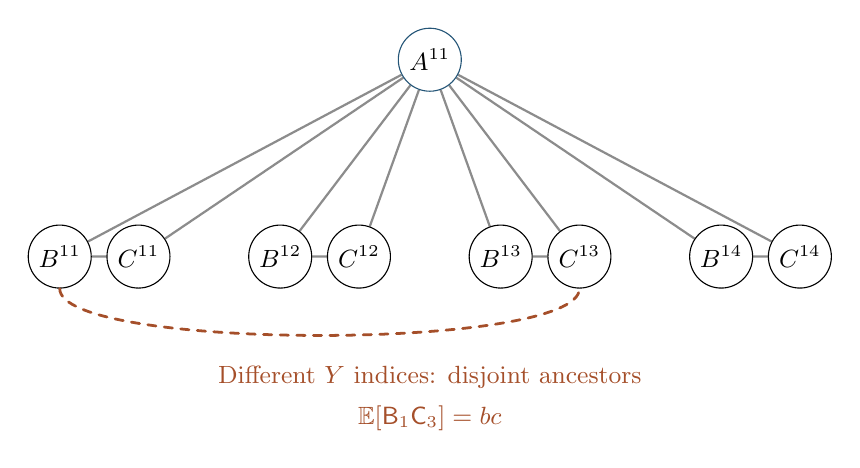
\begin{tikzpicture}[x=1cm,y=1cm]
\node[observer,draw=inkblue,minimum size=8mm] (a) at (4.7,2.5) {$A^{11}$};
\foreach \k/\x in {1/0,2/2.8,3/5.6,4/8.4}{
\node[observer,minimum size=8mm] (b\k) at (\x,0) {$B^{1\k}$};
\node[observer,minimum size=8mm] (c\k) at (\x+1,0) {$C^{1\k}$};
}
\begin{scope}[on background layer]
\foreach \k in {1,...,4}{\draw[network,black!45] (b\k)--(a)--(c\k) (b\k)--(c\k);}
\end{scope}
\draw[inkrust,dashed,line width=1pt] (b1.south) .. controls (0,-1.2) and (6.6,-1.2) .. (c3.south);
\node[font=\small,inkrust,align=center] at (4.7,-1.8) {Different $Y$ indices: disjoint ancestors\\[4pt]$\mathbb E[\mathsf B_1\mathsf C_3]=bc$};
\end{tikzpicture}
\caption{A fan with four copied triangles sharing $A^{11}$. Solid edges indicate shared ancestry within each triangle; the drawing is an incidence schematic. The cross pair $B^{1k},C^{1\ell}$ has disjoint ancestors for $k\ne\ell$ and can be placed in distinct diagonal rows. These cross moments yield both inequalities in Theorem~\ref{thm:fan}.}\label{fig:fan}
\end{figure}


\begin{proposition}[No uniformly divergent distance lower bound]\label{prop:Rp}
For $0<p<1$ let $R_p=(1-p)\delta_{111}+p\,\delta_{000}$. Then $R_p\notin\Ctri$, $R_p\to\delta_{111}$ as $p\downarrow0$, and $\tmin^H(R_p)=2$ for all three hierarchies and all $p$. Hence no inequality $\tmin^H(P)\ge c\,d_{\TV}(P,\Ctri)^{-\alpha}$ with $c,\alpha>0$ holds for all incompatible $P$; the growth in Proposition~\ref{prop:family} is a property of the direction of approach to the boundary.
\end{proposition}



\begin{proof}[Proof of Theorem~\ref{thm:fan}]
For $t=1$, the two inequalities reduce to $z\le a$ and $z^2\le az$, which hold since $0\le z\le a$. Now let $\Gamma$ be an order-$t$ feasible law for $P$, $t\ge2$, and consider the $2t+1$ copied observations $A^{11}$, $B^{1k}$, $C^{1k}$, $k\in[t]$: the fan (Figure~\ref{fig:fan}) of copied triangles $\Delta_{11k}=\{A^{11},B^{1k},C^{1k}\}$ sharing the vertex $A^{11}$. Define the indicators $\mathsf A=\one[A^{11}=0]$, $\mathsf B_k=\one[B^{1k}=0]$, $\mathsf C_k=\one[C^{1k}=0]$ and $T_k=\mathsf A\mathsf B_k\mathsf C_k$. Three identities follow from Definition~\ref{def:NW}: $\E\mathsf A=a$ and $\E T_k=z$, because a permutation of the $Y$-indices carries $\Delta_{11k}$ to the diagonal triangle $\Delta_{111}$, whose law is $P$; and for $k\ne\ell$,
\begin{equation}\label{eq:fan-cross}
\E[\mathsf B_k\mathsf C_\ell]=bc ,
\end{equation}
because the independent permutations $X_1\mapsto1$, $Z_1\mapsto2$, $Y_k\mapsto1$, $Y_\ell\mapsto2$ (extended arbitrarily to $[t]$) carry $B^{1k},C^{1\ell}$ to $B^{11},C^{22}$, which lie in the two diagonal triangles $\Delta_{111},\Delta_{222}$ whose joint law is $P\otimes P$ by the degree-two diagonal condition. The argument uses no product prescription beyond the diagonal law, and \eqref{eq:fan-cross} is not available for $k=\ell$.

\emph{First inequality.} For every deterministic assignment of the fan,
\begin{equation}\label{eq:fan-pointwise}
\sum_{k}\mathsf A\mathsf B_k\mathsf C_k\ \le\ \mathsf A+\frac12\sum_{k\ne\ell}\mathsf B_k\mathsf C_\ell .
\end{equation}
If $\mathsf A=0$ the left side vanishes. If $\mathsf A=1$, put $S=\sum_k\mathsf B_k\mathsf C_k$; then $\sum_k\mathsf B_k\ge S$ and $\sum_k\mathsf C_k\ge S$, so the right side is $1+\tfrac12\bigl[(\sum_k\mathsf B_k)(\sum_k\mathsf C_k)-S\bigr]\ge1+\tfrac12(S^2-S)$, and the right side minus the left side is at least $\tfrac12(S-1)(S-2)\ge0$ for every integer $S\ge0$. Taking expectations under $\Gamma$ and using the three identities gives $tz\le a+\binom t2bc$.

\emph{Second inequality.} Let $U=\sum_kT_k$. Since $U=\mathsf AU$, Cauchy--Schwarz gives $(\E U)^2\le\E\mathsf A\cdot\E U^2$, and $U^2=\sum_kT_k+\sum_{k\ne\ell}T_kT_\ell$ with $T_kT_\ell\le\mathsf B_k\mathsf C_\ell$. Hence $(tz)^2\le a[tz+t(t-1)bc]$, which rearranges to $t(z^2-abc)\le az-abc$.

\emph{Rejecting order.} If $z^2>abc$, the second inequality fails as soon as $t>(az-abc)/(z^2-abc)$; the fan can be rooted at whichever of $A,B,C$ has the smallest zero marginal, giving \eqref{eq:fan-order}. The ratio is at least $1$ since numerator minus denominator equals $z(\min\{a,b,c\}-z)\ge0$, so the bound is never below $2$, consistent with order one never rejecting. The smaller feasible sets of \eqref{eq:nested} reject no later.
\end{proof}

Inequality \eqref{eq:fan-pointwise} is a pointwise marginal-polytope certificate in the sense of \cite{WSF2019}, on a $1\times1\times t$ box of source copies; here it is available in closed form at every order.

\begin{proof}[Proof of Proposition~\ref{prop:Rp}]
$R_p$ has $a=b=c=z=p$, so $z^2=p^2>p^3=abc$ and Lemma~\ref{lem:finner} gives incompatibility. Order one is passed by every law. At order two the first fan inequality reads $2p\le p+p^2$, which fails for $p<1$; so $\tmin^H(R_p)=2$ for all three hierarchies, while $d_{\TV}(R_p,\Ctri)\le p\to0$.
\end{proof}

\subsection{Rejecting-order exponent along the family}\label{sec:exponent}


\begin{proposition}[One family with divergent rejecting order]\label{prop:family}
For $0<\eps<1/8$ let $P_\eps=Q\bigl(\eps,\,1-\tfrac12\eps^{2/3}\bigr)$, and write $\sigma=\tfrac12\eps^{2/3}$, $m=\eps+(1-\eps)\sigma$ for the common one-variable zero marginal and $z=\eps+(1-\eps)\sigma^3$ for $P_\eps(000)$. Then $P_\eps\notin\Ctri$, $P_\eps\to\delta_{111}\in\Ctri$ as $\eps\downarrow0$, and for $H\in\{\mathrm{exp},\mathrm{AI},\mathrm{NW}\}$ the first rejecting order $\tmin^H(P_\eps)=\min\{t:P_\eps\notin\mathcal I^H_t\}$ is finite and satisfies
\begin{gather*}
\Bigl\lfloor1+\tfrac12\eps^{-1/3}\Bigr\rfloor+1\ \le\ \tmin^H(P_\eps)\ \le\ \lfloor\tau_-(\eps)\rfloor+1\quad(\eps\le1/64),\\
\tau_-=\frac{z+m^2/2-\sqrt{(z+m^2/2)^2-2m^3}}{m^2},
\end{gather*}
so that
\[
\tfrac12\ \le\ \liminf_{\eps\downarrow0}\eps^{1/3}\tmin^H(P_\eps)\ \le\ \limsup_{\eps\downarrow0}\eps^{1/3}\tmin^H(P_\eps)\ \le\ 4-2\sqrt3\approx0.536 .
\]
In particular $\tmin^H(P_\eps)=\Theta(\eps^{-1/3})$ for each of the three hierarchies. \end{proposition}




\begin{proof}[Proof of Proposition~\ref{prop:family}]
Put $\sigma=\tfrac12\eps^{2/3}$, so $P_\eps=Q(\eps,1-\sigma)$, $m=\eps+(1-\eps)\sigma$ and $z=\eps+(1-\eps)\sigma^3$. \emph{Incompatibility:} $z\ge\eps$ and $m\le\eps+\sigma=\eps^{2/3}(\eps^{1/3}+\tfrac12)$, so $m^3<\eps^2\le z^2$ because $\eps^{1/3}<\tfrac12$ when $\eps<1/8$; Lemma~\ref{lem:finner} applies. \emph{Limit:} $\eps\to0$ and $1-\sigma\to1$, so $P_\eps\to\delta_{111}$, which is compatible. \emph{Lower bound:} if $t\le1+\tfrac12\eps^{-1/3}$ then $(t-1)\eps\le\sigma$, and Bernoulli's inequality gives $(1-\eps)^{t-1}\ge1-(t-1)\eps\ge1-\sigma$, so Theorem~\ref{thm:membership} applies with $r=1-\sigma$ and $P_\eps\in\Iexp_t$; hence every rejecting order exceeds $\lfloor1+\tfrac12\eps^{-1/3}\rfloor$. Finiteness is asymptotic completeness together with \eqref{eq:nested}.

\emph{Upper bound.} Write $v_t=tz-m-\binom t2m^2$; by the first fan inequality with $a=b=c=m$, positivity of $v_t$ rejects at order $t$. For $t=x\eps^{-1/3}+O(1)$ one has $tz=x\eps^{2/3}+O(\eps)$, $m=\tfrac12\eps^{2/3}+O(\eps)$ and $\binom t2m^2=\tfrac{x^2}8\eps^{2/3}+O(\eps)$, so
\[
v_t=\Bigl(x-\tfrac12-\tfrac{x^2}8\Bigr)\eps^{2/3}+O(\eps),
\]
whose leading coefficient is positive exactly for $4-2\sqrt3<x<4+2\sqrt3$. Fixing any $x$ slightly above $4-2\sqrt3$ gives rejection for all small $\eps$, which is the $\limsup$ bound. For the exact finite statement, $v_t$ is the quadratic $-\tfrac{m^2}2t^2+(z+\tfrac{m^2}2)t-m$ in $t$, with discriminant $D=(z+m^2/2)^2-2m^3$ and roots $\tau_\pm=(z+m^2/2\pm\sqrt D)/m^2$. For $\eps\le1/64$ one has $m\le\tfrac34\eps^{2/3}$ and $z\ge\eps$, so $D\ge\eps^2-2m^3\ge\eps^2(1-\tfrac{27}{32})=\tfrac5{32}\eps^2$ and $\tau_+-\tau_-=2\sqrt D/m^2\ge\tfrac{4\sqrt{10}}9\eps^{-1/3}>1$; since $v_1=z-m<0$ the integer $\lfloor\tau_-\rfloor+1$ lies strictly between the roots, where $v_t>0$. Hence $\tmin^{\mathrm{NW}}(P_\eps)\le\lfloor\tau_-\rfloor+1=(4-2\sqrt3)\eps^{-1/3}+O(1)$.

\end{proof}

\subsection{Distance to the compatible set}\label{sec:distance}

To express the rejecting-order exponent in terms of distance, we compute the leading distance from $P_\eps$ to $\Ctri$.

\begin{theorem}[Distance asymptotics]\label{thm:distance}
For $P_\eps=Q(\eps,1-\tfrac12\eps^{2/3})$, $0<\eps<1/8$,
\[
d_{\TV}(P_\eps,\Ctri)=\bigl(1-2^{-3/2}\bigr)\eps+O(\eps^{4/3}),\qquad
d_2(P_\eps,\Ctri)=\sqrt{8/7}\,\bigl(1-2^{-3/2}\bigr)\eps+O(\eps^{4/3}).
\]
\end{theorem}

\begin{corollary}[Direction-specific boundary complexity]\label{cor:geometry}
For $H\in\{\mathrm{NW},\mathrm{AI},\mathrm{exp}\}$,
\[
\tmin^H(P_\eps)=\Theta\bigl(d_{\TV}(P_\eps,\Ctri)^{-1/3}\bigr)=\Theta\bigl(d_2(P_\eps,\Ctri)^{-1/3}\bigr)\qquad(\eps\downarrow0).
\]
This is a statement about one direction of approach to the boundary; by Proposition~\ref{prop:Rp} no such lower bound holds uniformly over all incompatible laws.
\end{corollary}

\begin{proof}[Proof of Theorem~\ref{thm:distance}]
Put $\sigma=\tfrac12\eps^{2/3}$, $m=\eps+(1-\eps)\sigma$, $z=\eps+(1-\eps)\sigma^3$, $c_0=2^{-3/2}$ and $d_0=1-c_0$.

\emph{Lower bounds.} The product law $\Bern(1-\sigma)^{\otimes3}$ is compatible and within total variation $\eps$ of $P_\eps$. Compactness of $\Ctri$ gives a nearest law in either norm \cite{RGW2018}. A total-variation minimizer $Q$ therefore has distance $\delta=O(\eps)$. Since probabilities of events differ by at most $\delta$,
\[
Q(000)\ge z-\delta,\qquad Q_V(0)\le m+\delta\quad(V=A,B,C).
\]
Finner gives
\[
z-\delta\le(m+\delta)^{3/2}
 =c_0\eps+O(\eps^{4/3}),
\]
so $\delta\ge d_0\eps-O(\eps^{4/3})$.

A Euclidean minimizer $Q_2$ also satisfies $\|P_\eps-Q_2\|_2=O(\eps)$, by comparison with the product law. Cauchy--Schwarz bounds each one-variable marginal error by $2\|P_\eps-Q_2\|_2$, since each marginal sums four atoms. Hence Finner gives $Q_2(000)\le c_0\eps+O(\eps^{4/3})$. Set $D=P_\eps(000)-Q_2(000)$; then $D\ge d_0\eps-O(\eps^{4/3})>0$ for small $\eps$. The other seven coordinates of $Q_2-P_\eps$ sum to $D$, so
\[
\|Q_2-P_\eps\|_2^2\ge D^2+\frac{D^2}{7}.
\]
This proves the Euclidean lower bound.

\emph{A compatible approximation.} Set $h=d_0/7$ and $u=\sigma+(c_0+h)\eps$. Each source carries a base bit with success probability $\sqrt u$ and a flag with success probability $h\eps$, all six bits independent. A node outputs $0$ if both incident base bits equal $1$ or either incident flag equals $1$. These probabilities lie in $[0,1]$ for small $\eps$, and the resulting law $Q_\eps$ belongs to $\Ctri$.

Without flags, the atom probabilities are $u^{3/2}$ at $000$, $u-u^{3/2}$ at each one-zero atom, zero at each two-zero atom, and $1-3u+2u^{3/2}$ at $111$. A single flag forces the two nodes incident to its source to zero. Except on a base-output event of probability $O(u)$, it transfers mass from $111$ to the two-zero atom associated with that source. Multiple flags have probability $O(\eps^2)$. The errors from these exceptions are $O(\eps u+\eps^2)=O(\eps^{5/3})$.

Using $u^{3/2}=c_0\eps+O(\eps^{4/3})$ gives the following atom probabilities, with an $O(\eps^{4/3})$ remainder in each entry:
\begin{center}
\begin{tabular}{@{}lll@{}}
\toprule
Atom & $P_\eps$ & $Q_\eps$ \\
\midrule
$000$ & $\eps$ & $c_0\eps$ \\
Each of $011,101,110$ & $\sigma$ & $\sigma+h\eps$ \\
Each of $001,010,100$ & $0$ & $h\eps$ \\
$111$ & $1-3\sigma-\eps$ & $1-3\sigma-(c_0+6h)\eps$ \\
\bottomrule
\end{tabular}
\end{center}
Since $1-c_0=7h$, the deviation at $000$ is $-d_0\eps+O(\eps^{4/3})$ and at each of the other seven atoms it is $h\eps+O(\eps^{4/3})$. Its total variation is $d_0\eps+O(\eps^{4/3})$ and its Euclidean norm is $\sqrt{8/7}\,d_0\eps+O(\eps^{4/3})$, proving both upper bounds.
\end{proof}

Corollary~\ref{cor:geometry} follows from Theorem~\ref{thm:distance} and Proposition~\ref{prop:family}. The constant $1-2^{-3/2}$ is the fraction of the rare atom $P_\eps(000)\approx\eps$ that no compatible law can retain once its zero marginals are pinned near $\tfrac12\eps^{2/3}$, by the Finner inequality.


\section{Rejecting orders from distance and input size}\label{sec:input}

\subsection{Distance-promised rejecting orders}\label{sec:general}

Theorem~\ref{thm:main} says that the order needed cannot be fixed in advance for the scenario. For a single instance, Theorem~\ref{thm:convexorder} bounds it under a distance promise and Proposition~\ref{prop:bits} bounds it in the input size.

\begin{corollary}[Distance-promised rejecting order]\label{prop:promised}
Let $G$ be a correlation scenario with $K$ joint outcomes and let $\delta_2=d_2(P,\mathcal C_G)$ and $\delta=d_{\TV}(P,\mathcal C_G)$. If $P\in\INW_n(G)$ then
\begin{equation}\label{eq:nw-rate}
\delta_2^2\ \le\ \frac{1-\|P\|_2^2}{n},
\end{equation}
so for incompatible $P$
\[
\tmin^{\mathrm{NW}}(P)\ \le\ \Bigl\lfloor\frac{1-\|P\|_2^2}{\delta_2^2}\Bigr\rfloor+1\ \le\ \Bigl\lfloor\frac{K-1}{4\delta^2}\Bigr\rfloor+1 ;
\]
for the binary triangle, $\tmin^{\mathrm{NW}}(P)\le\lfloor7/(4\delta^2)\rfloor+1$.
\end{corollary}

\begin{proof}
The first inequality is \eqref{eq:convexl2}, since some $\omega$ attains at most the mean and $q_\omega$ is compatible. Feasibility at order $n$ then forces $n\le(1-\|P\|_2^2)/\delta_2^2$, and $\|P-Q\|_2^2\ge\|P-Q\|_1^2/K=4d_{\TV}(P,Q)^2/K$ with $\|P\|_2^2\ge1/K$ gives the second form. The triangle has $K=8$.
\end{proof}

The proof uses no convexity of $\mathcal C_G$: we extract one compatible law from the witness. A numerical lower bound on $\delta$ therefore suffices to choose a rejecting order; the result does not supply that lower bound from the input law.

\subsection{Rational input bit-length complexity}\label{sec:bits}

\begin{proposition}[Required order in the input size]\label{prop:bits}
Encode each of the eight rational atoms by its reduced numerator and positive denominator in ordinary binary, with delimiters of linear overhead. For a law $P$ on three bits, let $\ell(P)$ be its total bit length. For each $H\in\{\mathrm{NW},\mathrm{AI},\mathrm{exp}\}$,
\[
\max\bigl\{\tmin^H(P):\ \ell(P)\le B,\ P\notin\Ctri\bigr\}=2^{\Theta(B)} .
\]
\end{proposition}

\begin{proof}[Proof of Proposition~\ref{prop:bits}]
\emph{Lower bound.} With $k=2^j$, $\eps=k^{-3}$ and $\sigma=1/(2k^2)$, the eight atoms of $P_\eps$ are rationals with denominator $8k^9$ and numerators of $O(j)$ bits, so $\ell(P_\eps)=O(j)$, while Proposition~\ref{prop:family} gives $\tmin^H(P_\eps)>k/2=2^{j-1}$. Choosing $j$ proportional to $B$ gives $2^{\Omega(B)}$.

\emph{Upper bound.} By \cite{RGW2018}, $\Ctri$ is the image of a compact semialgebraic parameter space (six latent values per source and stochastic binary response tables) under a polynomial map, hence a closed semialgebraic subset of the simplex. The function $u(P)=d_2(P,\Ctri)^2$ is therefore semialgebraic, and its graph is described by a fixed quantifier-free formula $\Phi(P,u)$ in integer polynomials of fixed degrees, by real quantifier elimination \cite{BasuPollackRoy2006}. For a rational $P$ of bit length $B$, substituting $P$ and clearing denominators turns the atoms of $\Phi$ into univariate integer polynomials in $u$ of fixed degree and coefficient height $2^{O(B)}$. The set of $u$ satisfying $\Phi(P,u)$ is the single point $u(P)$; discard identically zero specialized polynomials, whose comparisons have constant truth values. If none of the remaining polynomials vanished at $u(P)$, their signs would persist on a neighbourhood and the formula would define an interval. Thus some nonzero specialized polynomial $f$ vanishes at $u(P)$. Remove any factor $u^r$ from $f$ to obtain $g(u)=a_0+\cdots+a_du^d$ with $a_0\ne0$, the same nonzero root, and coefficient height at most $H=2^{O(B)}$. For $0<u<1/(H+1)$,
\[
\Bigl|\sum_{i=1}^d a_i u^i\Bigr|\le H\sum_{i=1}^d u^i<\frac{Hu}{1-u}<1\le|a_0|,
\]
so $g(u)\ne0$. Hence $u(P)\ge2^{-O(B)}$ when $P$ is incompatible, and Corollary~\ref{prop:promised} gives $\tmin^{\mathrm{NW}}(P)\le(1-\|P\|_2^2)/u(P)+1=2^{O(B)}$; the two smaller feasible sets reject no later.
\end{proof}

With the binary triangle held fixed, a quantifier-free membership formula contains a bounded number of integer polynomials of bounded degree. Evaluating their signs at a rational input takes time polynomial in $B$. Quantifier elimination supplies such a formula in principle \cite{BasuPollackRoy2006}, although deriving and storing it may be impractical. Thus the exponential inflation-order bound coexists with a polynomial-time decision procedure for this fixed scenario. For an incompatible rational input, one can also compute the first rejecting order by enumerating exact rational feasibility problems.


\section{Open problems}\label{sec:open}

\begin{question}[Worst-case convergence exponent]\label{q:hausdorff}
For the square and the triangle, Corollary~\ref{cor:brackets} gives $\Omega(1/t)\le H_t^H\le O(t^{-1/2})$ for each hierarchy $H$. Which exponent in $[1/2,1]$ is sharp, and does it depend on the hierarchy?
\end{question}
For longer cycles Theorem~\ref{thm:cycle} gives $\Omega(m^{-2}t^{-2})$, and for the five-vertex path Theorem~\ref{thm:fivepath} gives $\Omega(t^{-2})$.

\begin{question}[Exact leading constant along the defect family]\label{q:constant}
Does $\eps^{1/3}\tmin^H(P_\eps)$ converge? If so, what is its limit, and do the three hierarchies share it?
\end{question}
The current bounds give the interval $[\tfrac12,4-2\sqrt3]$.

\begin{question}[Separation of the hierarchies]\label{q:separation}
Theorem~\ref{thm:orderconversion} shows that on the square the Navascués--Wolfe and ancestral-independence hierarchies differ by at most a factor $3/2$ in the order. Is the factor sharp, and does a bounded conversion hold on every pair-source scenario?
\end{question}
Proposition~\ref{prop:paritythresholds} gives finite-order separations. Whether $\IAI_t\subsetneq\INW_t$ holds at every order on any fixed scenario remains open.

\begin{question}[Beyond pair-source scenarios]\label{q:hypergraph}
Which scenarios with a source shared by three or more observed variables admit a finite characterizing order?
\end{question}
\begin{question}[Explicit rejecting orders beyond Finner]\label{q:effective}
Can one bound the rejecting order in directly evaluable quantities of an incompatible input law that satisfies every Finner inequality?
\end{question}
\begin{question}[Quantum and no-signalling analogues]\label{q:quantum}
For which quantum or no-signalling inflation hierarchies can one construct incompatible laws with an unbounded first rejecting order and determine its growth?
\end{question}

\section{Verification and availability}\label{sec:repro}

The sources, exact certificates and Lean development are available at \repo. The classification, witness constructions and asymptotic bounds have analytic proofs in the paper. The finite threshold claims in Proposition~\ref{prop:paritythresholds} additionally depend on rational primal and dual certificates, checked with integer and rational arithmetic and Sturm sequences. Figure~\ref{fig:thresholds} reads their endpoints directly. Appendix~\ref{app:certificates} describes the formats and finite coverage; the repository's \texttt{paper/review/VERIFICATION\_GUIDE.md} gives replay commands and checker details.

The Lean development proves the binary classification for finite latent alphabets, including the structural lemmas, double-star reconstruction, cycle and five-path obstructions, their distance lower bounds and local flips. It also proves the corrected triangle witness. The passage to arbitrary latent spaces uses the cardinality theorem of~\cite{RGW2018}, which is not formalized here. A separate triangle development proves the defect construction and nontermination for arbitrary latent probability spaces and measurable stochastic responses, the fan bounds, and the finite bounds on the defect family. It also proves the triangle norm estimates from Theorem~\ref{thm:convexorder}.

The general convex-order inequality, square corrected density and max-moment estimate, order conversion, count-moment and threshold results, distance asymptotics, bit-length theorem and supplementary inequalities are not formalized. Neither are the larger-observed-alphabet transfer or the limiting statements for the defect family. Declaration-level coverage appears in \texttt{README.md} and \texttt{formalization.yaml}; the axiom audit lists $112$ declarations.

The binary, finite-latent classification is registered as \texttt{PALOMAR-2026-09-14-000009}, version~1, at the \href{https://palomar-registry.org/entry.html?id=PALOMAR-2026-09-14-000009&version=1}{Palomar registry}. That registration concerns the stated classification theorem, not all results in this paper.


\clearpage
\appendix
\section{Structural details of inflation}\label{app:structure}

\subsection{The root-sink lemma}\label{app:rootsink}

We prove Lemma~\ref{lem:rootsink}, using the following description of active trails.

\begin{lemma}[Trail criterion]\label{lem:trail}
Let $X,Y,Z$ be disjoint sets of copied observations in the order-$t$ inflation of a pair-source scenario. Every trail between a member of $X$ and a member of $Y$ alternates copied observations and source copies, each source copy on it being a fork and each internal copied observation a collider. Such a trail is active given $Z$ if and only if all its internal copied observations lie in $Z$. Consequently $X\perp_dY\mid Z$ if and only if no trail from $X$ to $Y$ has all its internal copied observations in $Z$.
\end{lemma}

\begin{proof}
Every edge of the inflated graph joins a source copy to a copied observation, so the nodes of a trail alternate between the two kinds. A source copy has no parents, so both of its neighbours on the trail are its children and it is a fork; being a fork not in $Z$, since $Z$ consists of copied observations, it never blocks. An internal copied observation has no children, so both of its neighbours on the trail are its parents and it is a collider; a collider blocks unless it or one of its descendants lies in $Z$, and it has no descendants, so it blocks exactly when it is not in $Z$. A trail is active given $Z$ when no node on it blocks, which is the stated condition. The last sentence is the definition of $d$-separation.
\end{proof}

The shortest trails are the two-step ones, $x-S_e^{\,m}-y$, which have no internal observation and are therefore always active: two copied observations reading a common source copy are never $d$-separated.


\begin{proof}[Proof of Lemma~\ref{lem:rootsink}]
(i) If every component is injectable, then components with a common source copy would be joined, so distinct components are ancestrally independent and $W$ is their union. Conversely, let $W=W_1\cup\dots\cup W_m$ with the $W_r$ injectable and pairwise ancestrally independent. Every edge of the shared-parent graph joins two members reading a common source copy, hence two members of the same $W_r$. So each component lies in one $W_r$, and a subset of an injectable set is injectable.

(ii) Necessity: injectable sets are expressible by the first rule, and if $X$ and $Y$ are ancestrally independent then by Lemma~\ref{lem:trail} no trail from $X$ to $Y$ can avoid internal copied observations, and one with an internal copied observation is blocked by $\varnothing$; hence $X\perp_dY\mid\varnothing$ and the join rule with $Z=\varnothing$ prescribes $p(x)p(y)$. Iterating gives the products of Definition~\ref{def:gAI}.

Sufficiency: let $\Gamma$ satisfy the prescriptions of Definition~\ref{def:gAI}. We prove by induction on the generation of the expressible family that every generated set $W$ is an AI set and that the law prescribed for it agrees with the marginal $\Gamma_W$. By (i) and the AI prescriptions, the marginal of an AI set is the product of $P_{\pi(K)}$ over the components $K$ of its shared-parent graph.

For an injectable set the claim is the first AI prescription. For a marginal, the components of the shared-parent graph on a subset $W'\subseteq W$ are contained in those on $W$, hence injectable, so $W'$ is again an AI set, and the marginal of the prescription is the prescription of the marginal.

Consider the join rule with $X\perp_dY\mid Z$, where $X\cup Z$ and $Y\cup Z$ are already generated. Let $K$ be a connected component of the shared-parent graph on $X\cup Y\cup Z$ and suppose $K$ meets both $X$ and $Y$. Among all paths inside $K$ from a member of $X$ to a member of $Y$ choose one of minimal length. No internal vertex of it lies in $X$, since the subpath from that vertex to the $Y$-end would be shorter, and for the same reason none lies in $Y$; so every internal vertex lies in $Z$. Inserting between consecutive vertices a source copy they share turns this path into a trail from $X$ to $Y$ whose internal copied observations all lie in $Z$, which is active by Lemma~\ref{lem:trail} and contradicts $X\perp_dY\mid Z$. Hence every component of the shared-parent graph on $X\cup Y\cup Z$ lies in $X\cup Z$ or in $Y\cup Z$. Such a component is also a component of the shared-parent graph on the smaller set, since it is connected there and no member of the smaller set outside it is adjacent to it. As $X\cup Z$ and $Y\cup Z$ are AI sets, all these components are injectable, so $X\cup Y\cup Z$ is an AI set by (i).

It remains to check the prescribed law. Let $\mathcal K$ be the set of components of the shared-parent graph on $X\cup Y\cup Z$, split as $\mathcal X\sqcup\mathcal Y\sqcup\mathcal Z$ according to whether a component meets $X$, meets $Y$, or is contained in $Z$; by the previous paragraph no component meets both $X$ and $Y$, so this is a partition. Write $\alpha=\prod_{K\in\mathcal X}P_{\pi(K)}$, $\beta=\prod_{K\in\mathcal Y}P_{\pi(K)}$ and $\mu=\prod_{K\in\mathcal Z}P_{\pi(K)}$, each evaluated at the coordinates of its component. The components of the shared-parent graph on $X\cup Z$ are the members of $\mathcal X\cup\mathcal Z$ together with the components of $K\cap Z$ for $K\in\mathcal Y$; write $\nu_{\mathcal Y}$ for the product of $P_{\pi(C)}$ over the latter, and $\nu_{\mathcal X}$ for the analogous product coming from $\mathcal X$ inside $Y\cup Z$. Then
\[
\Gamma_{X\cup Z}=\alpha\,\mu\,\nu_{\mathcal Y},\qquad
\Gamma_{Y\cup Z}=\beta\,\mu\,\nu_{\mathcal X},\qquad
\Gamma_{Z}=\mu\,\nu_{\mathcal X}\,\nu_{\mathcal Y},
\]
the last because the components of the shared-parent graph on $Z$ are those of $K\cap Z$ for $K\in\mathcal X\cup\mathcal Y$ together with $\mathcal Z$. At a point where $\Gamma_Z>0$ the factors $\mu$, $\nu_{\mathcal X}$ and $\nu_{\mathcal Y}$ are positive and cancel,
\[
\frac{\Gamma_{X\cup Z}\,\Gamma_{Y\cup Z}}{\Gamma_{Z}}=\alpha\,\beta\,\mu=\Gamma_{X\cup Y\cup Z},
\]
which is the prescribed value. Where $\Gamma_Z=0$ the rule prescribes $0$, and $\Gamma_{X\cup Y\cup Z}\le\Gamma_Z=0$ there, so the two agree on zero fibres as well. This completes the induction.
\end{proof}

\subsection{Induced-subgraph transport}\label{app:transport}

\begin{proof}[Proof of Lemma~\ref{lem:transport}]
(i) Take a $G$-model for $Q$ and keep the observations at $V(H)$. Since $H$ is induced, every edge of $G$ with both endpoints in $V(H)$ is an edge of $H$. An edge of $G$ with exactly one endpoint $v$ in $V(H)$ has its source read, among the retained observations, only by $v$; append that source to the source of one edge of $H$ at $v$, which exists because $v$ is not isolated in $H$, and let the other endpoint of that edge ignore the appended component. The result is an $H$-model with the same observed law on $V(H)$.

(ii) Let $\Gamma^H$ be a witness for $P_H$ at order $t$ and write $E_H(v)$ for the set of edges of $H$ at $v$. Define a table $\Gamma$ for $G$ as follows: draw the copied observations $(O_v^{\,j})_{v\in V(H),\,j\in[t]^{E_H(v)}}$ from $\Gamma^H$, draw independent fair bits $\xi_w^{\,k}$ for $w\notin V(H)$ and $k\in[t]^{E(w)}$, and set
\[
O_v^{\,i}:=O_v^{\,i|_{E_H(v)}}\ (v\in V(H)),\qquad O_w^{\,k}:=\xi_w^{\,k}\ (w\notin V(H)),
\]
so that a copied observation at an $H$-vertex ignores the indices of the edges leaving $H$.

Symmetry: a permutation of the copy indices of an edge of $H$ acts on the first family as the corresponding element of the symmetry group of the $H$-inflation and fixes the fair bits; a permutation of the copy indices of any other edge leaves every $O_v^{\,i}$ with $v\in V(H)$ unchanged and permutes the fair bits among themselves, which preserves their law. Diagonal law: row $r$ of the $G$-inflation restricted to $V(H)$ is row $r$ of the $H$-inflation, and the outside entries of the $t$ rows are $t|V\setminus V(H)|$ distinct fair bits, so the diagonal law is $P_H^{\otimes t}\otimes\Bern(1/2)^{\otimes t(V\setminus V(H))}=P^{\otimes t}$.

Injectable prescriptions: let $S$ be injectable in the $G$-inflation with $W=\pi(S)$. Its members at $H$-vertices, with the outside indices dropped, form an injectable set of the $H$-inflation, because index erasure is still injective and the indices on the edges of $H$ still agree; so their joint law under $\Gamma$ is $(P_H)_{W\cap V(H)}$. Its members at outside vertices are distinct fair bits, independent of everything else, and $P_{W}=(P_H)_{W\cap V(H)}\otimes\Bern(1/2)^{\otimes(W\setminus V(H))}$, as required. Ancestrally independent families: source copies of edges of $H$ are source copies in $G$ as well, so ancestrally independent injectable sets of the $G$-inflation have ancestrally independent $H$-parts, whose laws multiply under $\Gamma^H$, while the fair bits are independent of them and of each other. Hence $\Gamma$ satisfies the conditions of Definition~\ref{def:gAI} whenever $\Gamma^H$ does. The expressible case follows from the AI case by Lemma~\ref{lem:rootsink}, applied in $H$ and in $G$.

(iii) For $Q\in\Cscen{G}$, part (i) gives $Q_{V(H)}\in\Cscen{H}$, and marginalization does not increase total variation, so $d_{\TV}(P,Q)\ge d_{\TV}(P_{V(H)},Q_{V(H)})=d_{\TV}(P_H,Q_{V(H)})\ge d_{\TV}(P_H,\Cscen{H})$. Taking the infimum over $Q$ gives the claim.
\end{proof}

\subsection{Injectable sets of the triangle}\label{app:injectable}

We justify the description of injectable sets used in Definition~\ref{def:AI}. In the order-$t$ inflated triangle, a set $S$ of copied observations is injectable when the map that erases copy indices is injective on $S$ and, for any two members of $S$ that are copies of variables sharing a source in the triangle, the copy index of that source agrees \cite[Definition~4]{WSF2019}. Injectivity allows at most one copy of each of $A$, $B$, $C$. If $S$ contains $A^{ij}$ and $B^{i'k}$ then $i=i'$; if it contains $A^{ij}$ and $C^{j'k}$ then $j=j'$; if it contains $B^{ik}$ and $C^{jk'}$ then $k=k'$. Hence $S\subseteq\Delta_{ijk}$ for suitable $(i,j,k)$, any missing index being chosen freely. Conversely every subset of a copied triangle is injectable. This proves the characterization for all $t$.

The degree-$t$ diagonal condition (ii) of Definition~\ref{def:NW} also implies the lower-degree conditions of \cite{NW2020}: the law of any $g\le t$ diagonal triangles is a marginal of $P^{\otimes t}$, hence $P^{\otimes g}$, and by symmetry the same holds for any $g$ copied triangles with pairwise distinct indices in all three families.

\section{Order conversion and finite thresholds}\label{app:quantitative}

\subsection{Proof of square order conversion}\label{app:conversion}

\begin{proof}[Proof of Theorem~\ref{thm:orderconversion}]
The right inclusion is Proposition~\ref{prop:gsound} and the equality is Lemma~\ref{lem:rootsink}. For the left inclusion let $\Gamma$ be an order-$n$ Navascu\'es--Wolfe witness for $P$ with $n=\lfloor3t/2\rfloor$ and let $\Gamma'$ be its restriction to the copy indices $1,\dots,t$ of each source. Restriction preserves symmetry and the diagonal law of degree $t$, so $\Gamma'\in\INW_t$; we check the AI prescriptions.

Fix an AI set of $\Gamma'$ and decompose it into the connected components of its shared-parent graph, which are injectable and pairwise ancestrally independent. A component's ancestry uses two, three or four source types; the two-type components are single copied observations and correspond to edges of the four-cycle $X-Y-Z-W-X$ of source types. Any two subsets of a four-element set of sizes at least three, or of sizes three and two, intersect, so a component using at least three source types conflicts with every other component and needs a diagonal row of its own. Let $b$ be the number of these.

The remaining components form a multigraph on the source-type four-cycle, with multiplicities $n_A,n_B,n_C,n_D$ on the edges $A,B,C,D$. Opposite edges are disjoint, so the colours $\max(n_A,n_C)$ for the pair $\{A,C\}$ and $\max(n_B,n_D)$ for the pair $\{B,D\}$ suffice, and their sum equals the maximum source-type degree $\Delta$: if $n_A\ge n_C$ and $n_B\ge n_D$ the sum is $n_A+n_B=\deg X$, and $\deg X$ dominates the other three degrees. So $b+\Delta$ rows suffice.

Choose a source type of residual degree $\Delta$, say $X$, together with its two neighbours $Y$ and $W$ on the cycle. A component using at least three source types omits at most one, so it uses at least two of $X,Y,W$; each of the $\Delta$ two-type components incident to $X$ uses exactly two of them. The components have pairwise disjoint copied ancestries, and the three families $X,Y,W$ supply $3t$ copies in $\Gamma'$, so $2b+2\Delta\le3t$ and therefore $b+\Delta\le\lfloor3t/2\rfloor=n$.

Assign each component to the diagonal row of its colour. Components sharing a row use disjoint source types, and distinct components use distinct copies within each family, so independent permutations of the copy indices of the four sources place all components on their assigned rows simultaneously. Under $\Gamma$ the rows are independent with law $P$. Within one row the components have disjoint original source types, so Lemma~\ref{lem:sourcedisjoint}, available because $n\ge2$, makes $P$ factor across them. Hence the joint law of the placed components is the product of their $P$-marginals. Undoing the permutations, the AI set of $\Gamma'$ has exactly the prescribed product.
\end{proof}

The factor $3/2$ is the cost of placing all components on diagonal rows at once; ancestrally disjoint collections of $\lfloor3t/2\rfloor$ injectable components whose source-type conflict graph is complete show that this method cannot do better.

\subsection{Count-moment reductions}\label{app:countmoment}

The reductions below replace feasibility for a parity-perfect target by a linear program on the counts of negative auxiliary signs.

\begin{lemma}[Count-moment reduction]\label{lem:countmoment}
Let $0\le q\le3-2\sqrt2$ and $t\ge1$. Then $P_q\in\IAI_t(\square)$ if and only if there are $w_a\ge0$, $a=(a_X,a_Y,a_Z,a_W)\in\{0,\dots,t\}^4$, with $\sum_aw_a=1$ and
\begin{equation}\label{eq:countmoment}
\sum_aw_a\prod_{g}K^{(t)}_{k_g}(a_g)=(-q)^{S/2},\qquad S=\sum_gk_g,
\end{equation}
for exactly those degree tuples $k\in\{0,\dots,t\}^4$ with $S$ even and $2\max_gk_g\le S$, where
\[
K^{(t)}_k(a)=\binom tk^{-1}\sum_j(-1)^j\binom aj\binom{t-a}{k-j}
\]
is the normalized Krawtchouk polynomial.
\end{lemma}

\begin{proof}
Every copied square is injectable, so under any witness it has law $P_q$ and hence parity $+1$ almost surely. Parity forcing across the copy indices then gives sign potentials: from $A^{il}B^{ij}C^{jk}D^{kl}=1$ for all indices, the product $B^{ij}C^{jk}$ depends only on $(i,k)$, so writing $M^{ik}$ for it and $x_i=M^{i1}$, $y_j=C^{j1}$ gives $B^{ij}=x_iy_j$ and, by the same argument on the other pairs, every supported array is of the form $A^{il}=x_iw_l$, $B^{ij}=x_iy_j$, $C^{jk}=y_jz_k$, $D^{kl}=z_kw_l$. The potential is unique up to the simultaneous flip of all four families, so averaging over the two gauges and over independent permutations of the copy indices reduces a witness to a distribution on the four counts $a_g$ of negative signs. Under that symmetrization the average of a character with $k_g$ distinct indices in family $g$ is $\prod_gK^{(t)}_{k_g}(a_g)$, by the definition of the Krawtchouk polynomial as the mean of a $k$-element sign product drawn without replacement.

It remains to characterize the prescribed degrees. Within one injectable block the boundary has even size and uses each source family at most once. Thus each family contributes at most half the size of that boundary. Boundaries of ancestrally independent blocks are disjoint, so their total degrees satisfy $S$ even and $2\max_gk_g\le S$.

Conversely, regard $k_g$ as the number of terminals in source family $g$, arranged around the source cycle $X-Y-Z-W-X$. A path between two distinct source families gives an injectable block whose boundary consists of its endpoints. We construct paths using at most $t$ copies of each family, with distinct copies assigned to distinct paths. Write $(a,b,c,d)=(k_X,k_Y,k_Z,k_W)$ and, after a cyclic relabelling if necessary, assume $a+c\ge b+d$. Put $r=(a+c-b-d)/2$. The balance condition gives $0\le r\le\min(a,c)$. Pair $r$ terminals of $X$ with $r$ terminals of $Z$. The remaining $X,Z$ terminals number $b+d$ and can be paired with the $Y,W$ terminals along adjacent edges, since each of $X,Z$ is adjacent to each of $Y,W$. Route each of the $r$ opposite pairs through either $Y$ or $W$. There are $2t-b-d$ unused copies in those two families, and
\[
r=\frac{a+c-b-d}{2}\le t-\frac{b+d}{2}\le2t-b-d.
\]
These copies suffice for the internal vertices. Assigning distinct copies at every terminal and internal vertex makes the resulting injectable blocks ancestrally independent. Their joint character has the required degree tuple and prescribed value $(-q)^{S/2}$. Thus the listed equations are necessary and sufficient.
\end{proof}

\begin{lemma}[The Navascu\'es--Wolfe form]\label{lem:countmomentNW}
Under the hypotheses of Lemma~\ref{lem:countmoment}, $P_q\in\INW_t(\square)$ if and only if \eqref{eq:countmoment} holds for exactly the degree tuples in
\[
D_{\mathrm{NW}}(t)=\{b_1+\dots+b_t:\ b_r\in\{0,1\}^4\text{ of even weight}\}\subseteq D_{\mathrm{AI}}(t),
\]
where $D_{\mathrm{AI}}(t)$ is the degree set of Lemma~\ref{lem:countmoment}. The same reductions hold for the triangle family $\Pi(-q,-q,-q)$ with three families of signs and the potentials $A^{ij}=x_iz_j$, $B^{ik}=x_iy_k$, $C^{jk}=z_jy_k$.
\end{lemma}

\begin{proof}
Every copied square is carried to the first diagonal row by independent copy-index permutations, so under a symmetric witness with diagonal law $P_q^{\otimes t}$ it has law $P_q$ and parity $+1$; the potential representation and the symmetrization then proceed as in Lemma~\ref{lem:countmoment}. The diagonal law prescribes exactly the characters $\prod_r\prod_{v\in F_r}O_v^{(r)}$ with one vertex set $F_r$ per diagonal row; in potential form row $r$ contributes the indicator of $\partial F_r$ to the degree tuple, and the boundaries of vertex sets of a cycle are exactly its even-weight edge sets. Conversely a distribution on counts with the prescribed moments yields a symmetric witness with the diagonal law by the construction in the proof of Lemma~\ref{lem:countmoment}. For the triangle, balanced degrees $(a,b,c)$ are realized by $(a+b-c)/2$, $(b+c-a)/2$ and $(c+a-b)/2$ single-observation blocks between the respective source pairs; these counts are nonnegative integers and use exactly the prescribed number of copies. Also, $A^{ij}B^{ik}C^{jk}=1$ at $j=1$ gives $B^{ik}=A^{i1}C^{1k}$, so $x_i=A^{i1}$ and $y_k=C^{1k}$ serve as potentials for $B$, and $z_j=A^{1j}x_1$ completes the representation, unique up to a global flip.
\end{proof}

\begin{lemma}[Monotonicity along the parity direction]\label{lem:paritymonotone}
Let $H\in\{\mathrm{NW},\mathrm{AI},\mathrm{exp}\}$, $G\in\{\triangle,\square\}$, and $0\le q'\le q$ in the range where the parity target is a law. If the parity target with parameter $q$ lies in $I^H_t(G)$, so does the one with parameter $q'$.
\end{lemma}

\begin{proof}
If $q=0$, then $q'=0$ and there is nothing to prove. For $q>0$, Lemmas~\ref{lem:countmoment} and~\ref{lem:countmomentNW} let us take a witness to be a law on sign potentials. Multiply every potential sign by an independent $\pm1$ variable of mean $\rho=\sqrt{q'/q}$. A character whose boundary has $S$ elements is multiplied by $\rho^S$, so its value $(-q)^{S/2}$ becomes $(-q')^{S/2}$, while symmetry and the block structure of every prescription are unchanged. Lemma~\ref{lem:rootsink} covers the recursively expressible test.
\end{proof}


\subsection{Certified threshold brackets}\label{app:thresholds}

\begin{table}
\centering
\small
\renewcommand{\arraystretch}{1.15}
\begin{tabular}{r@{\quad}ll@{\qquad}ll}
\toprule
& \multicolumn{2}{c}{square} & \multicolumn{2}{c}{triangle}\\
\cmidrule(lr){2-3}\cmidrule(lr){4-5}
$t$ & $q^{\mathrm{AI}}_t$ & $q^{\mathrm{NW}}_t$ & $q^{\mathrm{AI}}_t$ & $q^{\mathrm{NW}}_t$\\
\midrule
1 & $3-2\sqrt2$ & $3-2\sqrt2$ & $1/3$ & $1/3$\\
2 & $0.1324743290$ & $\ge0.1715628752$ & $0.2679491900$ & $1/3$\\
3 & $0.0950228950$ & $0.0950228950$ & $0.1999999980$ & $0.1999999980$\\
4 & $0.0835279580$ & $0.0950228950$ & $0.1730047060$ & $0.1999999980$\\
5 & $0.0657380020$ & $0.0657380020$ & $0.1428571400$ & $0.1428571400$\\
6 & $0.0603176600$ & $0.0645356170$ & $0.1283741760$ & $0.1381856900$\\
7 & $0.0502565110$ & $0.0502565110$ & $0.1092774840$ & $0.1092774840$\\
8 & $0.0470271490$ & $0.0494541280$ & $0.1011416960$ & $0.1070388380$\\
9 & $0.0406784540$ & $0.0406784540$ & $0.0888129680$ & $0.0888129680$\\
10 & $0.0384981990$ & $0.0400943600$ & $0.0833179940$ & $0.0870307060$\\
\bottomrule
\end{tabular}
\caption{Certified brackets for the parity thresholds. A decimal entry $x$ means $x\le q^H_t\le x+4\cdot10^{-9}$; the exact entries at order one and triangle NW order two follow from the endpoint laws and Proposition~\ref{prop:lowextraction}; the entry $\ge0.1715628752$ is a lower bound only, the family ending at $3-2\sqrt2\approx0.1715728753$.}\label{tab:thresholds}
\end{table}

\begin{proof}[Proof of Proposition~\ref{prop:paritythresholds}]
For each order and hierarchy, the artifact contains a nonnegative rational count distribution at the lower endpoint and rational dual functionals whose expectation polynomials are positive on intervals covering $[q_{\mathrm{hi}},q_{\mathrm{cap}}]$. The checker verifies every prescribed moment, dual nonpositivity on all count configurations, and the interval signs by Sturm sequences. Here $q_{\mathrm{cap}}=1/3$ for the triangle and $q_{\mathrm{cap}}=1715728752/10^{10}<3-2\sqrt2$ for the square. For each two-sided bracket, monotonicity (Lemma~\ref{lem:paritymonotone}) extends rejection at $q_{\mathrm{cap}}$ to the remainder of the physical range, and extends the primal witness down to zero. The verification guide linked in Section~\ref{sec:repro} gives the files and commands.

Order one accepts every target law. Proposition~\ref{prop:lowextraction} gives the triangle NW order-two endpoint. The strict comparisons follow by comparing rational endpoints. On the square, the points $3/20$ and $1/10$ lie in the respective gaps; Theorem~\ref{thm:orderconversion} supplies the inclusion $\INW_3\subseteq\IAI_2$.
\end{proof}

Some dual expectation polynomials have simple roots, including $2-\sqrt3$, $1/5$ and $1/7$ in the triangle cases. A root yields an upper obstruction; an exact threshold identity would also require a primal witness at that root.

\section{Certificate formats and coverage}\label{app:certificates}

The files described here are under \texttt{artifact/certificates/} in the repository \repo, with the checkers under \texttt{artifact/verifiers/} and the manifest of SHA-256 identities at \texttt{artifact/MANIFEST.json}.

\paragraph{Structural certificate at order $t$.}
A JSON object with the root law (kind, $\eps_t=1/(2t^3)$ and $1-\eps_t$ as exact fractions), the value $r_t$, the list of $t^3$ roots $D_{ijk}$, for each of the $3t^2$ outputs the list of roots on its line, the eight target atoms of $P_t$ as exact fractions, and the claimed counts of diagonal equations ($8^t$) and symmetry generators ($3(t-1)$). The checker recomputes every claimed quantity from the definitions and compares exactly. The checker computes the copied-triangle marginals by enumerating the $2^{3t-2}$ assignments of the roots on the three lines through a cell, which makes $t=3$ (with $2^7$ assignments per triangle and $8^3=512$ diagonal equations) immediate.

\paragraph{Full order-two table.}
A JSON object listing the $12$ observation names in a fixed order, the denominator $2^{32}=(2t^3)^{t^3}$ at $t=2$, and the nonzero numerators $\Gamma_2(w)$ of \eqref{eq:table} for $166$ assignments $w\in\{0,1\}^{12}$; unlisted assignments have numerator $0$. The checker verifies $\sum_w\Gamma_2(w)=1$, nonnegativity, $\Gamma_2(w)=\Gamma_2(\pi w)$ for the three adjacent transpositions $\pi$ and all $4096$ assignments, and the $64$ equations $\sum_{w:\,w_{\mathrm{diag}}=(x,y)}\Gamma_2(w)=P_2(x)P_2(y)$ for the diagonal coordinates $(A^{11},B^{11},C^{11},A^{22},B^{22},C^{22})$.

\paragraph{Negative control.}
The same object with the numerators of the all-one and all-zero assignments changed by $-1$ and $+1$. Normalization and nonnegativity hold; the diagonal equation at $(000,000)$ fails. The checker is required to reject it.

\paragraph{Promised-rejection calibration.}
An exact Farkas certificate showing that the rational law $\tfrac12(\delta_{000}+\delta_{111})$ is infeasible at order two with margin $1/2$, which checks rejection of $R_{1/2}$ from Proposition~\ref{prop:Rp}. This finite check does not certify the general convergence constants.

\paragraph{Fan certificates.}
A JSON list of records, one per $k$ in the list $4$, $5$, $6$, $8$, $10$, $16$, $32$, $64$, $128$, $256$, $512$, $1024$, $4096$, $65536$, with $\eps=k^{-3}$, $\sigma=1/(2k^2)$, the eight exact atoms of $P_\eps$, the values $m$, $z$ and the Finner gap $z^2-m^3$, the passing order $\lfloor1+k/2\rfloor$ with the exact Bernoulli certificate $(t-1)\eps\le\sigma$, the first order at which $v_t=tz-m-\binom t2m^2$ is positive together with the exact rational value of $v_t$ there, and the first order at which the second-moment inequality fails. An all-order certificate records the identity $1+\tfrac12S(S-1)-S=\tfrac12(S-1)(S-2)$ and its nonnegativity on integers by cases, so that \eqref{eq:fan-pointwise} needs no order-by-order enumeration; the checker nevertheless enumerates all assignments of the fan for small $t$ and all count orbits for larger $t$, and verifies that the index permutations used in \eqref{eq:fan-cross} extend to permutations of $[t]$. Negative controls perturb the atoms, the parameters and the claimed orders and must be rejected.

\subsection{Finite coverage}

\begin{table}[htbp]
\centering\small
\renewcommand{\arraystretch}{1.12}
\begin{tabular}{@{}>{\raggedright\arraybackslash}p{.21\linewidth}>{\raggedright\arraybackslash}p{.23\linewidth}>{\raggedright\arraybackslash}p{.48\linewidth}@{}}
\toprule
Certificate set & Range & Checked properties\\
\midrule
Defect cube & $t=1,2,3$ & Root probabilities, line supports, symmetry, copied-triangle marginals, diagonal products and Finner gaps.\\[3pt]
Full defect table & $t=2$ & All $4096$ assignments; $166$ nonzero entries; $12{,}288$ symmetry equations and $64$ diagonal equations.\\[3pt]
Fan inequalities & Fourteen rational targets & Passing bounds, fan and second-moment rejection bounds, the pointwise count identity, index embeddings and negative controls.\\[3pt]
Classification witnesses & Cycles $C_3,C_4,C_5$ and path: $t\le2$; corrected triangle: $t\le3$ & Auxiliary density, nonnegative observed law, symmetry, prescribed marginals and ancestral products, target separation and local flips where supplied.\\[3pt]
Parity thresholds & Triangle and square, both tests, $1\le t\le10$ & Primal moments, dual signs on every count configuration, interval positivity; brute-force AI degree enumeration for $t\le3$ and explicit realizations through $t=10$.\\
\bottomrule
\end{tabular}
\caption{Finite certificate coverage. Positivity of an auxiliary density does not imply full support of its observed pushforward. The unflipped cycle witnesses have parity constraints.}\label{tab:verification}
\end{table}

The fan bounds determine the first rejecting orders of $P_\eps$ exactly at $\eps=k^{-3}$ for $k=4,6,8,10,16$: they are $4,5,6,7,10$. At $k=32,128,1024,65536$, the passing construction gives lower bounds $18,66,514,32770$, while the fan gives upper bounds $19,70,551,35122$.

\providecommand{\Csq}{\mathcal C_{\square}}
\providecommand{\Cpar}{\mathcal C_{\mathrm{par}}}
\providecommand{\Par}[3]{\Pi(#1,#2,#3)}
\section{Supplementary inequalities and extraction results}\label{app:supporting}

We give three complements to the main proofs: a stronger fan inequality and its square specialization, bounds for independent-cell constructions, and two limitations of extraction from a supported table. Throughout, total variation is half the $\ell^1$ distance.

\subsection{A fan inequality retaining pair marginals}

\begin{proposition}[Pair-retaining fan inequality]\label{prop:pairfan}
Let $n\ge2$ and let $P$ be a law on three bits with $a=P_A(0)$, $b=P_B(0)$, $c=P_C(0)$, $d=P_{AB}(00)$, $g=P_{AC}(00)$ and $z=P(000)$. If $P\in\INW_n$ then
\begin{equation}\label{eq:pairfan}
d+g+(n-2)z\ \le\ a+\binom n2bc .
\end{equation}
\end{proposition}

\begin{proof}
For bits $b_1,\dots,b_n,c_1,\dots,c_n$ put $U=\sum_kb_k$, $V=\sum_kc_k$, $W=\sum_kb_kc_k$. The pointwise inequality is
\begin{equation}\label{eq:pairfan-pointwise}
UV-W\ \ge\ \frac2n\bigl((n-2)W+U+V-n\bigr).
\end{equation}
To see it, multiply by $n$ and collect terms on one side as $R=nUV-(3n-4)W-2U-2V+2n$. Since $W\le\min(U,V)$ and its coefficient is negative, it suffices to treat $W=\min(U,V)$; assume $U\le V$, so $R$ becomes $nUV-(3n-2)U-2V+2n$. For $U=0$ this is $2(n-V)\ge0$; for $U=1$ it is $(n-2)(V-1)\ge0$; for $U\ge2$ it increases in $V$, so its minimum is at $V=U$, where it equals $n(U-1)(U-2)\ge0$.

Now take the fan of the proof of Theorem~\ref{thm:fan}: $\mathsf A=\one[A^{11}=0]$, $\mathsf B_k=\one[B^{1k}=0]$, $\mathsf C_k=\one[C^{1k}=0]$, and set $b_k=\mathsf B_k$, $c_k=\mathsf C_k$ in \eqref{eq:pairfan-pointwise}. Definition~\ref{def:NW} gives $\E\mathsf A=a$, $\E[\mathsf A\mathsf B_k]=d$, $\E[\mathsf A\mathsf C_k]=g$ and $\E[\mathsf A\mathsf B_k\mathsf C_k]=z$, since a permutation of the $Y$-indices carries each of these sets into the diagonal triangle $\Delta_{111}$, and $\E[\mathsf B_k\mathsf C_\ell]=bc$ for $k\ne\ell$ by \eqref{eq:fan-cross}. Hence $\E(UV-W)=n(n-1)bc$. Multiplying \eqref{eq:pairfan-pointwise} by $\mathsf A$ and using $UV-W\ge0$ gives
\[
n(n-1)bc\ \ge\ \frac2n\bigl(n(n-2)z+nd+ng-na\bigr),
\]
which rearranges to \eqref{eq:pairfan}.
\end{proof}

Since $d\ge z$ and $g\ge z$, \eqref{eq:pairfan} implies the first inequality of \eqref{eq:fan}. We apply it to the square through a conditioning that costs no order.

\begin{lemma}[Same-order transfer]\label{lem:sqtri}
Let $n\ge2$ and $P\in\INW_n(\square)$. Then $P_{ABC\mid D=1}\in\INW_n(\triangle)$ whenever $P_D(1)>0$, and in every case
\begin{equation}\label{eq:sqtri}
P_{ABD}(001)+P_{ACD}(001)+(n-2)P(0001)\ \le\ P_{AD}(01)+\binom n2P_B(0)P_{CD}(01).
\end{equation}
\end{lemma}

\begin{proof}
Condition an order-$n$ square witness on $D^{11}=\dots=D^{nn}=1$, an event of probability $P_D(1)^n>0$, and retain the complete $A,B,C$ arrays. Independent permutations of the $X$- and $Y$-indices, together with the simultaneous permutation of the $Z$- and $W$-indices, realize the three source symmetries of the triangle, and the conditional diagonal law is $(P_{ABC\mid D=1})^{\otimes n}$. Applying \eqref{eq:pairfan} to the conditional law, using the independence of $B$ and $D$ forced at order $n\ge2$, and clearing the positive denominator gives \eqref{eq:sqtri}. If $P_D(1)=0$ every term of \eqref{eq:sqtri} containing $D=1$ vanishes and the inequality is trivial.
\end{proof}


\subsection{Independent-cell constructions}

Consider independent cell roots and symmetric line responses. Let $U_{ijk}$, $(i,j,k)\in[n]^3$, be independent with a common law $\mu$ on a finite alphabet, let each observed type $V\in\{A,B,C\}$ carry a permutation-invariant kernel $g_V$ giving its probability of output one from the $n$ roots on its line, and let the responses be independently randomized across copied observations. The resulting table is a full order-$n$ witness, and with the profiles $f_V(s)=\E[g_V(s,U_2,\dots,U_n)]$ and $m_V=\sum_s\mu_sf_V(s)$ the target is $\sum_s\mu_s\bigotimes_V\Bern(f_V(s))$. Write $\mathcal L_n^{(\kappa)}$ for the laws obtained this way from a root alphabet of size $\kappa$.

\begin{lemma}[Profile variance]\label{lem:cellvar}
For every admissible line kernel, $\operatorname{Var}_\mu(f_V)\le m_V(1-m_V)/n$.
\end{lemma}

\begin{proof}
Write $f=f_V$, $m=m_V$, $h=f-m$, $v=\E h(U)^2$ and $T=\sum_{i=1}^nh(U_i)$, and let $g=g_V(U_1,\dots,U_n)$. Independence gives $\E T^2=nv$, and symmetry of the kernel gives $\E[(g-m)T]=n\E[h(U_1)(g-m)]=nv$. Cauchy--Schwarz then give $(nv)^2\le\operatorname{Var}(g)\,nv$. For $v>0$ divide by $nv$ and use $0\le g\le1$ to get $nv\le\operatorname{Var}(g)\le m(1-m)$; the case $v=0$ is immediate.
\end{proof}

\begin{proposition}[Independent-cell ceilings]\label{prop:cellceiling}
Let $n\ge2$ and $P\in\mathcal L_n^{(\kappa)}$ for some finite $\kappa$. Then
\[
d_{\TV}(P,\Ctri)\le\frac1{2n},
\]
and if $P$ violates the Finner inequality $P(abc)^2\le P_A(a)P_B(b)P_C(c)$ at some atom, then
\[
d_{\TV}(P,\Ctri)\le\frac2{n(n-1)^2}\le\frac8{n^3}.
\]
\end{proposition}

\begin{proof}
For any three-bit law, replacing the pair $(B,C)$ by an independent pair and keeping the conditional law of $A$ produces a compatible law, so
\[
d_{\TV}(P,\Ctri)\le2\min\bigl\{|\operatorname{Cov}(A,B)|,\,|\operatorname{Cov}(A,C)|,\,|\operatorname{Cov}(B,C)|\bigr\},
\]
the factor being the exact four-cell identity for a binary pair. Under the independent-cell hypothesis $\operatorname{Cov}(V,W)=\E_\mu[(f_V-m_V)(f_W-m_W)]$, so Lemma~\ref{lem:cellvar} and Cauchy--Schwarz give $|\operatorname{Cov}(V,W)|\le\sqrt{m_V(1-m_V)m_W(1-m_W)}/n\le1/(4n)$, which is the first bound. For the second, relabel the violating atom's events as ones and order the marginals $a\le b\le c$, and write $t_n(x)=x+(1-x)/n$ and $z$ for the atom probability. Lemma~\ref{lem:cellvar} gives $\E f_V^2\le m_Vt_n(m_V)$, so
\[
z\le\E f_Af_B\le\sqrt{ab\,t_n(a)t_n(b)}\le\sqrt{ab}\,t_n(c),
\]
and $t_n(c)\le\sqrt c$ whenever $c\ge(n-1)^{-2}$, since with $y=\sqrt c$ one has $ny-1-(n-1)y^2=(1-y)((n-1)y-1)\ge0$. Hence $z^2>abc$ forces $\max(a,b,c)<(n-1)^{-2}$, and applying Lemma~\ref{lem:cellvar} to the event indicators gives $|\operatorname{Cov}(V,W)|\le\sqrt{m_Vm_W}/n<1/(n(n-1)^2)$.
\end{proof}


\subsection{Reweighting a supported table}

For a deterministic table $\omega$ on the copied observations and index distributions $u,v,w$ on $[n]$ let
\[
q_\omega(u,v,w)(a,b,c)=\sum_{i,j,k}u_iv_jw_k\,\one\bigl[(A^{ij},B^{ik},C^{jk})=(a,b,c)\bigr],
\]
let $\mathcal R(\Gamma)$ be the set of all $q_\omega(u,v,w)$ with $\omega\in\operatorname{supp}\Gamma$, and let $e_\Gamma(P)=\min_{Q\in\mathcal R(\Gamma)}d_{\TV}(P,Q)$. Write $\Cpar=\{\Pi(st,su,tu):s,t,u\in[-1,1]\}$ for the parity-perfect part of $\Ctri$, as characterized by Lemma~\ref{lem:parityrigidity}.

\begin{proposition}[Finite catalogue]\label{prop:compression}
Every law attainable by reweighting a given binary-triangle table is attainable using at most eight existing indices from each source, with no table entry changed. Consequently $\mathcal R(\Gamma)$ is a union of model images drawn from a catalogue of deterministic subtables whose size does not depend on $n$, crudely bounded by $\sum_{r,s,t\le8}2^{rs+rt+st}\le2^{201}$.
\end{proposition}

\begin{proof}
Fix two of the three index distributions. The output law is the convex combination $q=\sum_iu_iq_i$ of points of the seven-dimensional simplex of eight outcomes. If more than eight weights are positive, an affine dependence moves them without changing $q$ until one weight vanishes; repeat, then compress the second and third source in turn.
\end{proof}

\begin{theorem}[Identity transfer]\label{thm:identitytransfer}
Let $f$ be a polynomial of degree $d\le n$ in the eight atom probabilities, and let $\Gamma$ be an order-$n$ symmetric witness for $P$. If $f(q_\omega(u,v,w))=0$ for every $\omega\in\operatorname{supp}\Gamma$ and all $u,v,w$, then $f(P)=0$.
\end{theorem}

\begin{proof}
Homogenize $f$ to degree $d$ using $\sum_xp_x=1$ and let $F_f$ be its symmetric multilinear polarization, so $F_f(p,\dots,p)=f(p)$. For a fixed table the function $G_\omega(u,v,w)=F_f(q_\omega,\dots,q_\omega)$ is homogeneous of degree $d$ in each of the three weight blocks and vanishes on the product of simplexes, hence, by homogeneity after normalizing positive weight vectors, on the product of positive cones; so it is the zero polynomial. Select $d$ distinct indices in each source family and read off the coefficient of the corresponding square-free monomial: it is a sum of terms $F_f(\delta_{\Delta_1(\omega)},\dots,\delta_{\Delta_d(\omega)})$ over copied triangles with pairwise distinct indices in every family, and it vanishes. Average over all ordered injections $[d]\hookrightarrow[n]$ in each family and then over $\omega\sim\Gamma$. By the symmetry and the degree-$d$ diagonal condition of Definition~\ref{def:NW} the selected triangles are jointly distributed as $P^{\otimes d}$, so multilinearity gives
\[
0=\E F_f(\delta_{\Delta_1},\dots,\delta_{\Delta_d})=F_f(P,\dots,P)=f(P). \qedhere
\]
\end{proof}

Compatibility of the target alone does not give exact extraction at low order.

\begin{proposition}[Order-two obstruction]\label{prop:lowextraction}
Every parity-even three-bit law passes the order-two symmetric test. For the uniform parity law $U$, which is compatible, there is an order-two witness $\Gamma$ with $e_\Gamma(U)=1/2$.
\end{proposition}

\begin{proof}
Draw an ordered pair $(x,y)\sim P^{\otimes2}$ of parity-even triples. If $x=y$, let $\omega_{xy}$ be the constant table with that value everywhere. If $x\ne y$, the two triples differ at exactly two observed nodes, and those two nodes share a source; activate only that source, letting its index $1$ produce the entries of $x$ and its index $2$ those of $y$ at the two differing nodes, with the third node constant and all other source indices ignored. This defines the whole twelve-bit table. Its diagonal is $(x,y)$; swapping the active source's two indices exchanges $\omega_{xy}$ with $\omega_{yx}$, whose weights $P(x)P(y)$ agree; swapping inactive indices changes nothing. So the mixture is a normalized, nonnegative, symmetric table with diagonal law $P^{\otimes2}$, which proves the first claim.

For $U$ the four constant tables and the twelve oriented two-outcome tables each carry probability $1/16$. Every reweighting of a supported table is supported on at most two of the four parity-even outcomes, so for its support $D$ one has $d_{\TV}(U,Q)\ge U(D^c)\ge1/2$, with equality for a nonconstant table whose active source is fair. Meanwhile $U=\Par000\in\Cpar$.
\end{proof}

Theorem~\ref{thm:identitytransfer} does not extend from identities to inequalities, and the failure is visible at degree two. Let $n$ be even and take the table $A^{ij}=b_i$ with half the $b_i$ equal to zero and half to one, and $B,C$ constant. The polynomial $f(q)=(q_A(1)-\tfrac12)^2$ is nonnegative on every reweighting, while its degree-two polarization on distinct source indices is
\[
\frac1{n(n-1)}\sum_{i\ne j}\Bigl(b_i-\frac12\Bigr)\Bigl(b_j-\frac12\Bigr)=-\frac1{4(n-1)}<0,
\]
because the centered sum vanishes while its sum of squares is $n/4$. Nonnegativity on all reweighted models therefore does not imply nonnegativity of the distinct-index expression that finite inflation tests. This identifies the loss in one route to a $C/n$ distance bound; it is not a counterexample to such a bound. Proposition~\ref{prop:lowextraction} does show that any universal constant $C$ with $e_\Gamma(P)\le C/n$ for all $n$, $P$ and $\Gamma$ must satisfy $C\ge1$.


\section*{Acknowledgments}
The author used AI systems in preparing the manuscript and verification code and takes responsibility for the content. Section~\ref{sec:repro} distinguishes the analytic proofs, finite certificate checks and Lean formalization.

\begingroup
\raggedright
\bibliographystyle{plainurl}
\bibliography{references}
\endgroup
\end{document}
